\RequirePackage[l2tabu,orthodox]{nag}

% TODO: decide if one-sided/two-sided
%\documentclass[headsepline,footsepline,footinclude=false,fontsize=11pt,paper=a4,listof=totoc,bibliography=totoc,BCOR=12mm,DIV=12]{scrbook} % two-sided
\documentclass[headsepline,footsepline,footinclude=false,oneside,fontsize=11pt,paper=a4,listof=totoc,bibliography=totoc]{scrbook} % one-sided

% TODO: change citation style in settings
\PassOptionsToPackage{table,svgnames,dvipsnames}{xcolor}

\usepackage[utf8]{inputenc}
\usepackage[T1]{fontenc}
\usepackage[sc]{mathpazo}
\usepackage[ngerman,american]{babel}
\usepackage[autostyle]{csquotes}
\usepackage[%
  backend=biber,
  url=false,
  style=alphabetic,
  maxnames=4,
  minnames=3,
  maxbibnames=99,
  giveninits,
  uniquename=init]{biblatex} % TODO: adapt citation style
\usepackage{graphicx}
\usepackage{scrhack} % necessary for listings package
\usepackage{listings}
\usepackage{lstautogobble}
\usepackage{tikz}
\usepackage{pgfplots}
\usepackage{pgfplotstable}
\usepackage{booktabs}
\usepackage[final]{microtype}
\usepackage{caption}
\usepackage[hidelinks]{hyperref} % hidelinks removes colored boxes around references and links


%edited !!!!:
\usepackage{amsmath}


\bibliography{bibliography}

\setkomafont{disposition}{\normalfont\bfseries} % use serif font for headings
\linespread{1.05} % adjust line spread for mathpazo font

% Add table of contents to PDF bookmarks
\BeforeTOCHead[toc]{{\cleardoublepage\pdfbookmark[0]{\contentsname}{toc}}}

% Define TUM corporate design colors
% Taken from http://portal.mytum.de/corporatedesign/index_print/vorlagen/index_farben
\definecolor{TUMBlue}{HTML}{0065BD}
\definecolor{TUMSecondaryBlue}{HTML}{005293}
\definecolor{TUMSecondaryBlue2}{HTML}{003359}
\definecolor{TUMBlack}{HTML}{000000}
\definecolor{TUMWhite}{HTML}{FFFFFF}
\definecolor{TUMDarkGray}{HTML}{333333}
\definecolor{TUMGray}{HTML}{808080}
\definecolor{TUMLightGray}{HTML}{CCCCC6}
\definecolor{TUMAccentGray}{HTML}{DAD7CB}
\definecolor{TUMAccentOrange}{HTML}{E37222}
\definecolor{TUMAccentGreen}{HTML}{A2AD00}
\definecolor{TUMAccentLightBlue}{HTML}{98C6EA}
\definecolor{TUMAccentBlue}{HTML}{64A0C8}

% Settings for pgfplots
\pgfplotsset{compat=newest}
\pgfplotsset{
  % For available color names, see http://www.latextemplates.com/svgnames-colors
  cycle list={TUMBlue\\TUMAccentOrange\\TUMAccentGreen\\TUMSecondaryBlue2\\TUMDarkGray\\},
}

% Settings for lstlistings
\lstset{%
  basicstyle=\ttfamily,
  columns=fullflexible,
  autogobble,
  keywordstyle=\bfseries\color{TUMBlue},
  stringstyle=\color{TUMAccentGreen}
}


% TODO: change thesis information
\newcommand*{\getUniversity}{Technical University of Munich}
\newcommand*{\getFaculty}{Department of Informatics}
\newcommand*{\getTitle}{Autonomous Control for Wheel-less Snake Robot under the use of an Neuromorphic Vision Sensor and Spiking Neural Networks}
\newcommand*{\getTitleGer}{Autonome Steuerung für "Wheel-less Snake" Roboter, aufbauend auf einem Neuromorphic Vision Sensor und Spiking Neural Networks}
\newcommand*{\getAuthor}{Richard Otto}
\newcommand*{\getDoctype}{Master's Thesis in Informatics}
\newcommand*{\getSupervisor}{Prof. Dr.-Ing. habil. Alois Christian Knoll}
\newcommand*{\getAdvisor}{Jiang Zhuangyi}
\newcommand*{\getSubmissionDate}{16.08.2019}
\newcommand*{\getSubmissionLocation}{Munich}

\begin{document}

% Set page numbering to avoid "destination with the same identifier has been already used" warning for cover page.
% (see https://en.wikibooks.org/wiki/LaTeX/Hyperlinks#Problems_with_Links_and_Pages).
\pagenumbering{alph}
\begin{titlepage}
  % HACK for two-sided documents: ignore binding correction for cover page.
  % Adapted from Markus Kohm's KOMA-Script titlepage=firstiscover handling.
  % See http://mirrors.ctan.org/macros/latex/contrib/koma-script/scrkernel-title.dtx,
  % \maketitle macro.
  \oddsidemargin=\evensidemargin\relax
  \textwidth=\dimexpr\paperwidth-2\evensidemargin-2in\relax
  \hsize=\textwidth\relax

  \centering

  \IfFileExists{logos/tum.pdf}{%
    \includegraphics[height=20mm]{logos/tum.pdf}
  }{%
    \vspace*{20mm}
  }

  \vspace{5mm}
  {\huge\MakeUppercase{\getFaculty{}}}\\

  \vspace{5mm}
  {\large\MakeUppercase{\getUniversity{}}}\\

  \vspace{20mm}
  {\Large \getDoctype{}}

  \vspace{15mm}
  {\huge\bfseries \getTitle{}}

  \vspace{15mm}
  {\LARGE \getAuthor{}}

  \IfFileExists{logos/faculty.pdf}{%
    \vfill{}
    \includegraphics[height=20mm]{logos/faculty.pdf}
  }{}
\end{titlepage}


\frontmatter{}

\begin{titlepage}
  \centering

  \IfFileExists{logos/tum.pdf}{%
    \includegraphics[height=20mm]{logos/tum.pdf}
  }{%
    \vspace*{20mm}
  }

  \vspace{5mm}
  {\huge\MakeUppercase{\getFaculty{}}}\\

  \vspace{5mm}
  {\large\MakeUppercase{\getUniversity{}}}\\

  \vspace{20mm}
  {\Large \getDoctype{}}

  \vspace{15mm}
  {\huge\bfseries \getTitle{}}

  \vspace{10mm}
  {\huge\bfseries \foreignlanguage{ngerman}{\getTitleGer{}}}

  \vspace{15mm}
  \begin{tabular}{l l}
    Author:          & \getAuthor{} \\
    Supervisor:      & \getSupervisor{} \\
    Advisor:         & \getAdvisor{} \\
    Submission Date: & \getSubmissionDate{} \\
  \end{tabular}

  \IfFileExists{logos/faculty.pdf}{%
    \vfill{}
    \includegraphics[height=20mm]{logos/faculty.pdf}
  }{}
\end{titlepage}

\thispagestyle{empty}
\vspace*{0.8\textheight}
\noindent
I confirm that this \MakeLowercase{\getDoctype{}} is my own work and I have documented all sources and material used.

\vspace{15mm}
\noindent
\getSubmissionLocation{}, \getSubmissionDate{} \hspace{50mm} \getAuthor{}

\cleardoublepage{}

\addcontentsline{toc}{chapter}{Acknowledgments}
\thispagestyle{empty}

\vspace*{20mm}

\begin{center}
{\usekomafont{section} Acknowledgments}
\end{center}

\vspace{10mm}

I would like to thank the preliminary readers of this thesis, especially my mother Dietlind, for their efforts and valuable feedback.
Without you, this thesis would contain a heap of errors, and the style would be bleak.
I would also like to extend my gratitude to my supervisor Zhuangyi Jiang
, who helped me stay on track and had useful insights when they were necessary.
Finally, I am grateful to my parents and grandparents for supporting me my whole life.
%TODO: Acknowledgments

\cleardoublepage{}

\chapter{\abstractname}
% Looking closer at biological processes will often reveal interesting mechanisms. They most often evolved over time and helped the organism evoling them to survive by having a little edge on their contrahents. Trying to understand them and copying them already lead to great achiev



In this thesis the capabilities of Spiking Neural Networks for the use in robotics is studied. The aim is to realize a controller for a snake-like robot with a slithering movement gait. To sense its environment the robot is equipped with a Dynamic Vision Sensor. This is an optical sensor which has very high temporal resolution and needs far less data volume to work as it doesn't send frames at a fixed rate but events if a significant change in a pixel occurs. The events sent form the camera can be converted to input spikes for the network with almost no overhead. The combination of these technologies is promising for the use in autonomous platforms as both have a lower energy consumption than comparable solutions. Additionally spiking neural networks work continous in time which enables a smaller latency for the robot and it can react faster on a changing situation. The snake robot has very versatile movement capabilities which makes the concept interesting especially for difficult terrain.
\newline
In this setup movement of the snakes head while slithering is a special challenge as the sensor input changes throughout the movement. Thus the first aim in this thesis is to set up a simple spiking neural network to control the robot in an object following task. The next aim is to evolve the control model and enable the network to control the head independent from the movement direction. The capabilities of controlling this more complex setup are tested for different single and multilayer network topologies. The networks use reward modulated STDP synapses and reward backpropagation is used for multilayer networks.
The results show that the simplest network is capable to precisely control the snake to follow a target. In the more complex control task on the other hand, no single layered network was able to follow the target.
Only multilayered networks were able to succeed in the task when having to control the head and the movement direction of the robot.

%This was only achieved by a multilayered network which had a similar performance to the single layered network in the more simple setup



%TODO: Abstract



\chapter{\abstractname}
% Looking closer at biological processes will often reveal interesting mechanisms. They most often evolved over time and helped the organism evoling them to survive by having a little edge on their contrahents. Trying to understand them and copying them already lead to great achiev
In dieser Arbeit werden die Möglichkeiten von Spiking Neural Networks für den Einsatz in der Automatisierung untersucht. Das Ziel ist es, einen Controller für einen schlangenförmigen Roboter mit gleitender Bewegung zu entwickeln. Um seine Umgebung wahrzunehmen ist der Roboter mit einem Dynamic Vision Sensor ausgestattet. Dieser Sensor hat sehr hohe Zeitaufloesung und benötigt relativ wenig Datenvolumen, da er Aktualisierungen nicht in festgelegten Abständen schickt, sondern nur bei signifikanten Änderungen einzelner Pixel. Die Ereignisse, die von der Kamera gesendet werden, können fast ohne Overhead in Impulse für das Netzwerk umgewandelt werden. Die Kombination dieser beiden Technologien ist vielversprechend für den Einsatz in autonomen Plattformen, da beide einen geringeren Energiebedarf als andere vergleichbare Lösungen haben. Außerdem arbeiten Spiking Neural Networks nicht in festen takten sondern zeitkontinuierlich was dem Roboter eine geringere Latenz in der ausfuehrung von Aktionen ermöglicht. Zudem ist der schlangenförmige Roboter ist sehr wendig und eignet sich hervorragend für den Einsatz in schwierigem Gelände.
In dieser Versuchsanordnung sind die Bewegungen des Schlangenkopfes eine Herausforderung, da die Eingaben des Sensors sich durch die Bewegung kontinuierlich verändern. Also war das erste Ziel dieser Arbeit, ein einfaches impulsgesteuertes neuronales Netz zu bauen, das den Roboter steuert und lernt einem object zu folgen. Als nächster Schritt soll das Steuerungsmodel des Roboters erweitert werden so, dass das Netzwerk den Kopf unabhängig vom Körper steuer kann. Netzwerke von verschidenartiger Topologie werden auf ihre Fähigkeit getestet diese komplexere Aufgabe zu beweltigen. Unter den getesteten Netzwerken befinden sich sowohl einlagige als auch mehrlagige Netzwerke.
Diese Ergbnisse dieser Arbeit zeigen, dass das vom Aufbau einfachste Netzwerk in der Lage war dem Ziel zu folgen; in komplexeren Steueraufgaben jedoch keines der einlagigen Netzwerke fähig war dem Ziel zu folgen. 
Nur mehrlagige Netzwerke waren in der Lage die Aufgabe zu erfüllen wenn gleichzeitig die Richtung der Schlange und des Kopfes gesteuert werden mussten.

%Dies geling nur einem mehrlagigen Netzwerk welches in dem komplizierteren Aufbau ähnliche Ergebnisse zielen konnte als das einlagige bei der einfacheren Aufgabe.

%TODO: Abstract



\microtypesetup{protrusion=false}
\tableofcontents{}
\microtypesetup{protrusion=true}

\mainmatter{}

% !TeX root = ../main.tex
% Add the above to each chapter to make compiling the PDF easier in some editors.

\chapter{Introduction}\label{chapter:introduction}
The field of robotics and artificial inteligence is a fast growing and evolving sector. 
A big problem still to solve is autonomus navigation as it requires realtime decision making. In the recent years new technologies with promising features to achive better autonomus lokomotion entered the market. One of these is the dynamic vision sensor. For taking pictures usless but it's special desigen make it really intersting for robot/computer vision. By sending only updates about changes in pixels in form of events it greatly reduces the bandwith needed for the connection as well as processing time and memorie space. The idea for this technology was derived from organic eyes which also transmitt changes rather then the whole picture at a time.
\newline
Another example where a new technology uses a model known from biological resarch are artificial neural networks. This research field had from the very beginning two task. On the one hand neuroscientists used artificial neural network as model to learn more about biological neurons. On the other hand the capabilities of neurnal networks in solving complex task is demonstrated by all living beeings every day which makes it interesting for computerscientists to also resarch in this direction.
The aim of this thesis is to achive autonomus locomotion controlled by a spiking neural network for a snake-like robot. In simpler words the robot should learn to follow an object it detects through a DVS Sensor. The learning in this task utilises a reward signla to adjust the network weights. This is realized by using R-STDP synapses receiving the reward signal and changeing their weight correspondingly. In this process not only the reward but also the activity of the synapse in the past is accounted for the weight change.
The development and the theroetical backround of theses topics is described in the first part of this thesis. At the beginning the biological backround is discussed, followed up by a description of the differnt generation of artificial neural networks using the knowledge gained from coopeartive research with neuroscientists. After that the dynamic vision sensor is explained in more detail as well as the robot and the simulation platform used for the experiments. The next chapter describes how the experiments are set up, what parameters are used and how different parts of the simulation interact.
In the following chapter, the networks traind, as well as the results of the training are 
discribed. This is then followed up by testing the trained networks and evaluating the results.
% !TeX root = ../main.tex
% Add the above to each chapter to make compiling the PDF easier in some editors.

\chapter{Theoretical Background}\label{chapter:theoreticalBackground}
Spiking Neural Networks (SNNs) try to mimic the functional mechanisms of brains. This can give a better understanding on how brains work and learn, as well as the option to build artificial brains in form of SNNs and use them to solve tasks. The complexity of these Artificial Neural Networks (ANN) is capped by the available computation time or specialised hardware as well as the understanding of how to structure the network and set it’s parameters. To get a complete picture of the ideas and mechanisms that are enabling a SNN to learn how to solve tasks, this chapter gives an introduction to basic mechanisms in biological brains and an overview about the evolution of Artificial Neural Networks.
\section{Biological Background}
The knowledge about the structure and understanding of what enables brains to perform complex tasks is still incomplete. As result of lacking methods and instruments to examine the structure of brains, only in the late 19th century the neuron as primary functional unit was discoverd. The spansih anatomist Santiago Ramón y Cajal proposed that neurons are, other to former believes, discrete functional units and not connected in a meshwork. This is called the Neuron doctrine and got updated and refined  in the following centuries\cite{10.2307/1757040}. It is the foundation of todays understanding of the brain. The key elements of the doctrine specify that the brain is made up of individual units which are cells and can be specialised. These units are called Neurons and are generated by cell division. They are connected by Synapses and are mainly one directional and can either be excitatory or inhibitory\cite{lopez2006neuron}.
\newline
Todays model of a neuron consists of many different parts necessary to function. These are shown in the schemata in \autoref{fig:neuronShema}.
\begin{figure}[htpb]
  \centering
  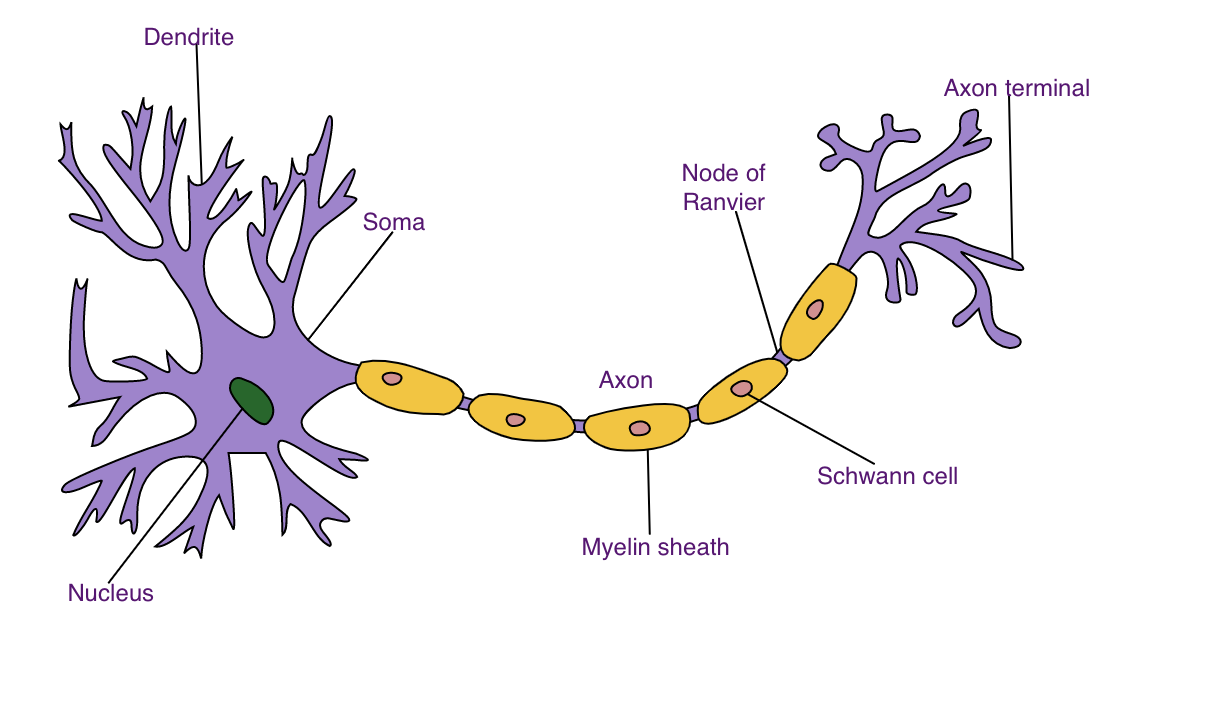
\includegraphics[width = \textwidth]{figures/Neuron.png}
  \caption{Overview about the main parts of a Neuron \cite{wikiNeuron}}
  \label{fig:neuronShema}
\end{figure}
The main part of a cell is called soma. It is the  body of a cell and holds the nucleus. Together they are responsible for keeping the cell alive as well as for reproduction, as the nucleus also holds the DNA.
The treelike structure reaching out from the Soma is called Dendrite. The different branches end near the axons of other cells and accept stimuli from them. It also tends to branch out from few main stems, channeling the connection from many other cells. Stimuli from other neurons change the electrical potential of the cell membrane. While the membrane potential degrades slowly over time, receiving enough excitation overcoming the decay, the potential rises to a threshold level and an electrical impulse discharges along the axon to the axon terminals resetting the membrane potential. The axon leads the signal to other neurons and largely varies in length as it may connect to other brain regions. In the area around the end of the axon it again branches out in small axon terminals connecting to the dendrit of different neurons. Human brains are estimated to have 86 billion neurons forming a complex network with their connection.
\newline
As the neurons are separate cells there is a gap between axon terminals and dendrit which is called Synaptic Gap. There are two main types of synapses differentiated by the way the information is passed. One type is based on electric transmission of the signal, the other uses chemicals to travel the gap and stimulate the neuron. The chemical transmission is believed to make up most of the connection and is also the one simulated by the spiking neural networks used for this thesis. In \autoref{fig:chemicalSynaps} the main parts building a chemical synapse are shown.
\begin{figure}[htpb]
  \centering
  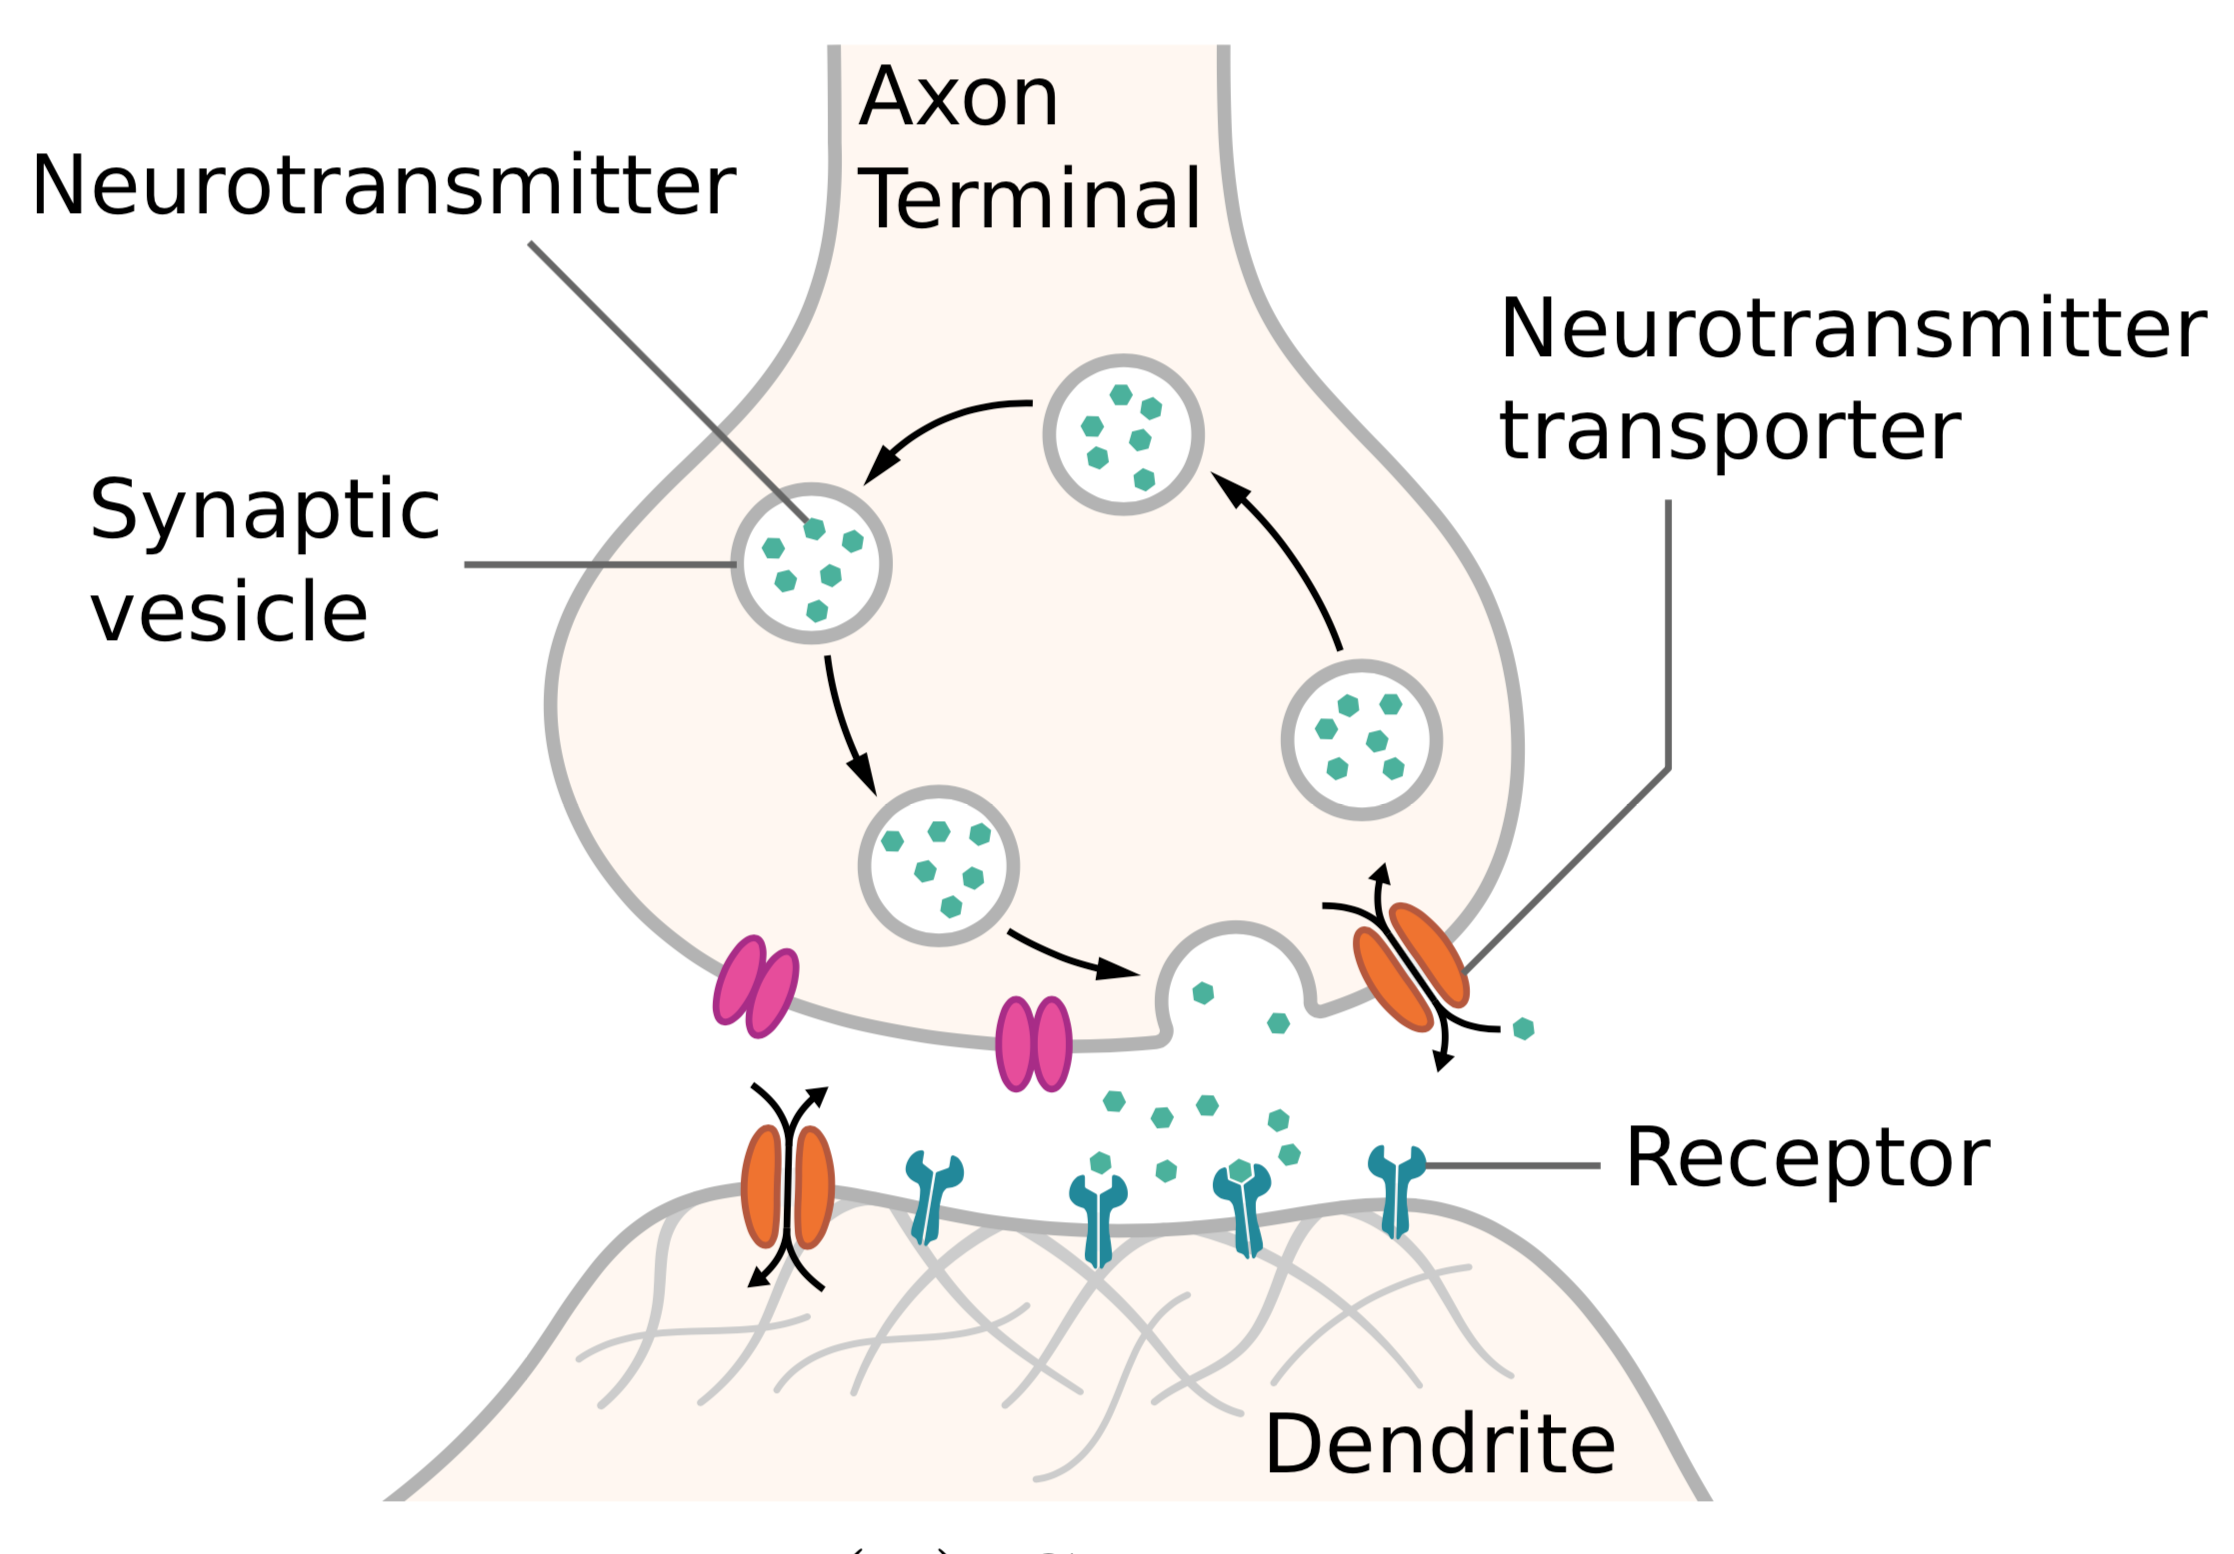
\includegraphics[scale=0.25]{figures/synapse.png}
  \caption{Schemata of a Synapse \cite{wikiSyn}}
  \label{fig:chemicalSynaps}
\end{figure}
To transmit an incoming signal the axon terminal releases neurotransmitters to the gap which can be received by the dendrit through receptors. Neurotransmitters are build in the terminal or reabsorbed from the gap. In the terminal they are held in Synaptic Vesicles which can fuse with voltage gated calcium channels releasing the transmitters to the gap\cite{Catterall411}. How good the connection transmits the signal depends mainly on the amount of neurotransmitters released as well as the amount of receptors at the dendrite. 
In the synaptic gap there also can be neuromodulators eg. Dopamine which are believed to change how the synapse evolves over time and thus amplify or diminish changes in the strength of the connection.

\section{Artificial Neural Networks}
To explore how these networks act the neurophysiologist Warren McCulloch and the mathematician Walter Pitts developed the first mathematical model in 1943 \cite{mcculloch1943logical}. This model, known as McCulloch-Pitts-Model is a strongly simplified description of a Neuron and shown in \autoref{fig:MCPShema}. It has binary inputs and a binary output. If the sum over the  inputs exceeds a threshold the output is $1$ otherwise it is $0$. Inventing the Perceptron Frank Rosenblatt proposed 1962 a model overcoming the limitations to boolean inputs and using real-valued weights on the inputs.
\begin{figure}[htpb]
  \centering
  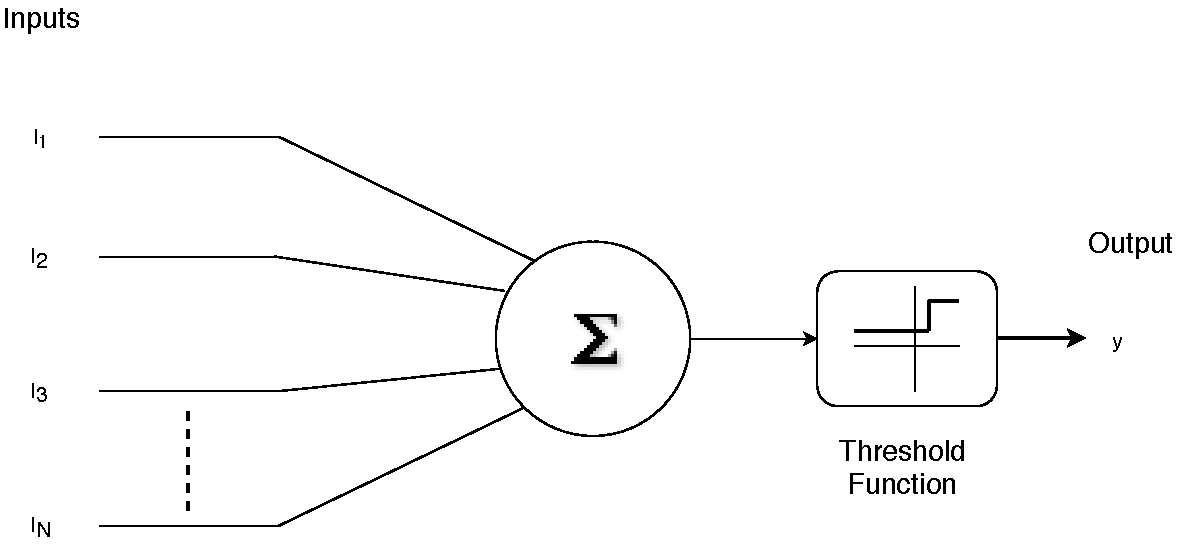
\includegraphics[scale=0.65]{figures/McPSchema.pdf}
  \caption[Schemata of McCulloch-Pitts-Model]{Schemata of a Synapse \cite{wikiSyn}}
  \label{fig:MCPShema}
\end{figure}
\newline
\autoref{eq:MCP} describes the behaviour of the perceptron where x is a real-valued input vector, w the vector of the weights of the same size and b a bias. 
\newline

\begin{equation}\label{eq:MCP}
  f(x) =
    \begin{cases}
      1 & \text{if $w*x+b > 0$,} \\
      0 & \text{otherwise.}
    \end{cases}  
\end{equation}
By choosing the right weights the perceptron can be used as classifier for linear separable data. Further it can be shown that weights can be learned and converge in linear separable training sets \cite{Bishop:998831}. The algorithm calculates the weight change from comparing the result $y_j$ calculated by the neuron from the feature set $x_j$, with the desired result $d_j$ for each training sample $j$. The weight change for every connection is the result of multiplying the error $d-y$ by the learning rate $r$ and the input $x$ of that connection as shown in \autoref{eq:MCP_weight} .
\newline
\begin{equation}\label{eq:MCP_weight}
  w_i(t+1) = w_i(t) +r * (d_j - y_j(t))*x_{ji} \text{ , for all features $0<=i<=n$}
\end{equation}
By iterating over the set of training samples and updating the weights after each step these converge to the correct values to classify the data.
\newline
For this learning rule the bias is described by setting $x_0$ always to $1$ and have the feature set of size n represented by $x_1$ to xn. Doing so $w_0$ acts as bias for the threshold function and gets adjusted in the learning process.

\section{Second generation of ANN}\label{sec:backprop}
To be able to solve non-linear classifiable data sets multiple perceptrons can be chained to form a network. This construct is referred as Multilayer Perceptron (MP) and consists of at least three layers, the input, hidden and output layer. Unlike a single perceptron the activation function of neurons in MPs are sigmoid shaped. Historically most common is the logistic function:
\begin{equation}\label{eq:logisFunc}
  y_i(v_i) = (1 + e^{-v_i})^{-1}
\end{equation}
where $y$ is the output of the $i$-th neuron for the weighted sum $v_i$ of its input connections.
\autoref{fig:logisFunction} shows the shape of this function.

\begin{figure}[htpb]
  \centering
  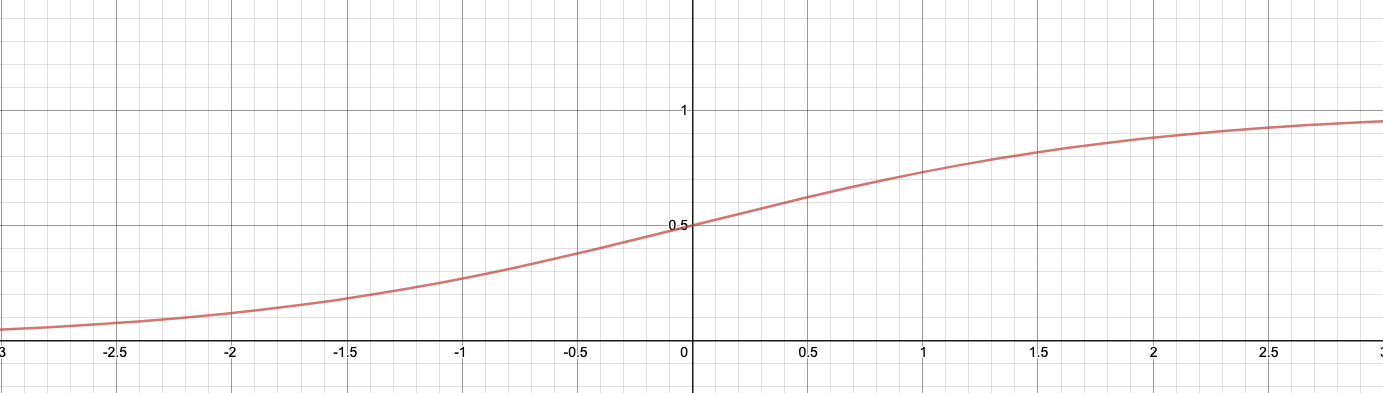
\includegraphics[width = \textwidth]{figures/logisticFunc.png}
  \caption{Plot of a logistic function}
  \label{fig:logisFunction}
\end{figure}
For learning the weights an algorithm called back-propagation was proposed 1986 by David Everett Rumelhart and others \cite{rumelhart1988learning}. It generalizes the learning function of the single perceptron. It consists of two main steps for each training sample. First the output for the feature set $x$ is calculated, which is also referenced as information forward propagation. The overall error is the sum of the squared difference in output $o$ to the target $t$ in each output node and is described by the following functions:
\begin{equation}\label{eq:backpErr}
  E = \frac{1}{2} \sum_{i=1}^n (t_i-o_i)^2
\end{equation}
The aim of the back-propagation algorithm is to minimize this error. This is realized by propagating the error in each output back through the network and changing the weights of each connection which is the second step and referred as error back propagation. In this step for each connection the partial derivative of the error with respect to its weight is calculated which describes the impact a change of this weight has on the error and in which direction it changes the error. For each connection this depends on the impact it has on the result oj of the node it connects to and its impact on the error.
\newline
This can formally be described by the first step in this equation:
\begin{equation}\label{eq:backpMainDevi}
  \frac{\partial E}{\partial w_{ij}} =
  \frac{\partial E}{\partial o_j} \frac{\partial o_j}{\partial w_{ij}} = 
  \frac{\partial E}{\partial o_j} \frac{\partial o_j}{\partial net_j} \frac{\partial net_j}{\partial w_{ij}}
\end{equation}

The impact on the output in $o_j$ is dependent on the weights influence on the activation sum $net_j$ of a node, what is used in the second step. In this last factor only one term in the sum depends on $w_{ij}$ thus its derivat is $o_i$
\begin{equation}\label{eq:backp3s}
  \frac{\partial net_j}{\partial w_{ij}} =  \frac{\partial}{\partial w_{ij}} \left( \sum_{k=1}^n w_{kj} o_{kj} \right) = \frac{\partial}{\partial w_{ij}} w_{ij}o_i = o_i
\end{equation}
The second factor in \autoref{eq:backpMainDevi} is the derivative of the output of a node with respect to its input which is the partial derivative of the used activation function and also the reason backpropagation needs a differentiable activation function.
\newline
For connections to output neurons $o_j$ equals to $y_i$ and the first factor can be rewritten as
\begin{equation}
  \frac{\partial E}{\partial o_j} = \frac{\partial E}{\partial y_j} 
\end{equation}
The derivative for the square error from \autoref{eq:backpErr} again only depending in one sum on $y$ resolves to
\begin{equation}\label{eq:backpResEDev}
  \frac{\partial E}{\partial o_j} = \frac{\partial E}{\partial y_j} =
  \frac{\partial}{\partial y_j} \frac{1}{2}(t-y)^2 = y - t 
\end{equation}
Plugging everything together through substitution, the derivative can be rewritten as 
\begin{equation}
  \frac{\partial E}{\partial w_{ij}} = o_i \delta_j
\end{equation}
with
\begin{equation}
  \delta_j = \frac{\partial E}{\partial o_j}\frac{\partial o_j}{\partial net_j} =
  \begin{cases}
    \frac{\partial L(o_j,t)}{\partial o_j}\frac{\partial \varphi (net_j)}{\partial net_j} & \text{if $j$ is an output neuron,}\\
    (\sum_{l \in L} w_{jl}\delta_l ) \frac{\partial \varphi(net_j)}{\partial net_j} & \text{if j is an inner neuron.}
  \end{cases}
\end{equation}
Where $L$ represents the loss function which in our case is $(t-y)^2$ and $\varphi$ the activation function in \autoref{eq:logisFunc}. For these the derivatives simplify to
\begin{equation}
  \delta_j = \frac{\partial E}{\partial o_j}\frac{\partial o_j}{\partial net_j} =
  \begin{cases}
    (o_j - t_j) o_j (1-o_j) & \text{if $j$ is an output neuron,}\\
    (\sum_{l \in L} w_{jl}\delta_l ) o_j (1-o_j) & \text{if j is an inner neuron.}
  \end{cases}
\end{equation}
The weight change of the connection from node $i$ to node $j$ is calculated by following equation
\begin{equation}
  \Delta w_{ij} = -\eta \frac{\partial E}{\partial w_{ij}} = - \eta o_i \delta_j
\end{equation}
where the gradient is multiplied by $n_y > 0$ which is the learning rate and can be thought as small step along the gradient. Is the gradient positive an increase in $w_{ij}$ would increase $E$ and vice versa. Therefore the negative gradient is used as the minimum for the function should be found. As for inner notes its $\delta$ is recursively defined by the $\delta$ of all nodes it connects to, the weight change depends on the error information traveling from the output layer backwards to the input layer\cite{sporea2013supervised}.
\newline
While the model of a neuron in the MP is not simulating electrical pulses as they occur in biological neurons the activation level of the artificial ones can be viewed as an abstraction of the mean spike rate of that neuron.



\section{Spiking Neural Networks}

The neuron model used in Spiking Neural Networks closes the gap to real neurons even further by communicating through impulses. Unlike the previous generations, neurons can activate and send out an impulse at any time rather than have an activation level at discrete timesteps. This adds spatial-temporal information to the dynamics of the network and in theory it has been shown that these networks are more powerful than their predecessors and considered the third generation of artificial neural networks \cite{maass1997networks}.
\newline
The change to spike events as encoding information brings several changes to the mathematical description of the neurons and synapses.

\subsection{Leaky Integrate-and-Fire Neuron}
Probably the best known model used for neurons in this regard is the Leaky Integrate and Fire model. In this model the membrane is thought of as electric capacitor which losses potential over time. The derivative of the membrane Voltage $V$ is calculated by the function
\begin{equation}
  \frac{\partial V}{\partial t} = - \frac{1}{\tau_m}V + \frac{1}{C_m}I(t)
\end{equation}

$\tau_m$ is the membrane time constant inversely scaling the loss of voltage,  $I(t)$ is the sum of all incoming current at time $t$ and $c_m$ is the capacity of the membrane. This holds in case of the potential being smaller than the threshold value. As soon as the threshold is reached the neuron fires and for the refractory period $tau_{ref}$ its potential is set to the reset potential $V_{reset}$. The current $I_{syn}$ of the spike released to another neuron is determined by the function
\begin{equation}
  I_{syn}(t)=we^{\frac{-t}{\tau_{syn}}}
\end{equation}

with $w$ being the weight of the synapse connecting the neurons and $t_{syn}$ being the synaptic time constant.

\subsection{Stdp learning}
The Hebbian rule was proposed by psychologist Donald Hebb in 1949 claiming that the connection from neuron \textbf{A} to neuron \textbf{B} should be strengthened if \textbf{A} consistently takes part in firing \textbf{B}. Which is often simplified to “Cells that fire together, wire together”. As the learning happens without influences it can be categorized as unsupervised learning.
One shortcoming of the Hebbian rule is that it doesn’t cover depression of a connection as well as that to take part in the firing of a neuron the presynaptic neuron has to fire not at the same time but slightly before the postsynaptic neuron.
Later experiments by Henry Markram suggested that the plasticity of a synapse is changed by exact timings of spikes in the pre- and postsynaptic membranes. If the presynaptic spike is followed by a postsynaptic one the connection is strengthened in the other case weakened.
The time difference $delta_t$ is
\begin{equation}
  \Delta t = t_{post} - t_{pre}
\end{equation}
and is used for calculating the weight change defined by
\begin{equation}
  STDP(\Delta t) = 
  \begin{cases}
    A_+ e^{-\frac{\vert \Delta t \vert }{\tau_+}} & \text{if $\Delta t>0$} \\
    A_- e^{-\frac{\vert \Delta t \vert }{\tau_-}} & \text{if $\Delta t<=0$} \\
  \end{cases}
\end{equation}
with $A_+$ and $A_-$ as scaling factors for potentiation and depression and $\tau_-$ and $\tau_+$ defining the height of the learning window. \autoref{fig:STDP}

\begin{figure}[htpb]
  \centering
  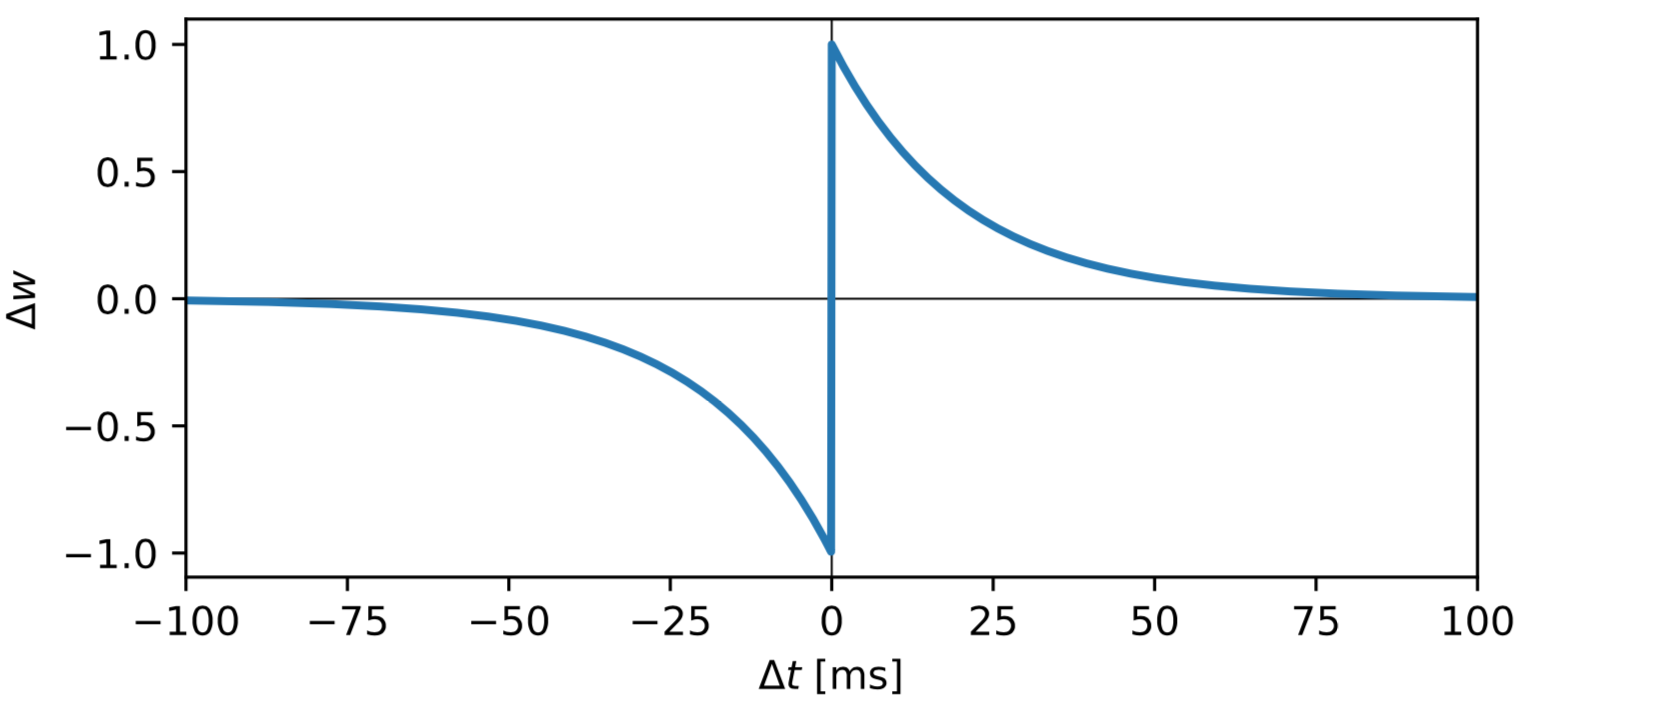
\includegraphics[width = \textwidth]{figures/STDPcurve.png}
  \caption{Plot of the STDP learning window}
  \label{fig:STDP}
\end{figure}

shows the plot of the STDP learning function for $A_+$ and $A_-$ of the same magnitude of $1$, setting the maximum values for the function.

\subsection{R-STDP}
In 2007 Izhikevich proposed a learning rule for Reward-modulated Spike-Timing-Dependent-Pasticity.  In his model the weight changes calculated by the STDP mechanism are collected in an eligibility trace rather then be applied directly. This is necessary as the reward from the environment is not available at the time of the spike event and can thus not be factored in for modifying the weight. The change of the eligibility trace is defined by
\begin{equation}
  \dot{c} = - \frac{c}{\tau_c} + STDP(\Delta t) \delta(t-s_{pre/post})C_1 \text{ ,}
\end{equation}
where $\tau_c$ is the time constant, $\delta$ thet dirac delta function, $s_{pre/post}$ the timing of the second spike of a spike pair $s_{pre}$ and $s_{post}$ and $C_1$ a constant coefficient. If no spikes occur the eligibility will decay. Only at the time of the second spike the result of the STDP learning rule multiplied by the coefficient is added, which will increase the eligibility if the presynaptic spike occurs before the postsynaptic. The dynamics of the reward are described by
\begin{equation}
  \dot{n}=-\frac{n}{\tau_n} + \frac{\delta(t-s_n)}{\tau_n}C_2 \text{ ,}
\end{equation}

here $n$ is the neuromodulator concentration, $\tau_n$ its time constant, $s_n$ the spike time of the neuromodulator and $C_2$ a constant coefficient.
The weight change according to R-STDP is then given by
\begin{equation} \label{eq:dWrStdp}
\dot{w}=c(n-b)
\end{equation}

With $b$ being the baseline concentration of the neuromodulator. A visualisation of this dynamic is shown in \autoref{fig:RSTDPlearn} taken from and further described in \cite{legenstein2008learning}.  \textbf{A} shows the eligibility function for a positive STDP outcome with the second spike time at $t = 0$. The second part \textbf{B} shows in the first row the spike-trains of the connected neurons. In the second row the red line is the effect of a positive STDP result on the eligibility trace, green the effect of a negative one and black the resulting eligibility. The third row displays the neuromodulator concentration with a spike occurring and the fourth row displays how the weight changes in this scenario.


\begin{figure}[htpb]
  \centering
  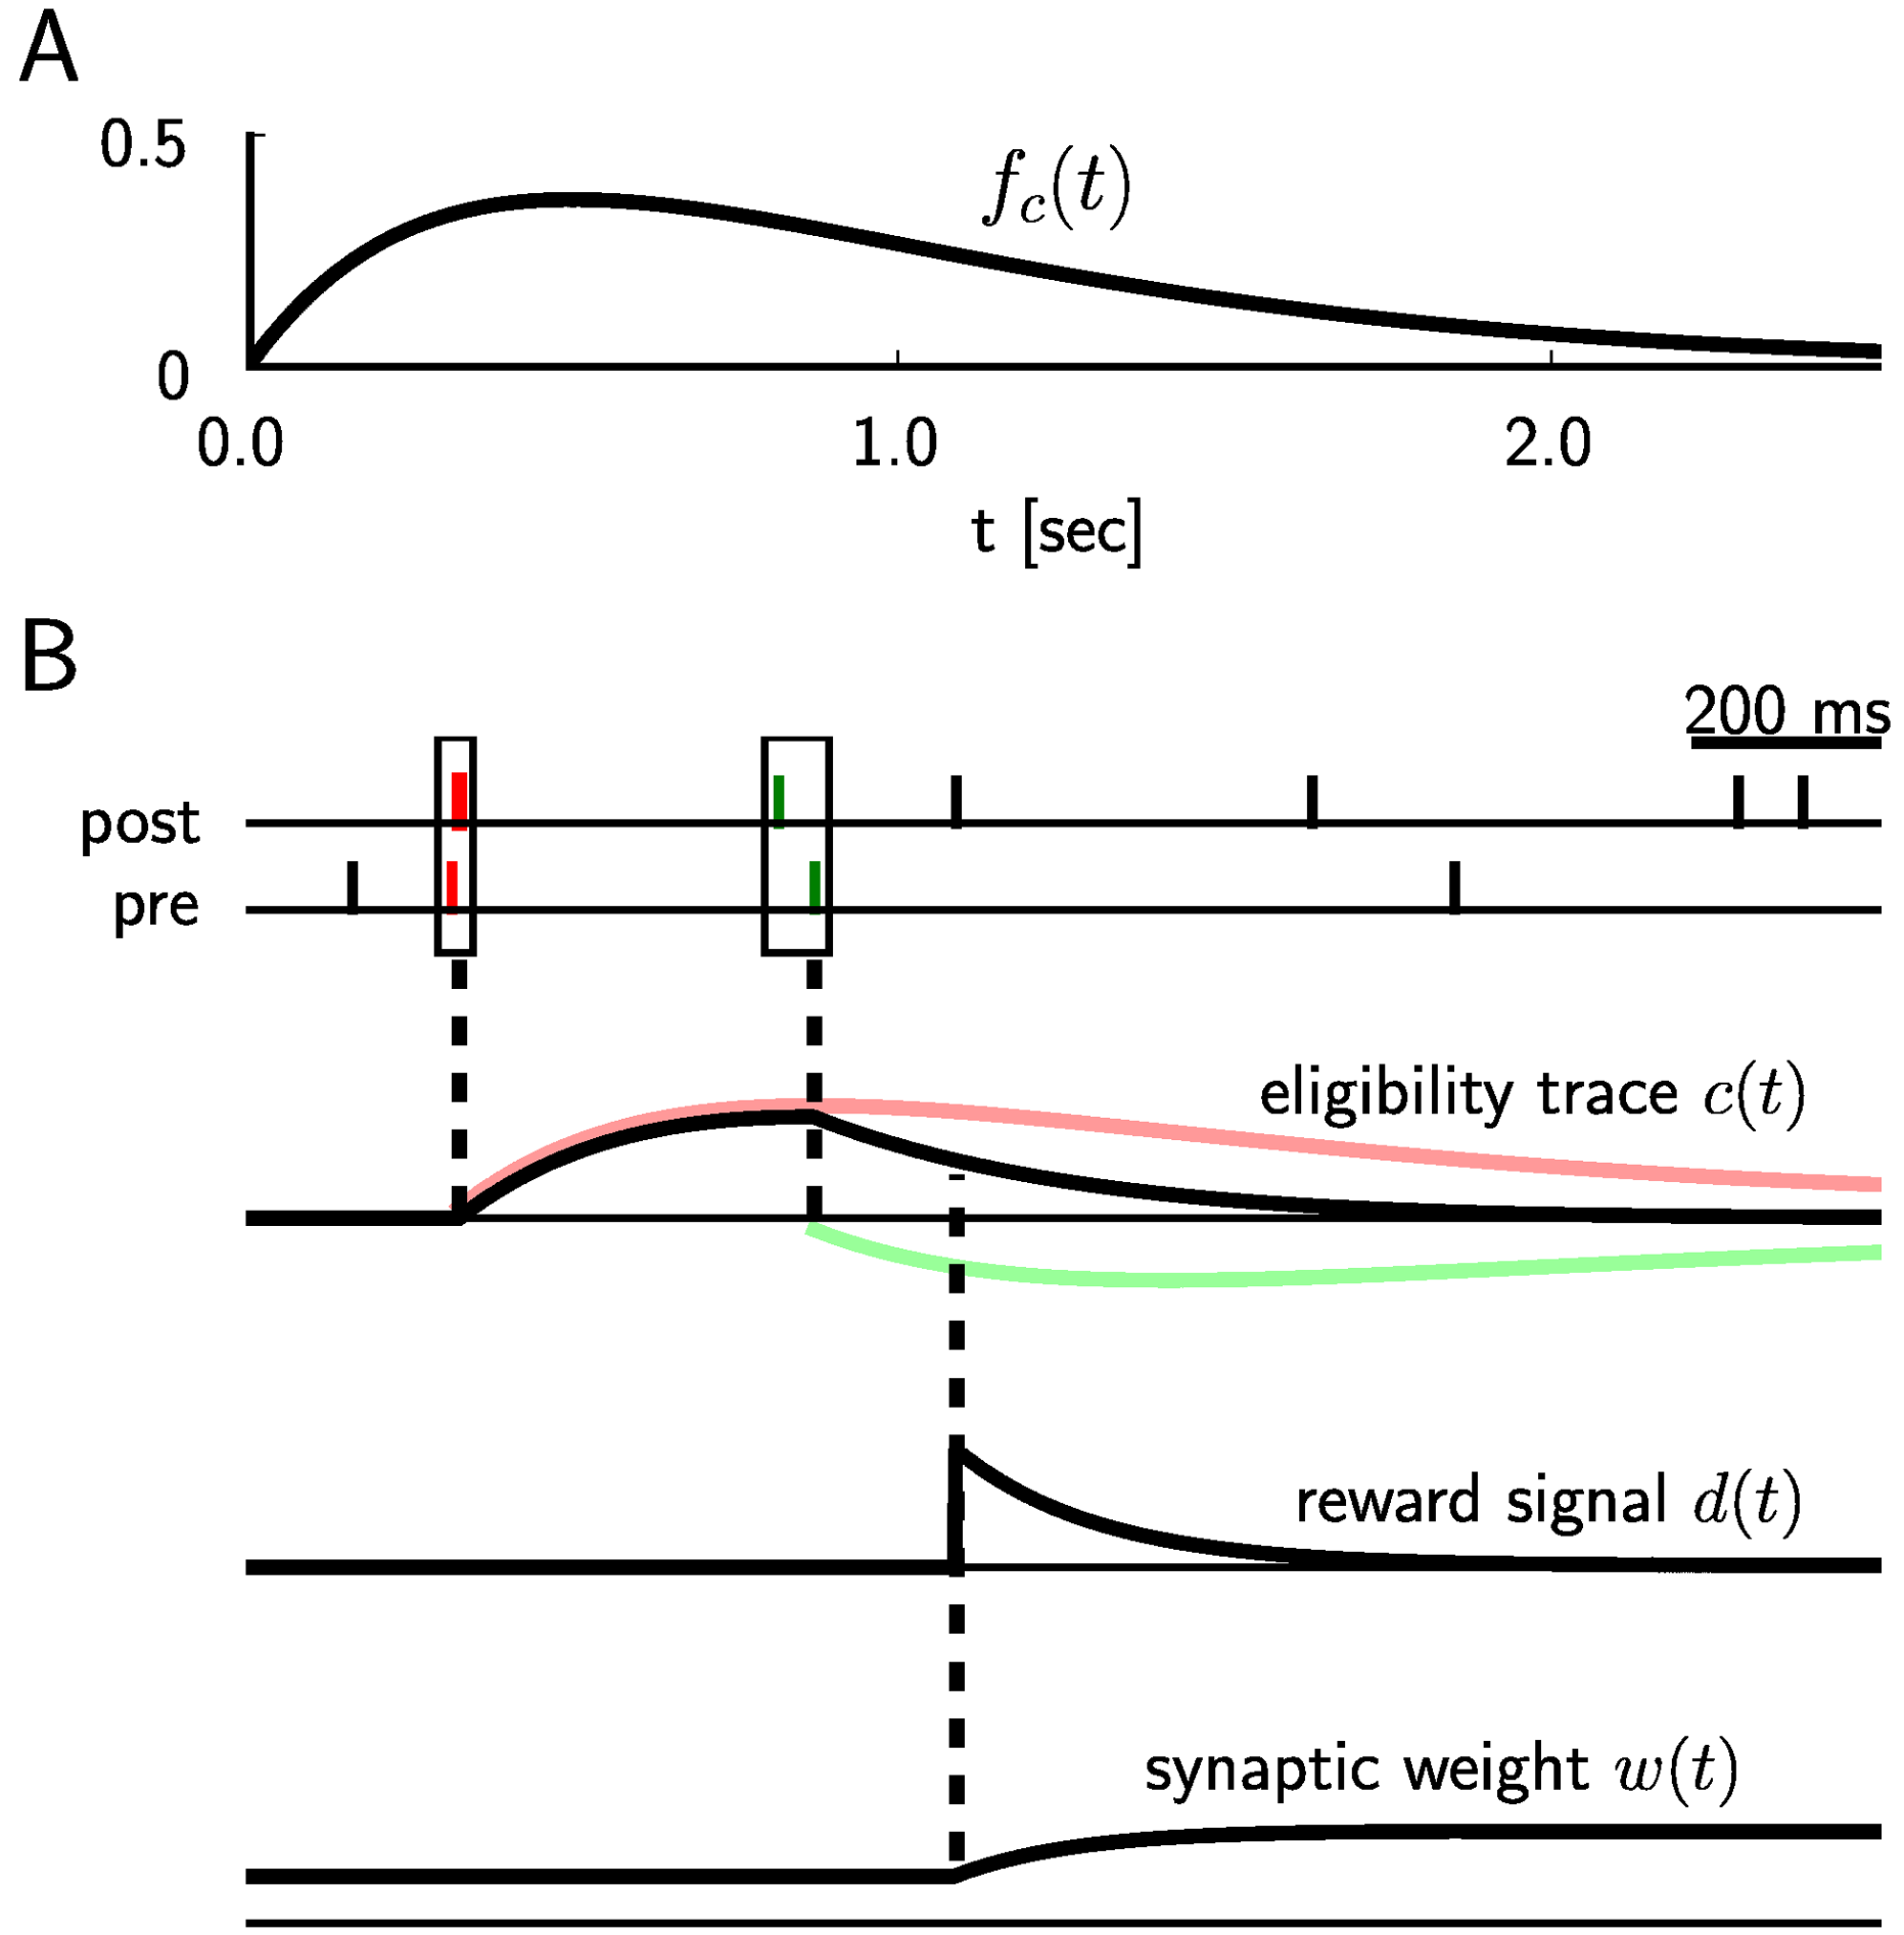
\includegraphics[scale=3]{figures/rstdp.png}
  \caption[R-STDP meachanic]{In his paper Legenstein described the R-Stdp Mechanism
  \cite{legenstein2008learning}:\newline
  (A) Eligibility function $f_c(t)$, which scales the contribution of a pre/post spike pair (with the second spike at time 0) to the eligibility trace $c(t)$ at time $t$. (B) Contribution of a pre-before-post spike pair (in red) and a post-before-pre spike pair (in green) to the eligibility trace $c(t)$ (in black), which is the sum of the red and green curves.}
  \label{fig:RSTDPlearn}
\end{figure}
% \begin{figure}[t]
%   \includegraphics[width=\textwidth]{activity-diagrams/Assessment_Workflow_Old_Simple}
%   \caption{UML activity diagram of the semi-automatic assessment workflow in the current system based on Otter \cite{otter2018thesis}. Every modeling submission is either assessed automatically by \textit{Compass} or manually by a tutor.}
%   \label{fig:assessment_workflow_old_simple}
% \end{figure}

In the experiments described in this thesis the Leaky Integrate-and-Fire Neuron will be used in combination of the R-STDP learning rule for synaptic weights to build spiking neural networks.

\subsection{Dynamic Vision Sensor}
While conventional cameras are getting better and better this is not particularly great for robotic and autonomous mobile applications. The reason is that newer cameras tend to have a higher resolution or refresh rate of their frames causing a higher data volume from the cameras. The data probably includes more information then cameras delivered a year ago but more data also means more work to do not only analysing it but also just by handling it. This leads to the consumption of more energy and waiting for processing to happen can be a hindrance for real time applications. Thus for robotic vision an optical system is needed, that reduces data load while keeping up the information flow from the real world to the system. The huge amount of data of cameras is structured in frames and the frames contain the information of their pixels. This way of capturing video data is called framebased. 
Especially for tasks with fast moving objects a very high frame rate is needed. This leads to a huge amount of overhead as most pixels in each frame tend to have almost the same values in the next frame and thus the data for these pixels has no additional information. New information is only introduced if the value of a pixel changes meaningfully.
\newline
To only transmit data if there is a meaningful change is the concept behind Dynamic Vision Sensors DVS entering the market only in recent years. Their functional principles are often compared to the one of the human retina as their receptor circuits keep track of the change in luminance and are able to send events at any time the change overcomes a threshold. The events are sent from the camera over an eventbus and can be described as the tuple $<x,y,t,p>$ containing the $x$ and $y$ coordinates of the pixel, the time the event occurred and the polarity of the change. This event based principle enables the camera to achieve a very high time resolution, at the moment in the area of microseconds. Furthermore, the similarity between the events of a DVS camera to spikes makes these sensors ideal for the use with SNNs.
For a better understanding it is helpful to keep in mind that in no point in time a complete picture of the environment is present in the system and thus the output for a completely static environment would be entirely black. For a rotating dot the graphic in \autoref{fig:rotatingDot} shows the output of a dvs sensor over time as well as a slice, accumulating the events over 300 microseconds. The graphics is the result of experiments done by Lichtensteiner and are more closely described in his paper \cite{lichtsteiner2008128}.

\begin{figure}[htpb]
  \centering
  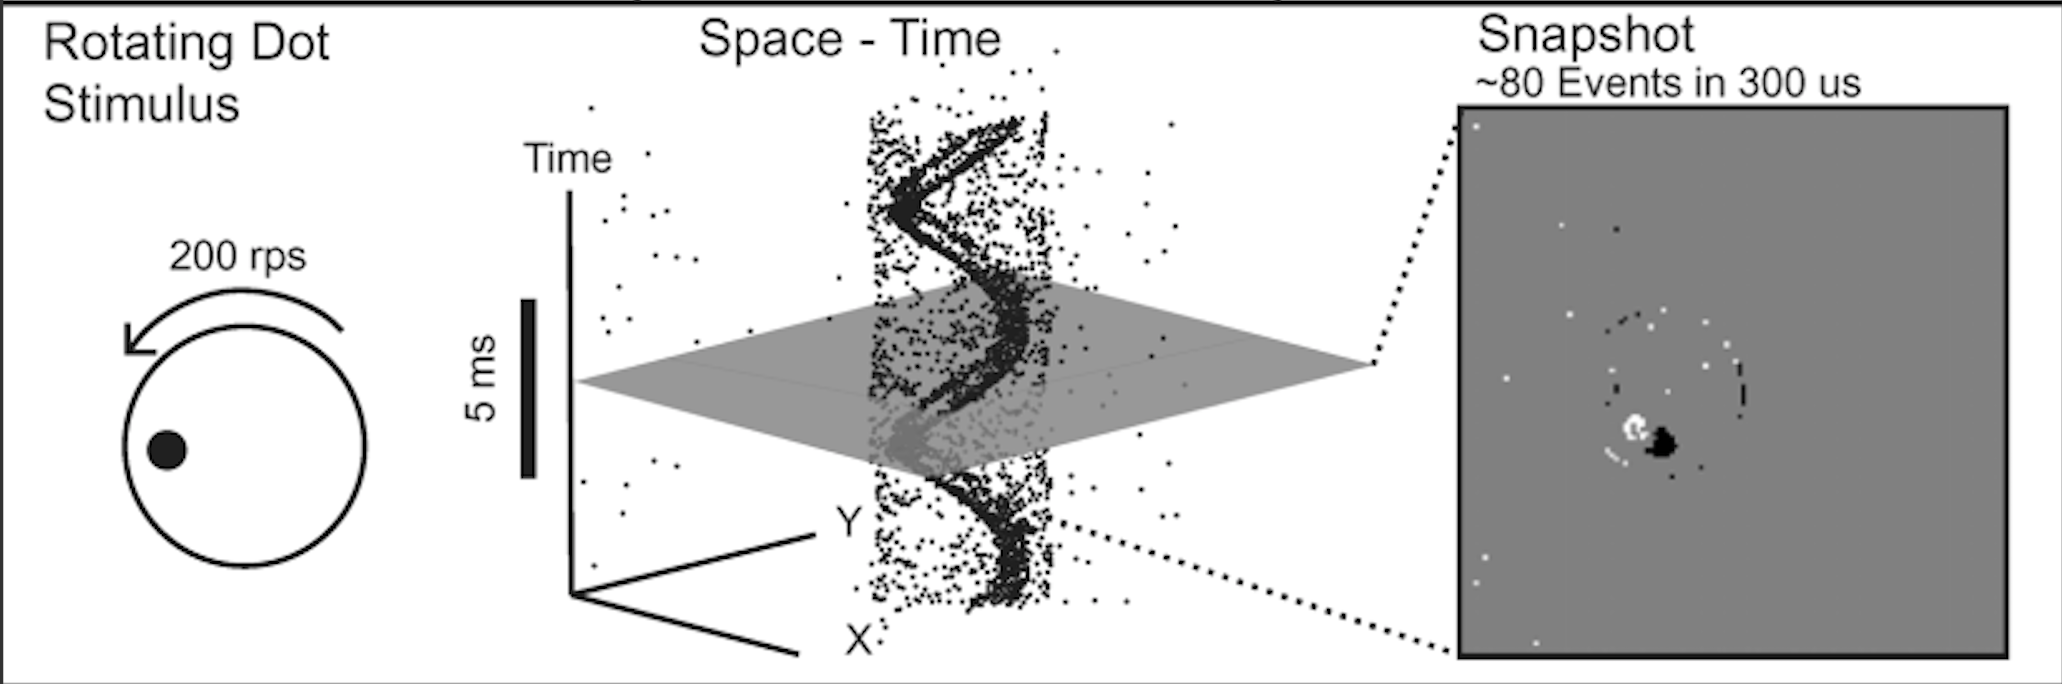
\includegraphics[width=\textwidth]{figures/rotatingDot}
  \newline
  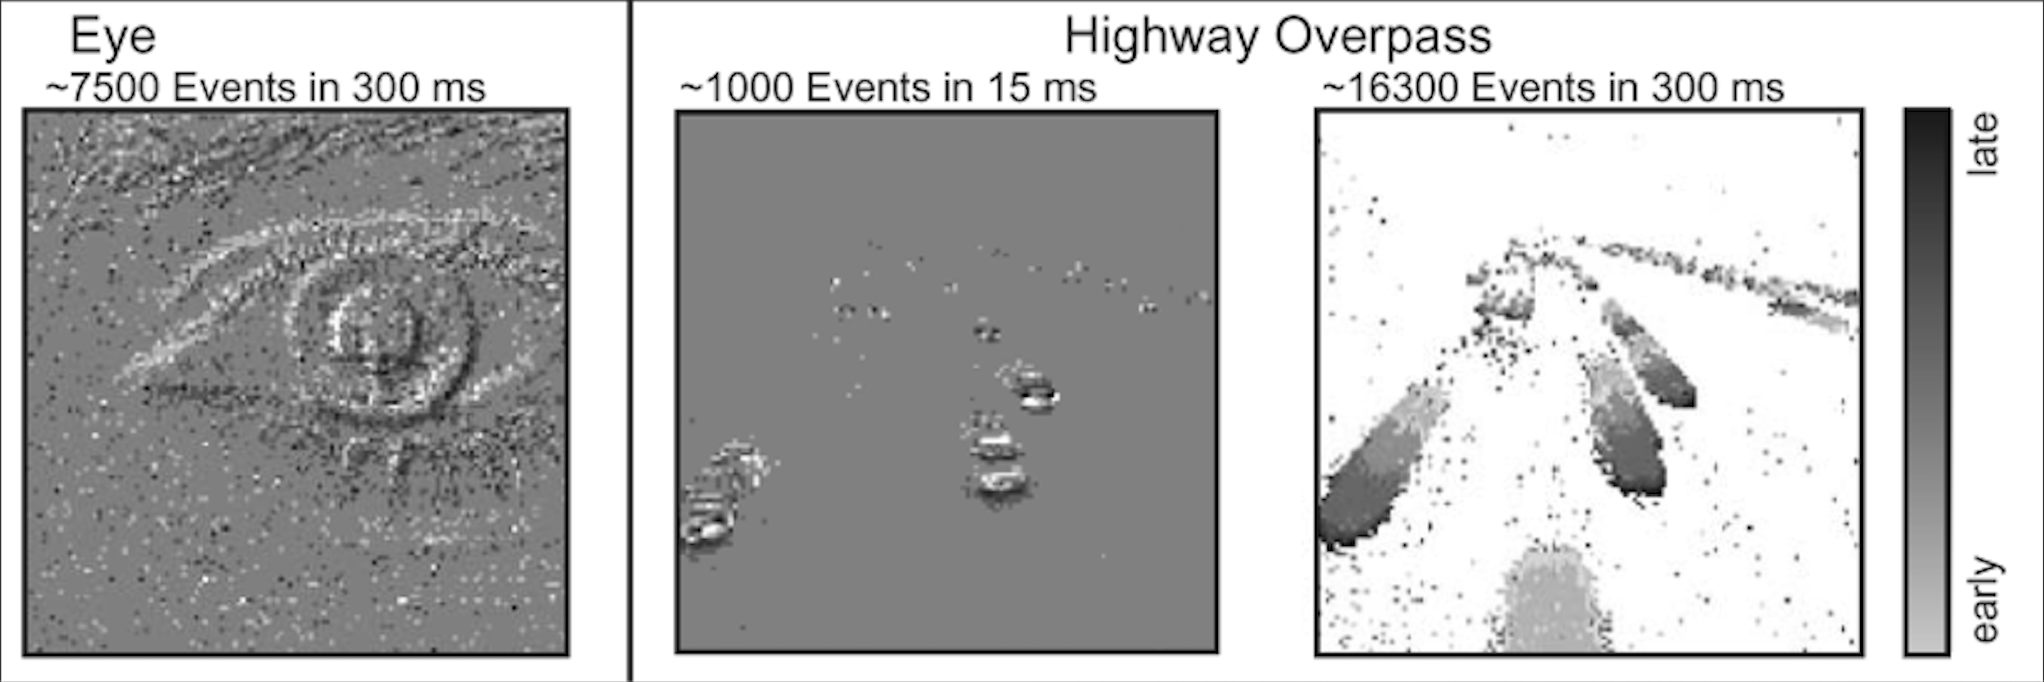
\includegraphics[width=\textwidth]{figures/rotatingDotAdd}
  \caption{Rotating Dot stimulus visualised over time and additional Dvs pictures}
  \label{fig:rotatingDot}
\end{figure}
The other examples are different scenes where either the camera was moved, resulting in the darker images, or the camera was static resulting in the bright images where white means that no event was detected for that pixel over the time period of accumulation.


\subsection{Snake like Robot}
The Robot used for the experiments tries to reassemble the shape and degrees of freedom a snake has. Unlike to a real snake, which can continuously curve its body, the robot has a modular design with rotational joints between the modules. The axes of the joints are rotated by 90º along the body axe enabling three dimensional movement with abundant degrees of freedom. This allows the robot to perform snake like movement patterns like slithering, climbing and sidewinding as well as rolling sidewards in an arch shaped body configuration, but various other movement patterns can also be thought of depending on environment. Examples for these different gaits are shown in \autoref{fig:snakeGaits} made by Jiang for a presentation\cite{snakeRobo}.
\newline
\begin{figure}[htpb]
  \centering
  \includegraphics[width=\textwidth]{figures/roboGates.png}
  \caption{Slide of Presentation by Jiang showing the different gaits of the robot\cite{snakeRobo}}
  \label{fig:snakeGaits}
\end{figure}
Snake like robots can navigate through tiny space like pipes and holes as well are also able to climb. That makes them especially interesting for the use in difficult terrain such as in rescue missions after earthquakes.
For the experiments the slithering gait is used and the network only tells the robot in which direction it should go. In the slithering gait the robots head will move from one side to the other while keeping its orientation parallel to the movement direction. In this way it is able to sense the environment in front while moving. As a result of this movement pattern objects in front of the robot will change their position in sensing area throughout the motion.

\subsection{Neuro Robotics Platform}
The experiments done in this paper where simulated in the Neuro Robotics Platform (NRP) \cite{nrp} developed in the Human Brain Project \cite{hbp}. NRP enables the physical simulation of robots in environments as well as the integration of SNN to control the robots and thus gives the boilerplate to conduct experiments. Its core is a Closed Loop Engine (CLE) synchronizing the simulation of the SNN in NEST and the simulation of the world in ROS/Gazebo. To do so it pauses both simulations after a defined timespan and exchanges data between the simulations and updating their state. The interaction between the environment and the SNN is defined in Transfer Functions (TF) which for example set the target angles for each joint of the snake.




% \begin{figure}[t]
%   \includegraphics[width=\textwidth]{activity-diagrams/Assessment_Workflow_Old_Simple}
%   \caption{UML activity diagram of the semi-automatic assessment workflow in the current system based on Otter \cite{otter2018thesis}. Every modeling submission is either assessed automatically by \textit{Compass} or manually by a tutor.}
%   \label{fig:assessment_workflow_old_simple}
% \end{figure}


% !TeX root = ../main.tex
% Add the above to each chapter to make compiling the PDF easier in some editors.

\chapter{Methodology}\label{chapter:Methology}
In this section the setup for the simulation as well as the transfer functions used for the data exchange are described.

\section{Simulation Environment}
In the simulation the robot is placed in an empty environment with only a ball as target in front of it. The ball has a radius of $30$ centimeters and is placed $1.6$ meters in front of the robot. A screenshot of the configuration in starting position is shown in \autoref{fig:startingPosRobo}. During the simulation the target moves along a predefined path and the snake is supposed to follow it. When the angle between the orientation of the snake head and the target surpass a certain threshold the simulation is paused, the snake and the target are reset to their starting positions and the simulation is unpaused. The path of the target is mirrored after each reset. As step size for the CLE a time span of $20$ milliseconds is used.

\begin{figure}[htpb]
  \centering
  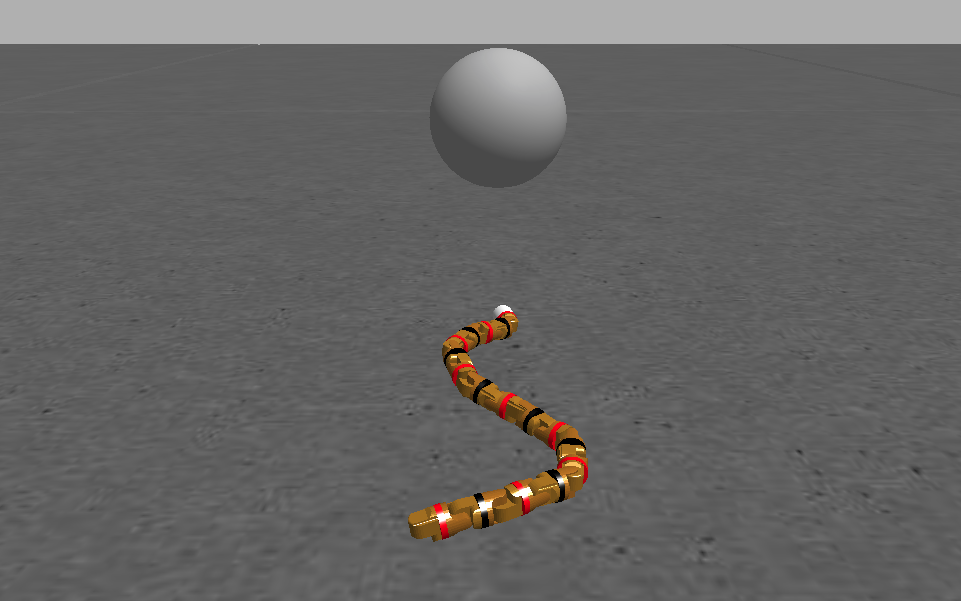
\includegraphics[width=\textwidth]{figures/startingPosition.png}
  \caption{View of the simulation in the starting/reset configuration }
  \label{fig:startingPosRobo}
\end{figure}



\section{Transmitting DVS}
Simulating real DVS data is difficult as the time resolution of DVSs is much higher than the simulation step size. For the experiments a Gazebo plugin developed by Kaiser and Colleagues was used simulating a DVS data stream\cite{kaiser2016towards}. The plugin uses the information provided by a virtual camera mounted in the snakes head to calculate the difference in brightness for each pixel compared to the buffered value of the last timestep. For each pixel exceeding the threshold of $10$ percent a DVS event is created. 
As result events generated in the simulation all happen at the same time.
In their paper \cite{kaiser2016towards} Kaiser and Colleagues compare the output of the simulated output stream with a real one which is shown in \autoref{fig:realDVS}. It is clearly visible that the simulated output has events only in discrete time intervals and has much less noise then the real data.

\begin{figure}[htpb]
  \centering
  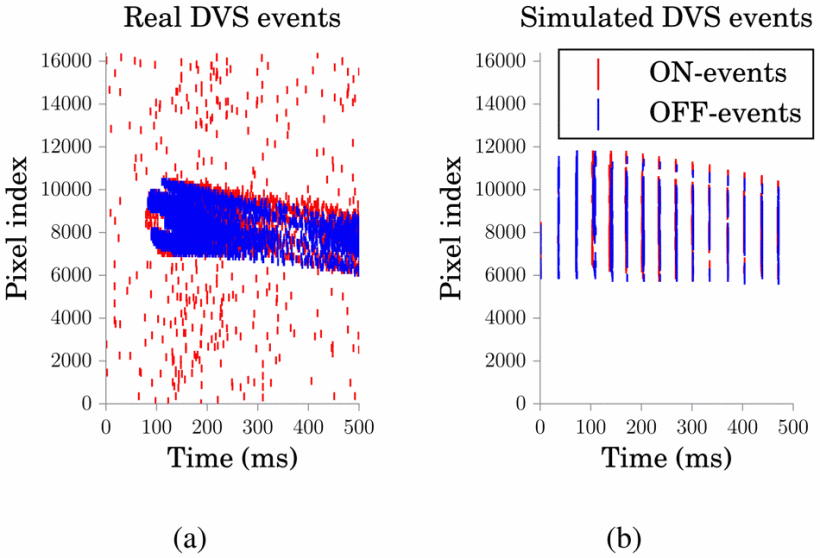
\includegraphics[width=\textwidth]{figures/realDvs.png}
  \caption{Comparison of DVS events generated by a real device (a) and by the simulation (b) \cite{kaiser2016towards}}
  \label{fig:realDVS}
\end{figure}
The simulated sensor has a resolution of $128$ by $128$ pixels. To reduce the complexity of the simulation for the SNN we are not using one input neuron for each pixel but group pixels up to superpixels. Additionally we crob of the bottom $50$ pixel rows as well as the top $20$ pixel rows, as those don't contain as much relevant data as the rest. \autoref{fig:dvsView} shows a rendering of the DVS output at a single simulation timestep and the outlines of the superpixels where in this case two rows of five pixels each were used.

\begin{figure}[htpb]
  \centering
  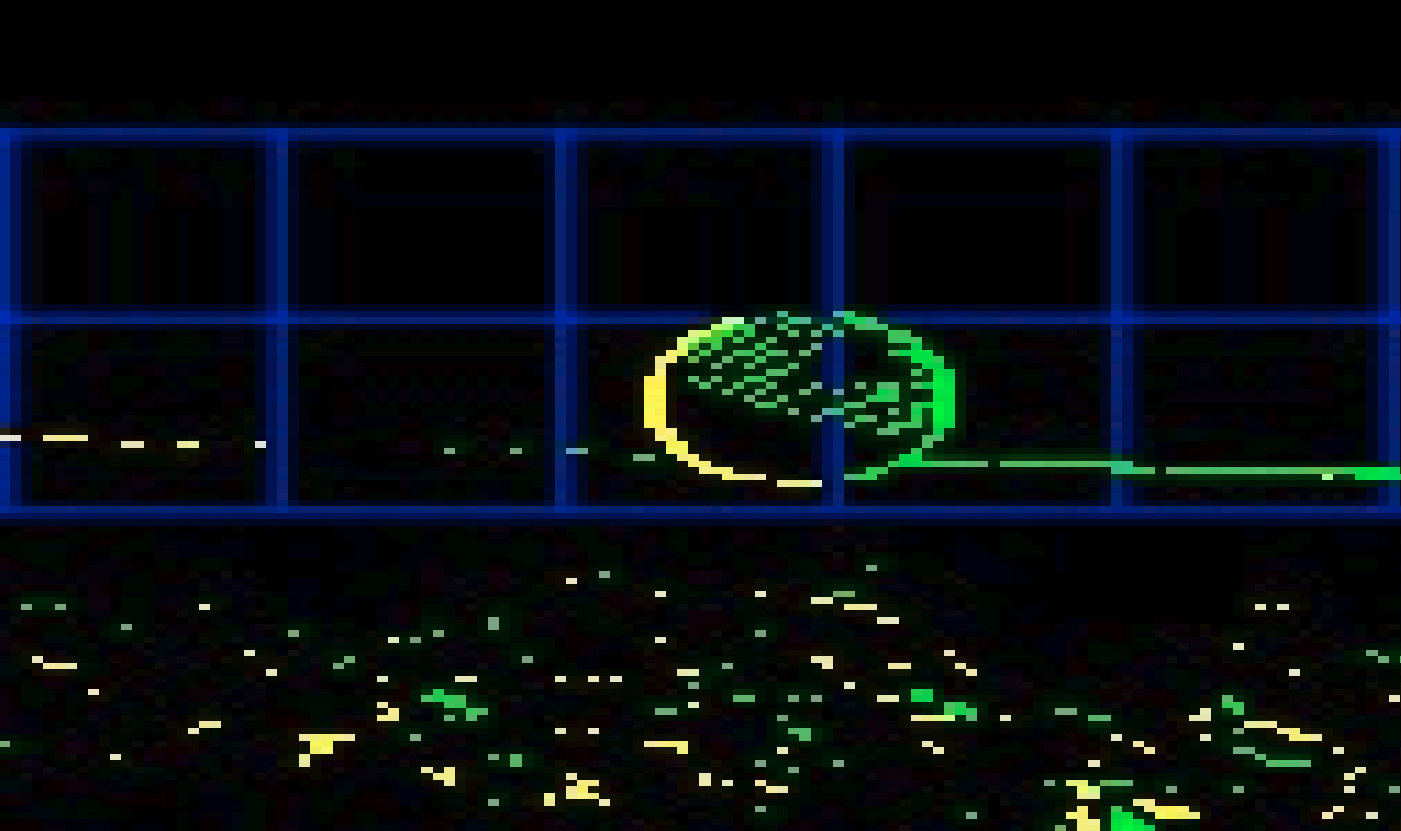
\includegraphics[width=\textwidth]{figures/DvsView.png}
  \caption{Snapshot of the output from the simulated DVS device. The blue lines show the boarder of the superpixels}
  \label{fig:dvsView}
\end{figure}

As the events occur all at the same time but represent the accumulated change over the past timestep, the events are spread out over one timestep. This is done by sending spikes to the network at a certain frequency, proportional to the number of spikes, $N_{events}$, the superpixel received. The frequency $f$ is then calculated by the following function:
\begin{equation}
  f = N_{events} * 50
\end{equation}
The factor at the end results from the simulation timestep lasting one fiftieth of a second thus the frequency $f$, measured in $Hz$, must be $50$ times that high.  Each superpixel has a corresponding Poisson neuron as input for the neural network, which is set to spike at the calculated frequency for the next timestep.
\newline
The input neurons are represented as array with its IDs counting the superpixel from left to right and bottom to top.

\section{Encoding of Joint Angles}\label{sec:EnOfJoint}
For some experiments the angle of some joints of the robot are used as an additional input for the neural network. Each joint angle is represented by two poisson neurons, one spiking proportional to the positive angle, one proportional to the negative angle. The angle $\beta$ is measured from the orientational axe of the module the joint is mounted on (module 1), which is shown in \autoref{fig:robAngle}

\begin{figure}[htpb]
  \centering
  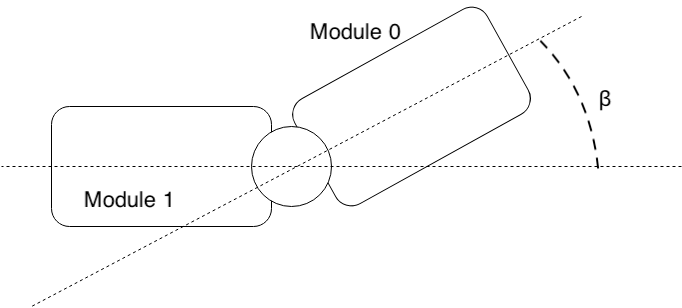
\includegraphics[width=\textwidth]{figures/roboAngle.png}
  \caption[Sketch of joint angle]{This sketch shows how the angle for a joint is measured. The angle $\beta$ of the joint between the two modules would be in this case around $-30$ degree}
  \label{fig:robAngle}
\end{figure}


With this setup only one neuron is active at a time and it’s spike frequency is given by the following equation:
\begin{equation}
  f_R = max(0., a * c)
\end{equation}
for the neuron signaling a positive angle and 
\begin{equation}
  f_L = max(0., - a * c)
\end{equation}
for the neuron signaling a negative angle. In the functions $a$ is the angle of the joint in degree and $c$ is a constant coefficient. This can be interpreted as the activity of neurons controlling the antagonist or respectively the agonist of a joint.

\section{Output Decoding}\label{sec:OutputDecoding}
The output for the used network is as well represented by two neurons, one for signaling the intention to go right, one for going left. To access the total number of spikes occurred on the outputs, each is connected to a spike recorder which keeps track of the spike history.
After each simulation step the number of spikes at the output is retrieved from its spike recorder and the spike recorder gets reset. From the difference in spike events the general direction is derived. This is then scaled by the mean number of spike events occurred on the nodes,which is shown in the following functions:
\begin{equation}
  N_d = N_r - N_l \\
\end{equation}
\begin{equation}
  D = N_d / (0.5 * (N_r + N_l)) \text{, with $D=[-2;2]$} 
\end{equation}
\begin{equation}
  D_{norm} = 0.5 * D = N_d/(N_r+N_l) 
\end{equation}
where $N_r$ and $N_l$ are the total number of spikes for the right/left neuron, $D_{norm}$ can be seen as the direction scaled by certainty, as its absolute value gets bigger the more exclusive the spikes occur on one neuron. By this interpretation of $D_{norm}$ representing the intention of changing the current direction $D_{t-1}$, the resulting direction $D_t$ is calculated by 
\label{eg:OutputCalc}
\begin{equation}
  D_t = min(1,max(-1,( D_{t-1} + D_{norm} * c_{imp}))
\end{equation}
Where $c_{imp}$ is a constant coefficient scaling how aggressive the direction can be changed. $D_t$ should always be in the range of $-1$ to $1$ as the robot has a finite steering range on which $D_t$ then gets projected.

\section{Reward Assignment}\label{sec:rewardAss}
For the network to learn a reward has to be given depending on its performance. There for finding a suitable reward function is crucial for successful training of the network.
In this thesis the reward is defined through the angle to the target as shown in \autoref{eq:reward}.
\begin{equation}\label{eq:reward}
r_{left/right} = -/+ a * c_{rew}
\end{equation}
As can be seen the reward for the left and right neuron scale linear by the coefficient $c_{rew}$ with opposing signs. Is the angle to the target $a$ negative the connection to the left neuron get a positive reward and vice versa. This way connections consistently taking part in firing the left neuron while the target is left and are not taking part firing it while the target is right will increase in weight.
To remove additional steps and as it scales better to SNNs with hidden layers, the reward is assigned directly to the synapses rather than exciting a neuron which triggers the release of dopamine to the synapses.
\autoref{eq:reward} assigns only reward to the connections before the output layer. And the reward is assigned counteracting the overall error, the absolute angle to the target. For neurons in hidden layers this isn’t trivial anymore but can be solved with a method similar to the backpropagation algorithm introduced in \autoref{sec:backprop}
In this case the reward is propagated backwards where the reward for a neuron should be proportional to the reward the neurons it connects to receive scaled by the weighted of that connections. This process is described in the paper of Bing, Jiang \cite{bing2019end} which was released earlier this year. The reward for the j-th neuron in the i-th layer counted bottom up is given by
\begin{equation}\label{eq:rewardProp}
r_{i,j} = 
\frac{ \sum_{k=1}^{Y_i-1}( r_{i-1,k} * w_{i,j,k}) }
	{ max( |w_{i,j,1}|, |w_{i,j,Y_{i-1}-1}|, |w_{i,j,Y_{i-1}}| ) * Y_{i-1}  } 
\end{equation}
where $Y_{i-1}/Y_{i}$ is the number of neurons in the $(i-1)-th$ respectively in the $i-th$ layer, $r_{i-1,k}$ the reward of the $k-th$ neuron in the$(i-1)-th$ layer with the weight $w_{i,j,k}$ of the synapse connecting to it. In the divisor the maximum absolute weight of the outgoing connections, from the neuron the reward is calculated for, is multiplied by the number of neurons it connects to.

As an example a multilayered SNN with one hidden layer is assumed where the hidden layer is fully connected with the output layer which consists of two neurons. For each neuron in the hidden layer the reward has to be calculated using \autoref{eq:rewardProp}. As shown in \autoref{fig:MSNNfull} this means that a single neuron in the hidden layer only has two outgoing synapses, one for each output.

\begin{figure}[htpb]
  \centering
  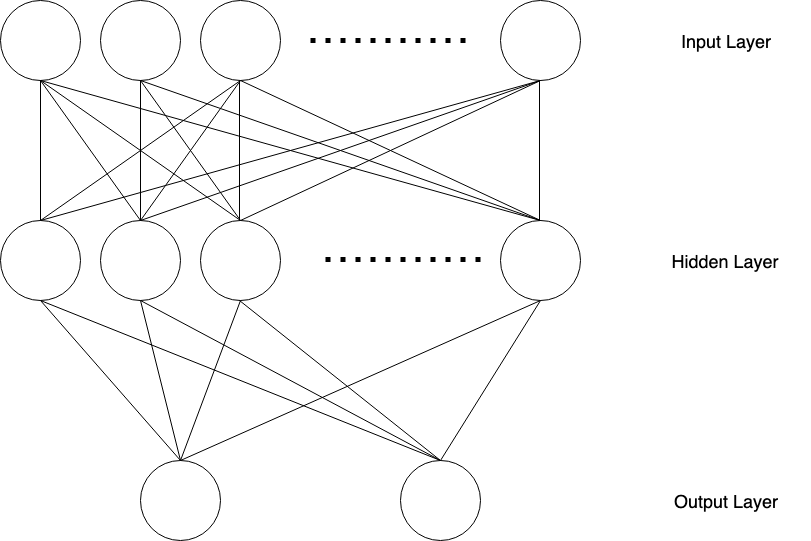
\includegraphics[width=\textwidth]{figures/MSNNfu.png}
  \caption{Schematic of a multilayerd SNN with two output neurons}
  \label{fig:MSNNfull}
\end{figure}
With $r_{l/r}$ as the reward for the left/right neuron and $w_{l/r}$ the connection for this neuron to the left/right output \autoref{eq:rewardProp} simplifies to
\begin{equation}
r_h = \frac{ r_l * w_l + r_r * w_r} {max(|w_l|,|w_r|)*2}
\end{equation}
As the reward defined in \autoref{eq:reward} has the same value with opposing signing the last equation resolves to
\begin{equation}\label{eq:rewardPSimp}
r_h = \frac{ -r_r * w_l + r_r * w_r} {max(|w_l|,|w_r|)*2}
\end{equation}
\begin{equation*}
  r_h = \frac{ r_r *(w_r-w_l) } {max(|w_l|,|w_r|)*2}
\end{equation*}
In this manner the reward for each neuron can be calculated.

% !TeX root = ../main.tex
% Add the above to each chapter to make compiling the PDF easier in some editors.

\chapter{Training}\label{chapter:Training}
This chapter first describes the default setup of the network and the training task. Followed by the specification of the target and its trajectory. Afterwards the specifics of the different experiment setups are described as well as the results of the training phase.
\section{Structure and parameters of the network}
In this thesis SNNs in different topologies as well as with different parameter settings are going to be tested. First the simplest topology is used consisting of ten poisson neurons, ten LIF input neurons and two LIF output neurons with each a spike detector connected. \autoref{fig:simpleNetwork} shows a schematic of the network where all but the connections between the input and hidden are static and only between the LIF neurons R-STDP synapses are used. The input layer of LIF neurons are set up to parrot the spikes from the poisson neurons and is necessary as the poisson layer is defined by the transfer functions and thus connections to it can not be described in the simulation setup of the network. To produce this behaviour of the neurons their refractory period is set to zero and their threshold voltage is set close to the resting voltage. The exact parameters are shown in \autoref{tab:parrotPar}.


\begin{figure}[htpb]
  \centering
  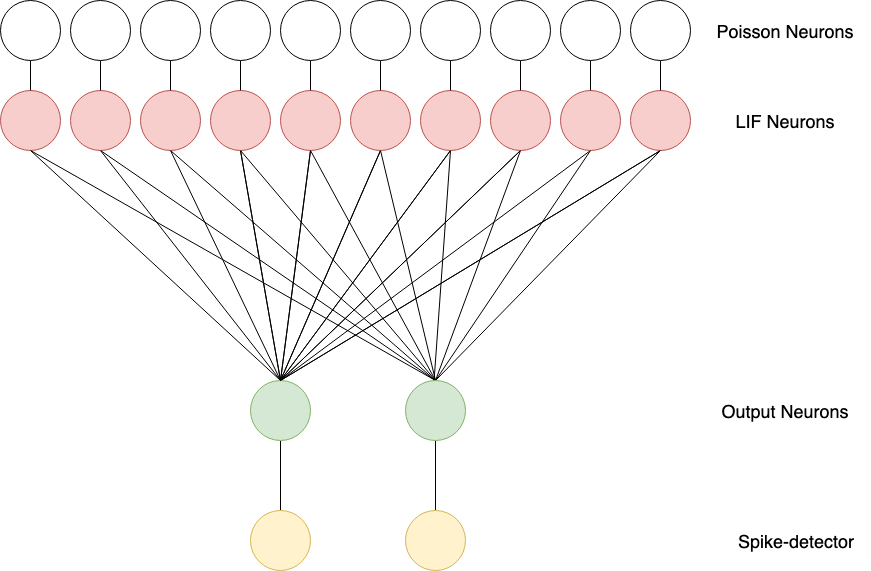
\includegraphics[width=\textwidth]{figures/plots/simpleNetwork}
  \caption Simple Network]{This figure shows the Simplest Network Topology used for simulations}
  \label{fig:simpleNetwork}
\end{figure}

\begin{table}[htpb]
\caption[Parameters Parrot Neuron]{Parameters of Parrot Neurons} \label{tab:parrotPar}
\centering
\begin{tabular}{|c| c |l|}
    \toprule
    Parameter & Value & Description \\
    \midrule
    $c_m$   & 1.0  & Capacity of the membrane \\
    $tau_{m}$    & 20.0  & Membrane time constant \\
    $tau_{refrac}$   & 0.  & Duration of refractory period\\
    $v_{thresh}$   & -64.50  & Spike initiation threshold \\
    $v_{reset}$    & -65.0  &  Reset value for $V_m$ after a spike \\
		$v_{rest}$ & -65.0 & Resting voltage \\
    \bottomrule
\end{tabular}
\end{table}

In the output layer the parameters are set to get a behaviour where some spikes are needed to fire the neuron but it still doesn’t fire to sparse. This behaviour is wanted as it somehow defines basic requirements for learning. Are the spikes to rare the synapses connecting to it won’t learn, on the other hand if the neuron fires with every incoming spike the ability to learn is at least strongly hindered as it makes the eligibility mechanism useless. To reduce the impact of a single spike on the potential of the neuron, its capacity can be increased while the time window in which these spikes can appear can be spread by increasing the membrane time constant. The parameters used for the output layer can be seen in \autoref{tab:outputParam}.


\begin{table}[htpb]
  \caption[Parameters Output Neuron]{Parameters of Output Neurons} \label{tab:outputParam}
  \centering
  \begin{tabular}{|c| c |l|}
      \toprule
      Parameter & Value & Description \\
      \midrule
      $c_m$   & 10.0  & Capacity of the membrane \\
      $tau_{m}$    & 50.0  & Membrane time constant \\
      $tau_{refrac}$   & 1.  & Duration of refractory period\\
      $v_{thresh}$   & -50.0  & Spike initiation threshold \\
      $v_{reset}$    & -65.0  &  Reset value for $V_m$ after a spike \\
      $v_{rest}$ & -65.0 & Resting voltage for $V_m$ \\
      \bottomrule
  \end{tabular}
  \end{table}

The parameters for the R-STDP synapses are shown in \autoref{tab:baseRstdp} and are chosen to have only a short memory to the past and a balanced eligibility for the STDP learning windows. The memory timespan is proportional to he eligibility time constant $\tau_c$ which is set to $40$ milliseconds, two times the simulation timestep. The height of the STDP function for a pre-post-spiking pattern is given by $A_+$ and for a post-pre pattern by $A_-$ which are the constant scaling strengths of potentiation and depression and are set to the same value to have an equal impact on the eligibility trace. To achieve stable learning the change in weights shouldn’t be too extreme as the network is unlikely to stabilise in such a scenario. As \autoref{eq:dWrStdp} shows the weight change is proportional to the magnitude of the eligibility trace $c$ and the neuromodulator concentration $n$. Thus the magnitude of the scaling factors $A_{+/-}$, influencing the magnitude of $c$,  have to be balanced with the scaling factor $c_{rew}$ of the reward function shown in \autoref{eq:reward}, influencing the magnitude of $n$. In this experiments the baseline concentration $b$ in \autoref{eq:dWrStdp} is set to zero as the concentration is directly assigned and not regulated through a dopamine neuron. Thus negative values can be assigned which otherwise would result by a lower neuromodulator concentration $n$ than the baseline concentration $b$.

\begin{table}[htpb]
  \caption[Parameters R-STDP synapse]{Parameters of R-STDP Synapse} \label{tab:baseRstdp}
  \centering
  \begin{tabular}{|c| c |l|}
      \toprule
      Parameter & Value & Description \\
      \midrule
      $W_{max}$ & 6000   & Maximum weight of synapse\\   
      $W_{min}$ & -6000  & Minimum weight of synapse\\   
      $A_{+}$   & 0.1    & Constant scaling strength of potentiation\\   
      $A_{-}$   & -0.1   & Constant scaling strength of depression \\   
      $\tau_c$  & 40.0   & Time constant of eligibility trace \\  
      $\tau_n$  & 20.0   & Time constant of reward signal  \\   
      $b$       & 0.0    & Baseline neuromodulator concentration \\    
      \bottomrule
  \end{tabular}
  \end{table}

The angle used for the reward function, which can be seen as the target angle to minimize, is the angle of the head to the ball at each timestep. Further if this angle overcomes $35$ degrees the target and robot get reset to the starting positions and the path of the target gets inverted.
The reward factor $c_{rew}$ in the \autoref{eq:reward} is set to $0.00005$ and the reward is halved every $3000$ time steps which helps the network to better stabilise over time. Stabilisation means that the weights in the network only change to small degree or at best not at all. For this to happen the reward to the network has to be zero or near to it. For the angle from the snakes head to the ball this is not possible for each timestep as result of the movement of the snake. By reducing the reward over time we negate this effect to some degree. The factor $c_{imp}$ in \autoref{eg:OutputCalc} is set to $0.05$, this is scaling the impact of the networks output on the direction. 

\section{Simulation environment}
For the simulation the robot is placed in an empty environment with a sphere as target which is spawned $1.6$ meters in front of the robot with a radius of $30$ centimeters. The sphere or ball is then moved along a path in an eight shaped form. A schematic of the movement pattern of the ball is shown in \autoref{fig:ballMove}, the directions from one point to the other can be found in \autoref{tab:ballMove} in the appendix.
The target is set to move faster than the snake but won’t move further away from the snake then the initial $1.6$ meters.


\section{Benchmark Experiment}
The previously described setting is used as benchmark or baseline setting for testing the capabilities of the setup. 
The training simulation shows that the network is able to completely solve the task on the third try after $151093$ training steps, $3021.86$ seconds, but still heavily depends on the reward signal. The reliance on reward is visible in the strongly changing weights shown in \autoref{fig:midWBase1}. After completing the second run in inverse direction the training was stopped as the weights seemed to have stabilised as can be seen in \autoref{fig:endWBase1}.

\begin{figure}[htpb]
  \centering
  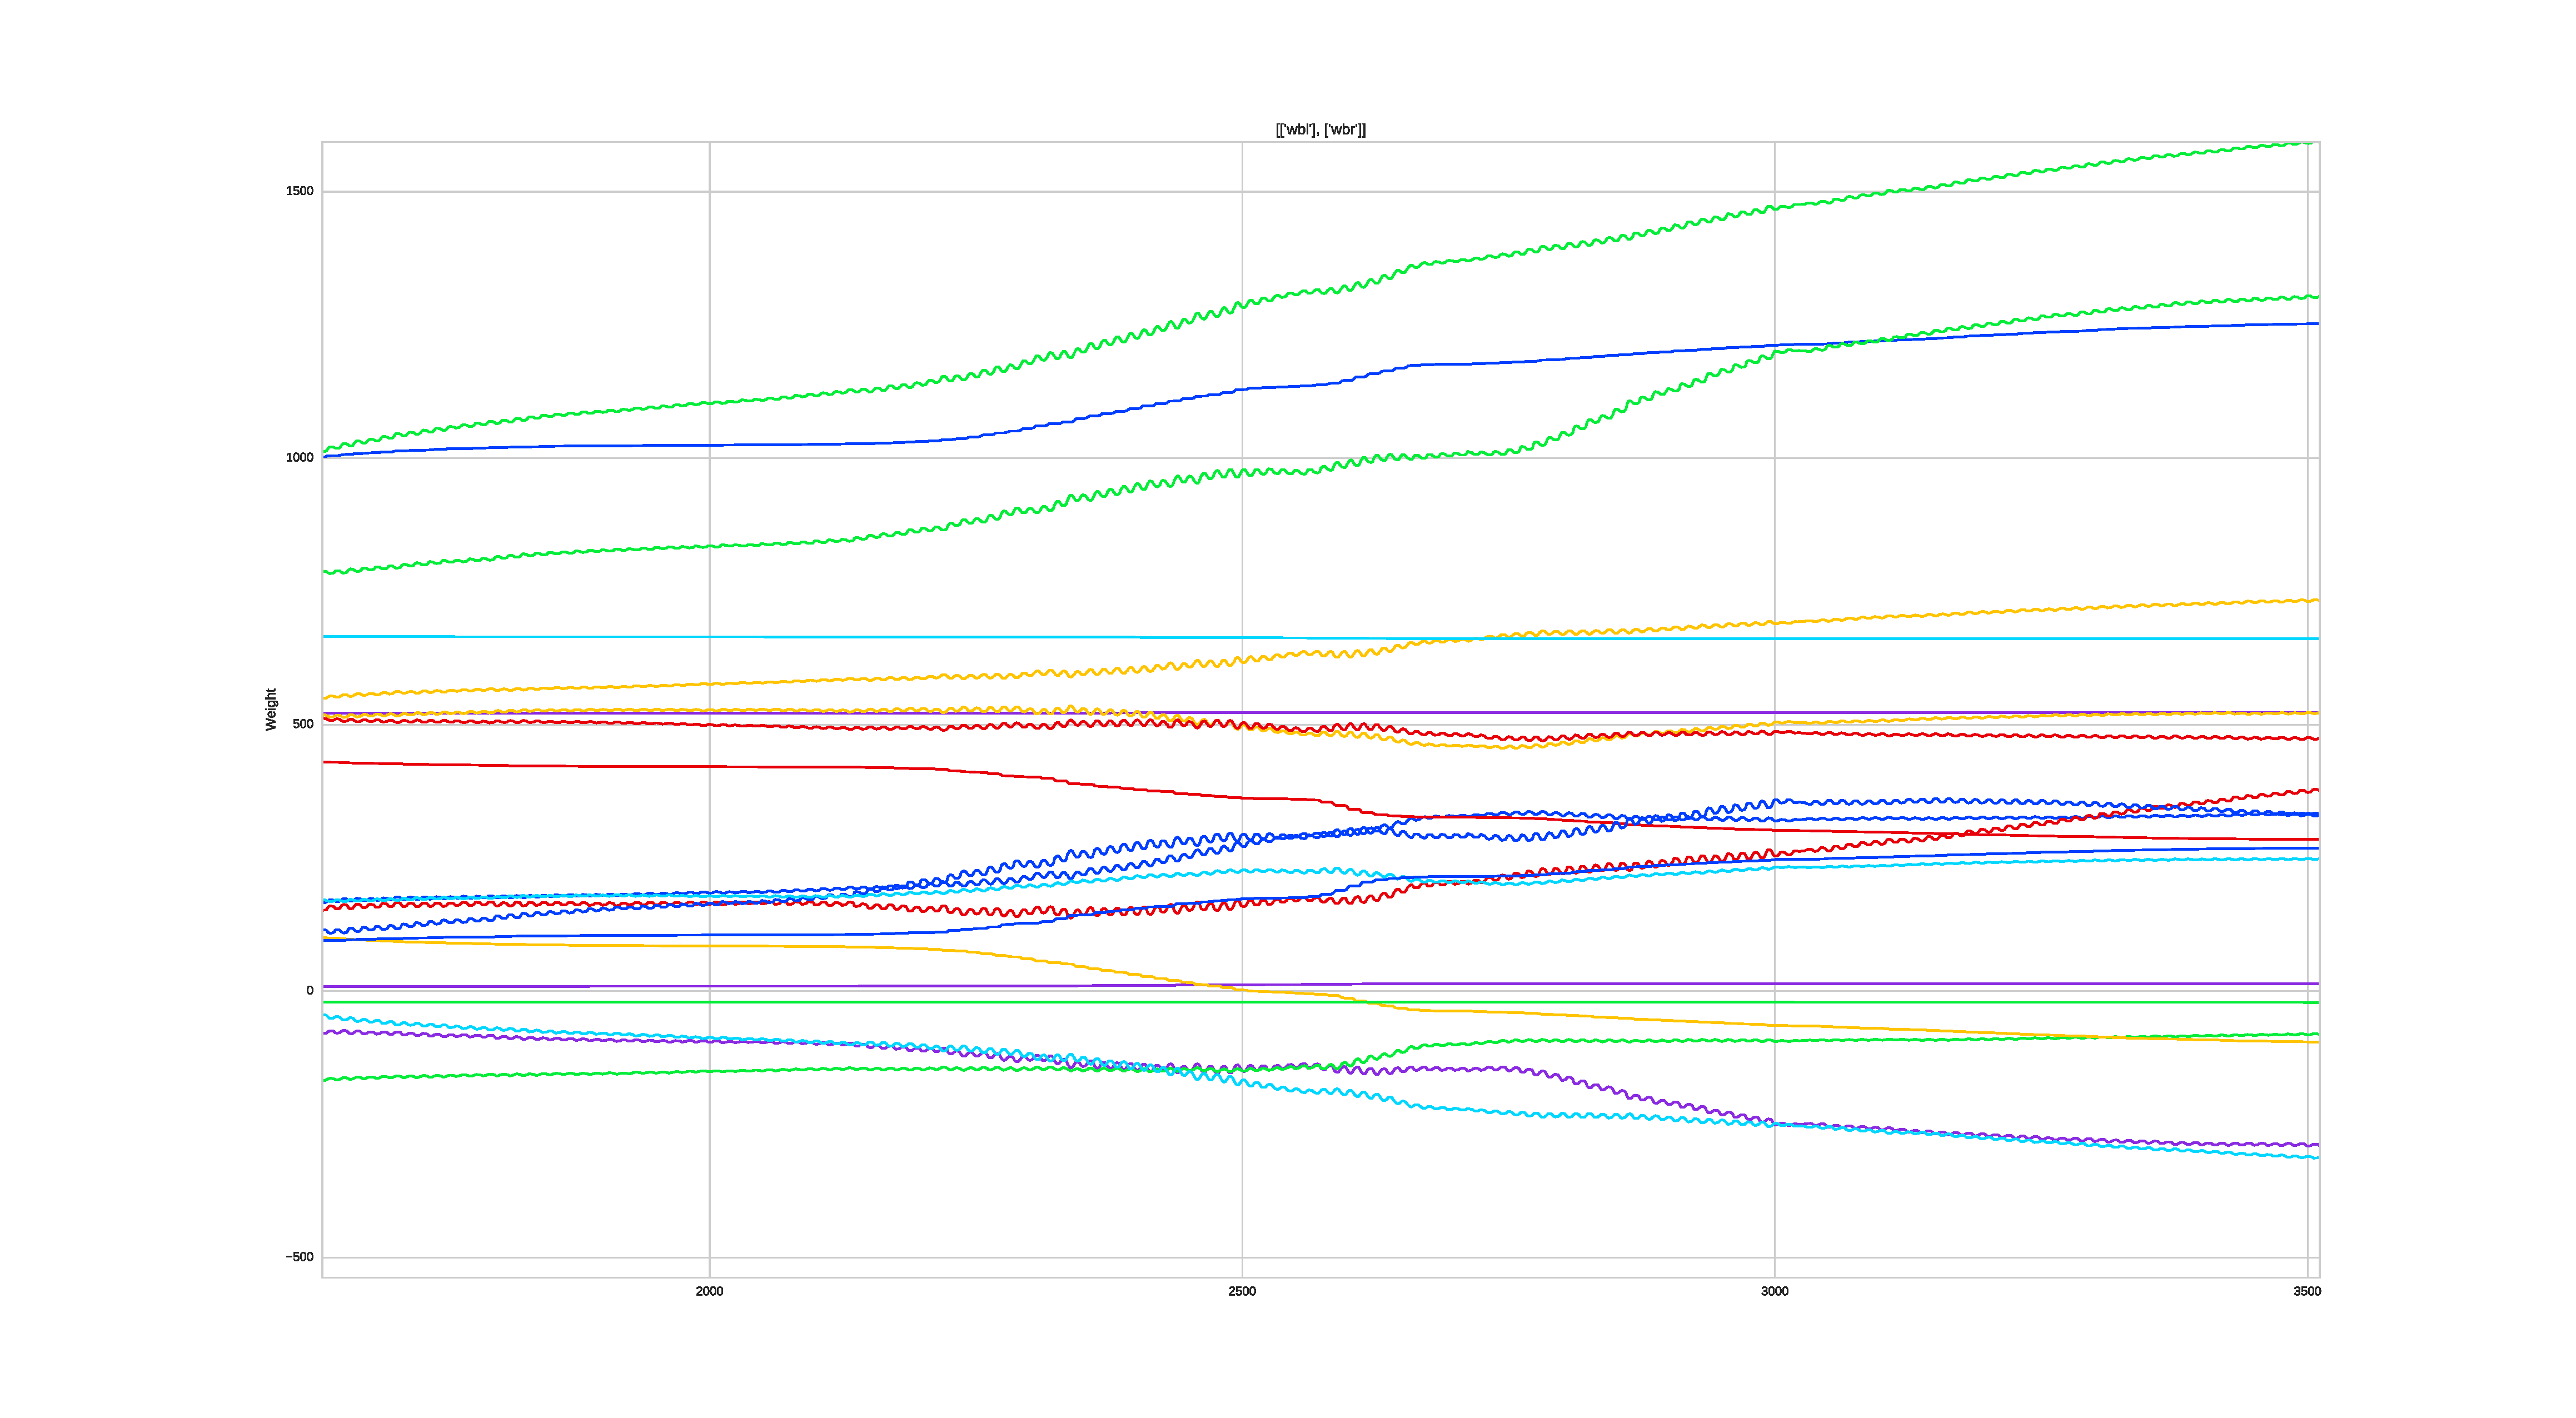
\includegraphics[width=\textwidth]{figures/plots/midWBase1}
  \caption{Movement of weights while still learning }
  \label{fig:midWBase1}
\end{figure}


\begin{figure}[htpb]
  \centering
  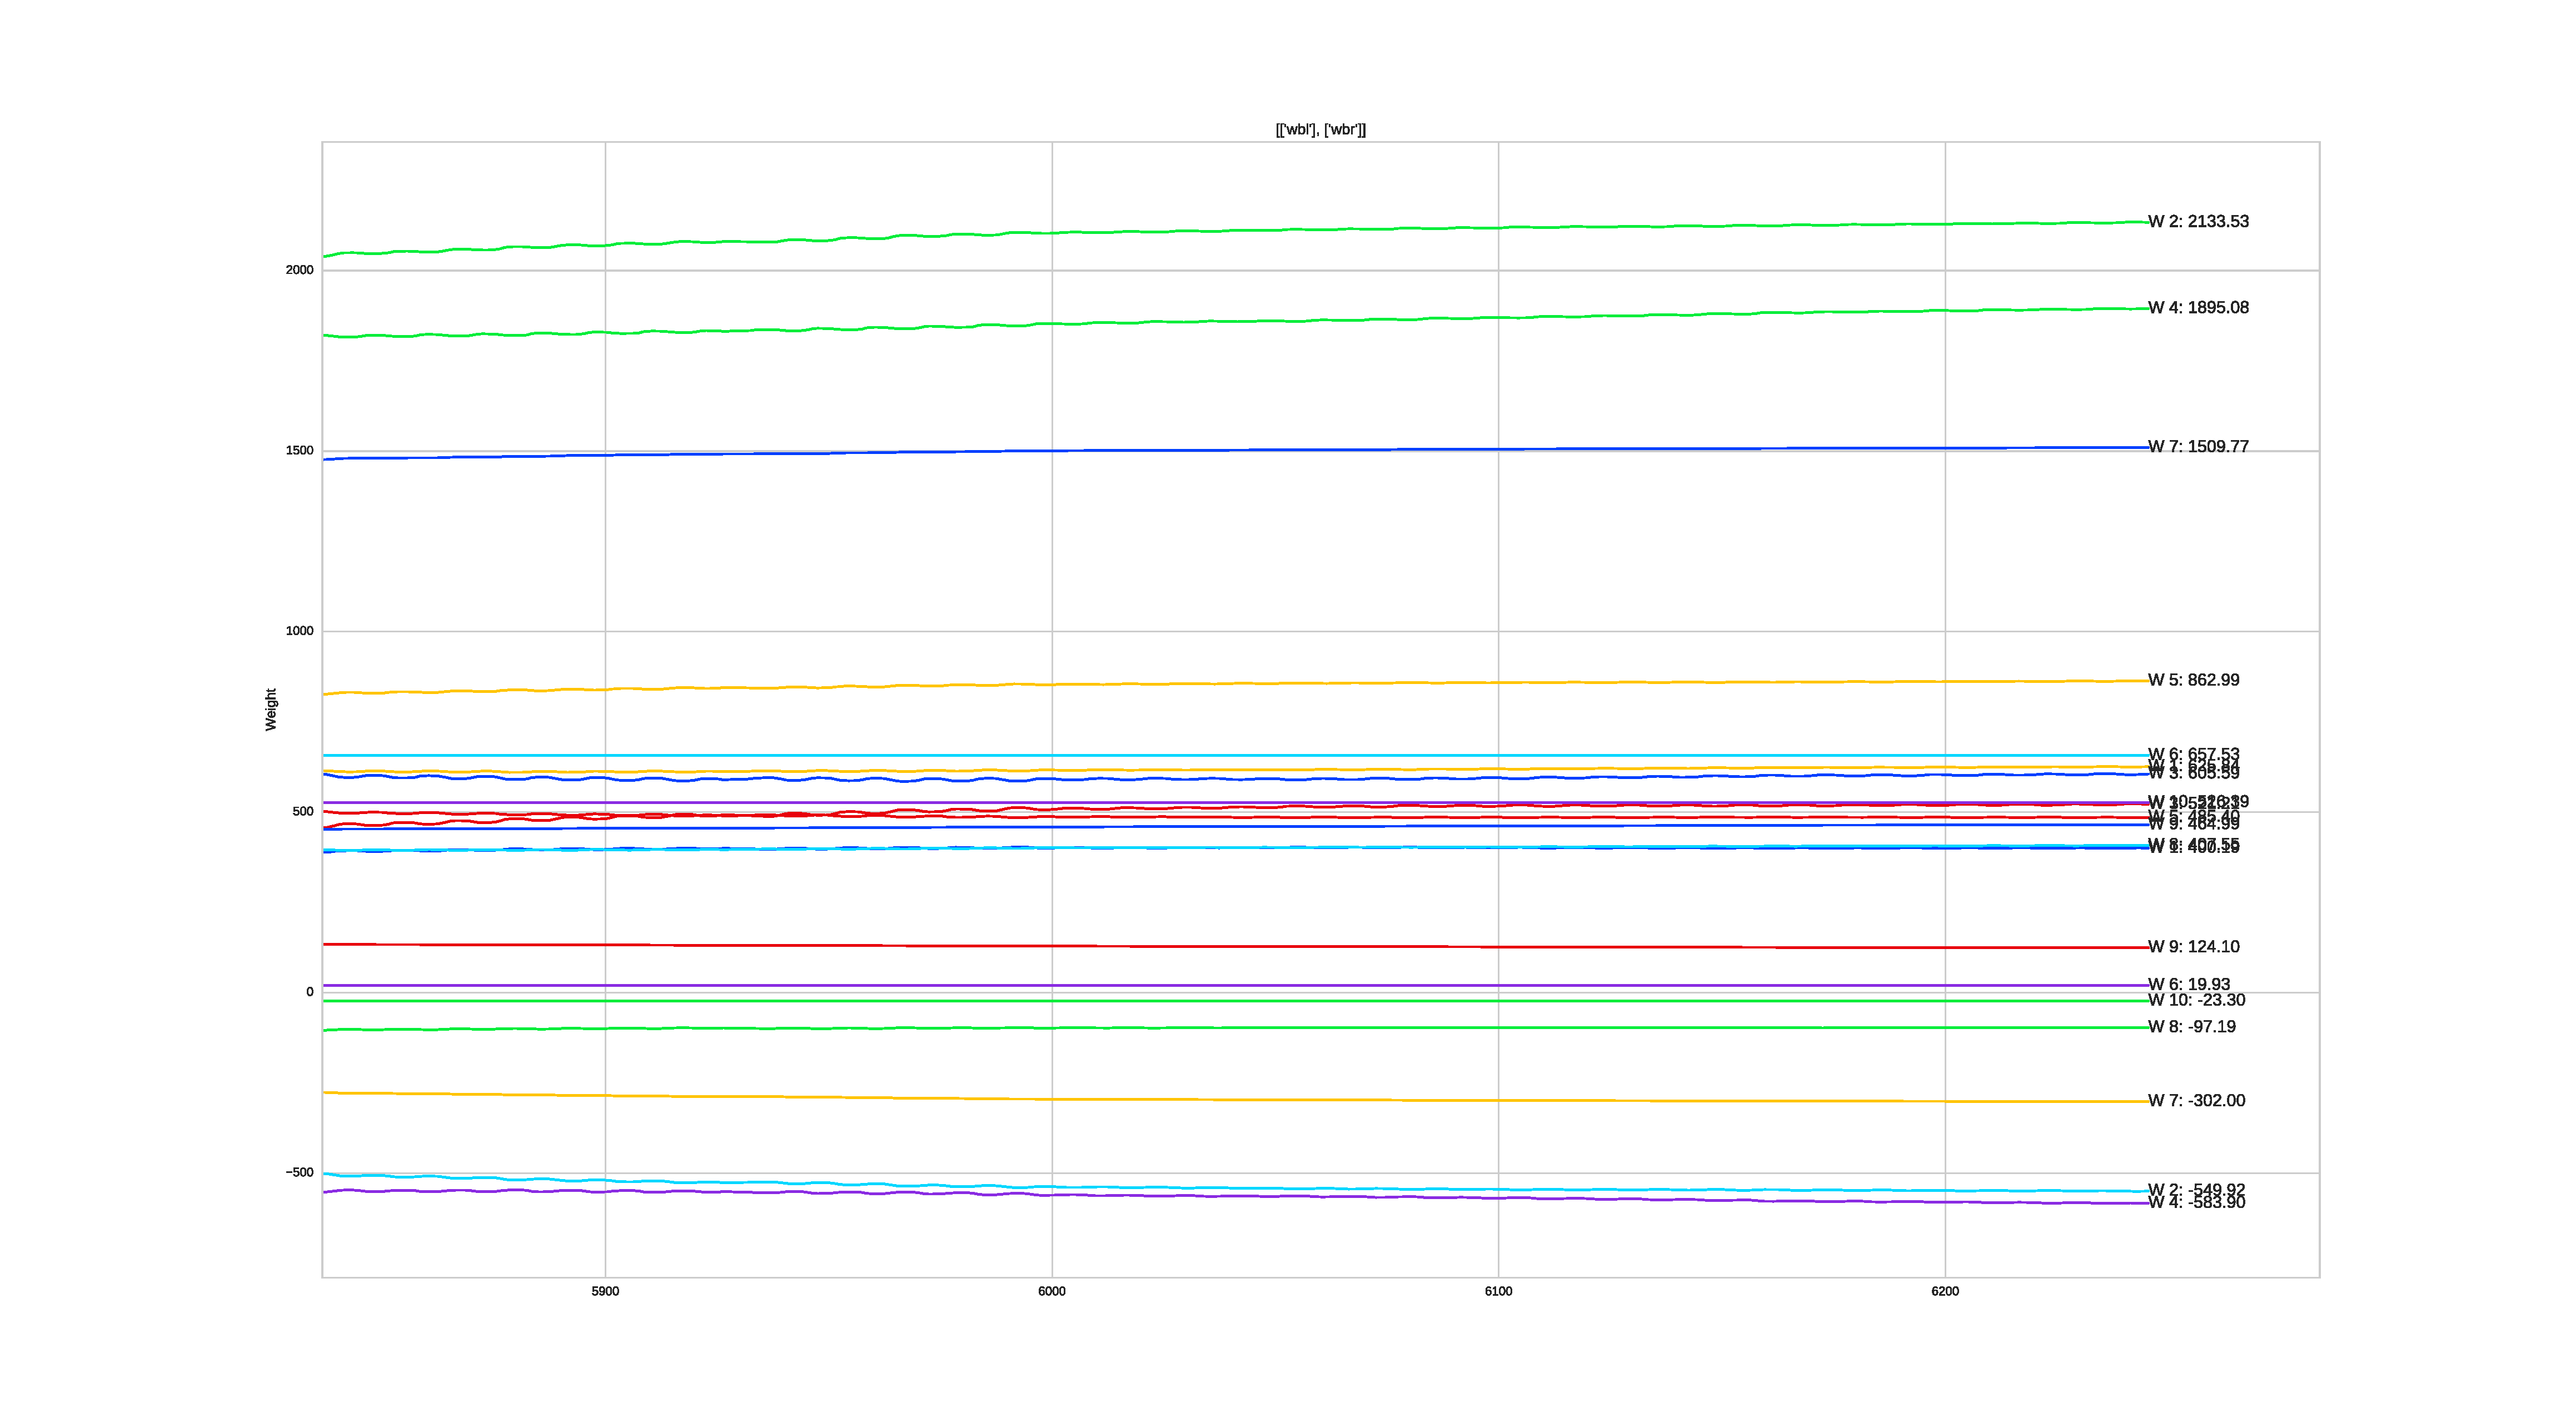
\includegraphics[width=\textwidth]{figures/plots/endWBase1}
  \caption{Movement of weights learning almost ended }
  \label{fig:endWBase1}
\end{figure}
\autoref{fig:WBase1} shows the graph of the weights over the whole training period where \autoref{fig:dopeBase1} and \autoref{fig:angleBase1} show the graphs for reward given to the network and the mean angle and distance to the target over time. \autoref{fig:moveEndBase1} shows the direction the snake took along with the current angle plotted over time for about the last $450$ seconds where the value for the direction is scaled by a factor of $10$.

\begin{figure}[htpb]
  \centering
  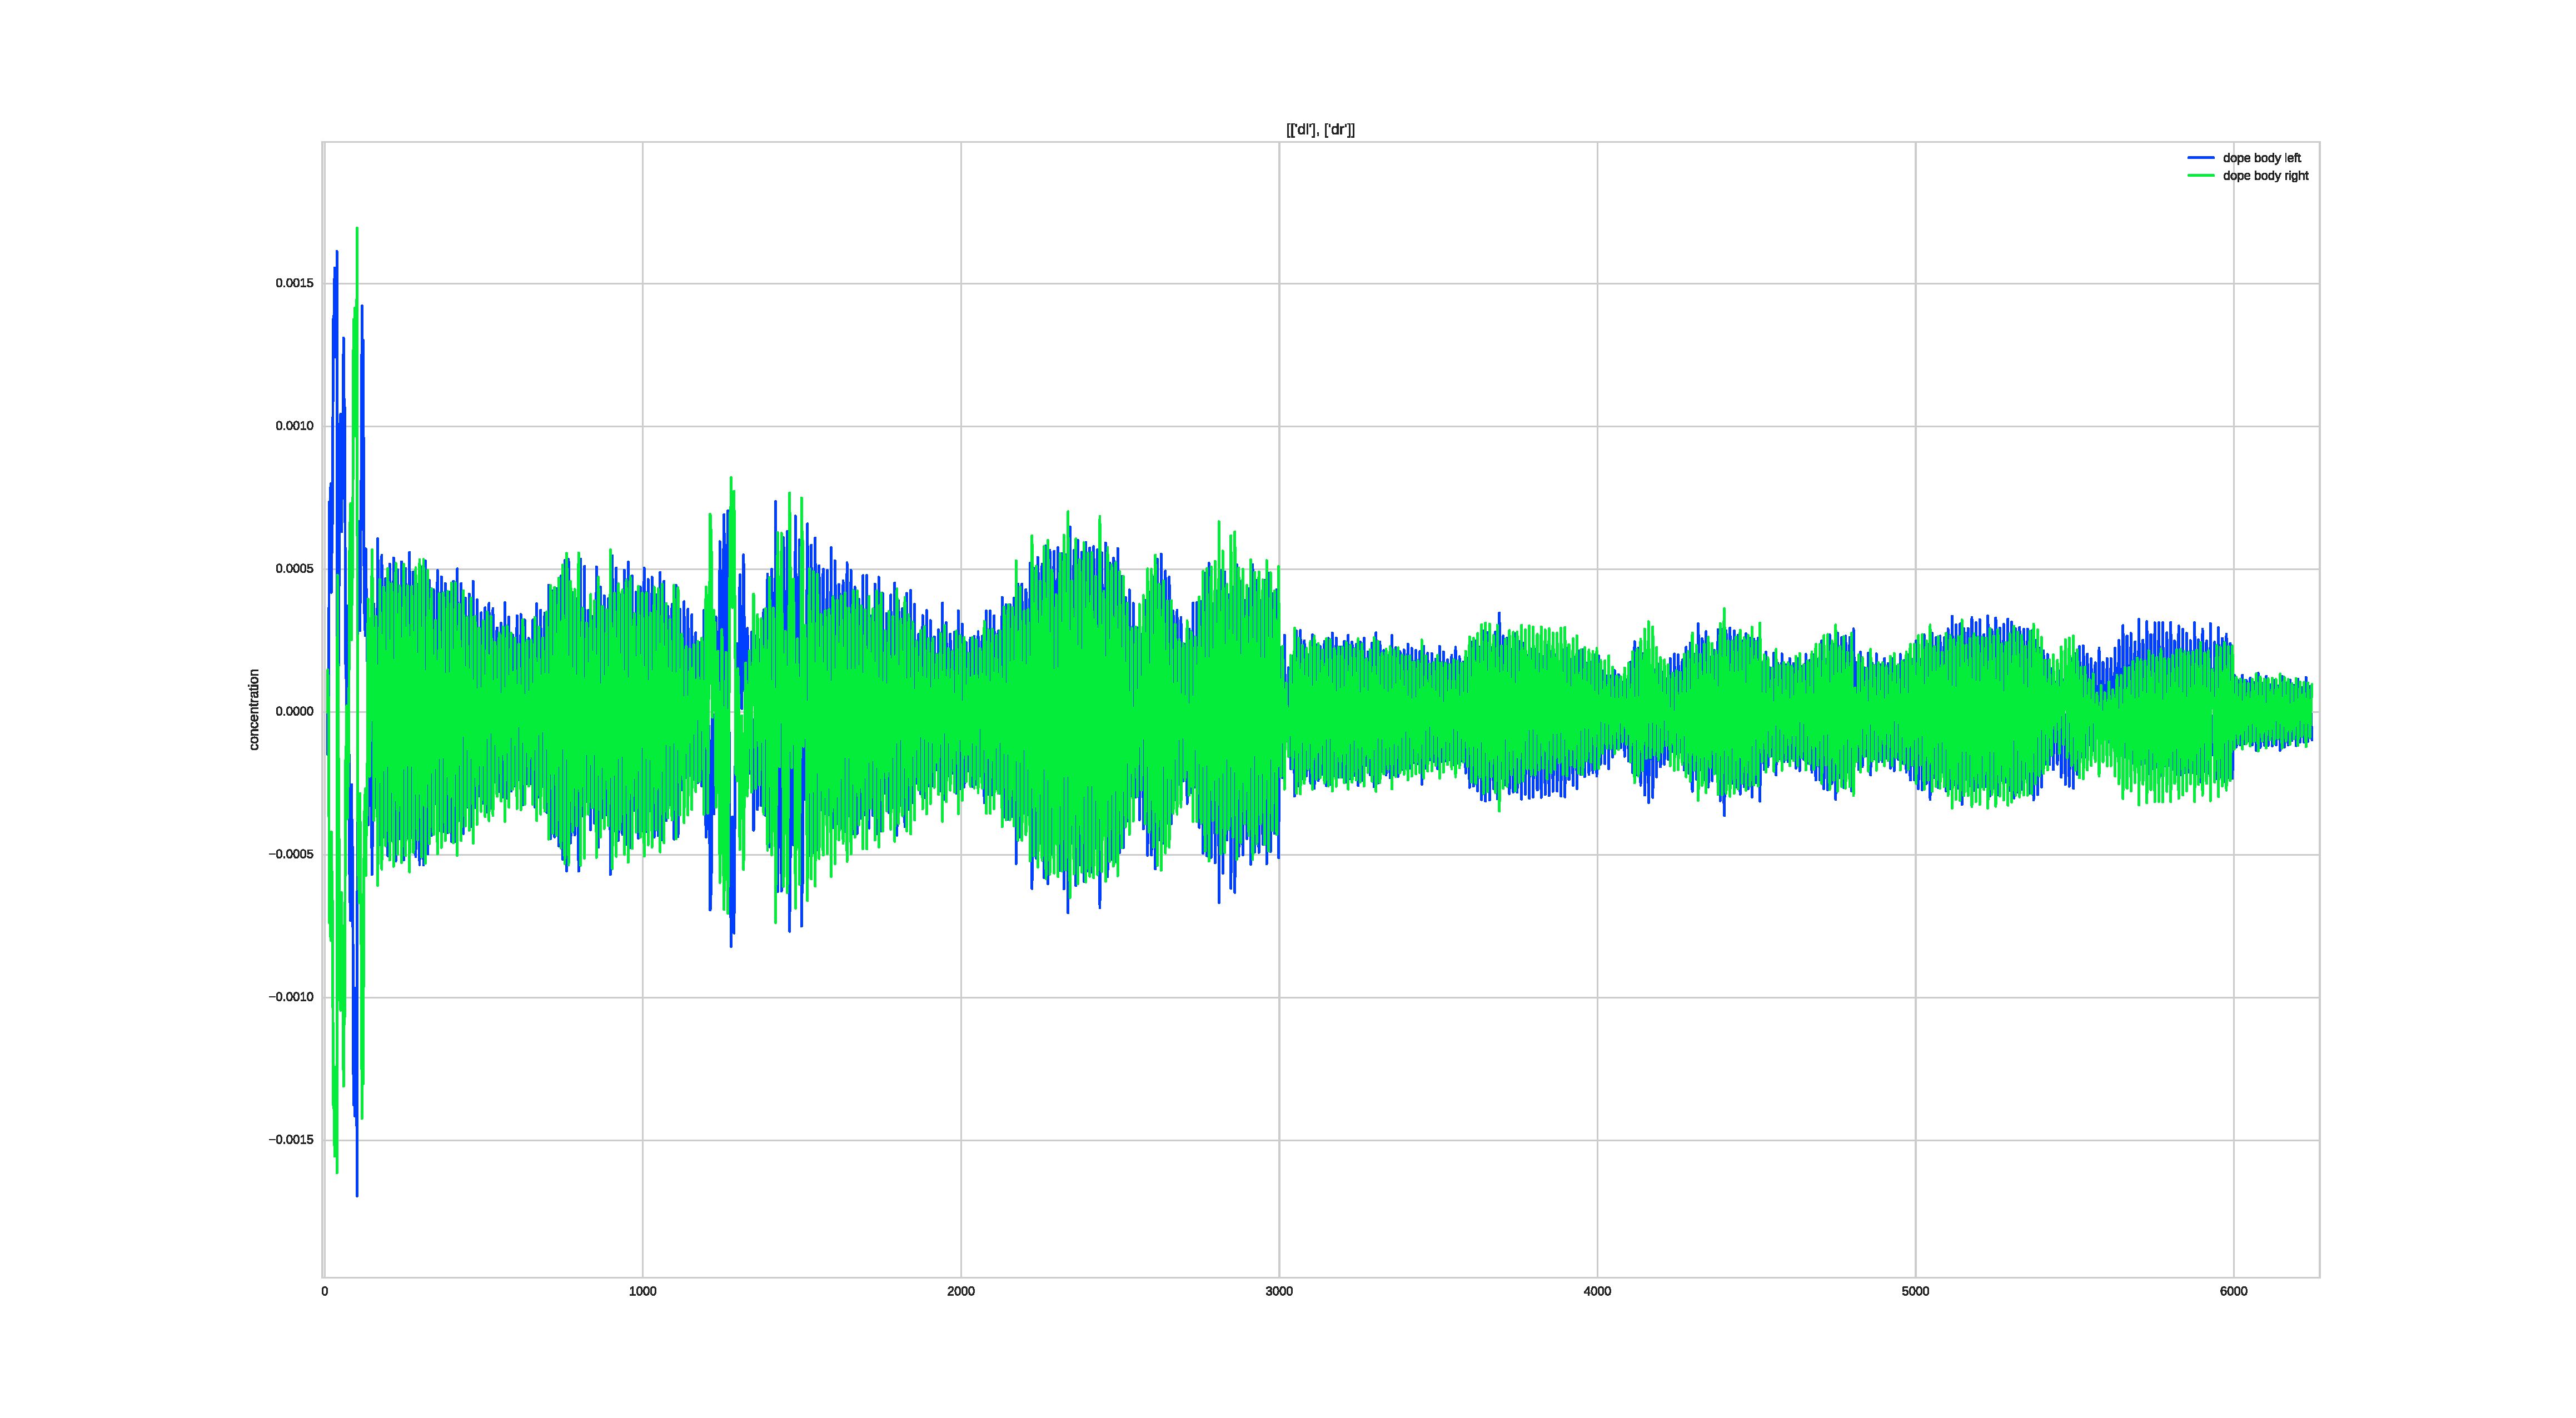
\includegraphics[width=\textwidth]{figures/plots/dopeBase1}
  \caption{ Complete plot of the reward }
  \label{fig:dopeBase1}
\end{figure}
\begin{figure}[htpb]
  \centering
  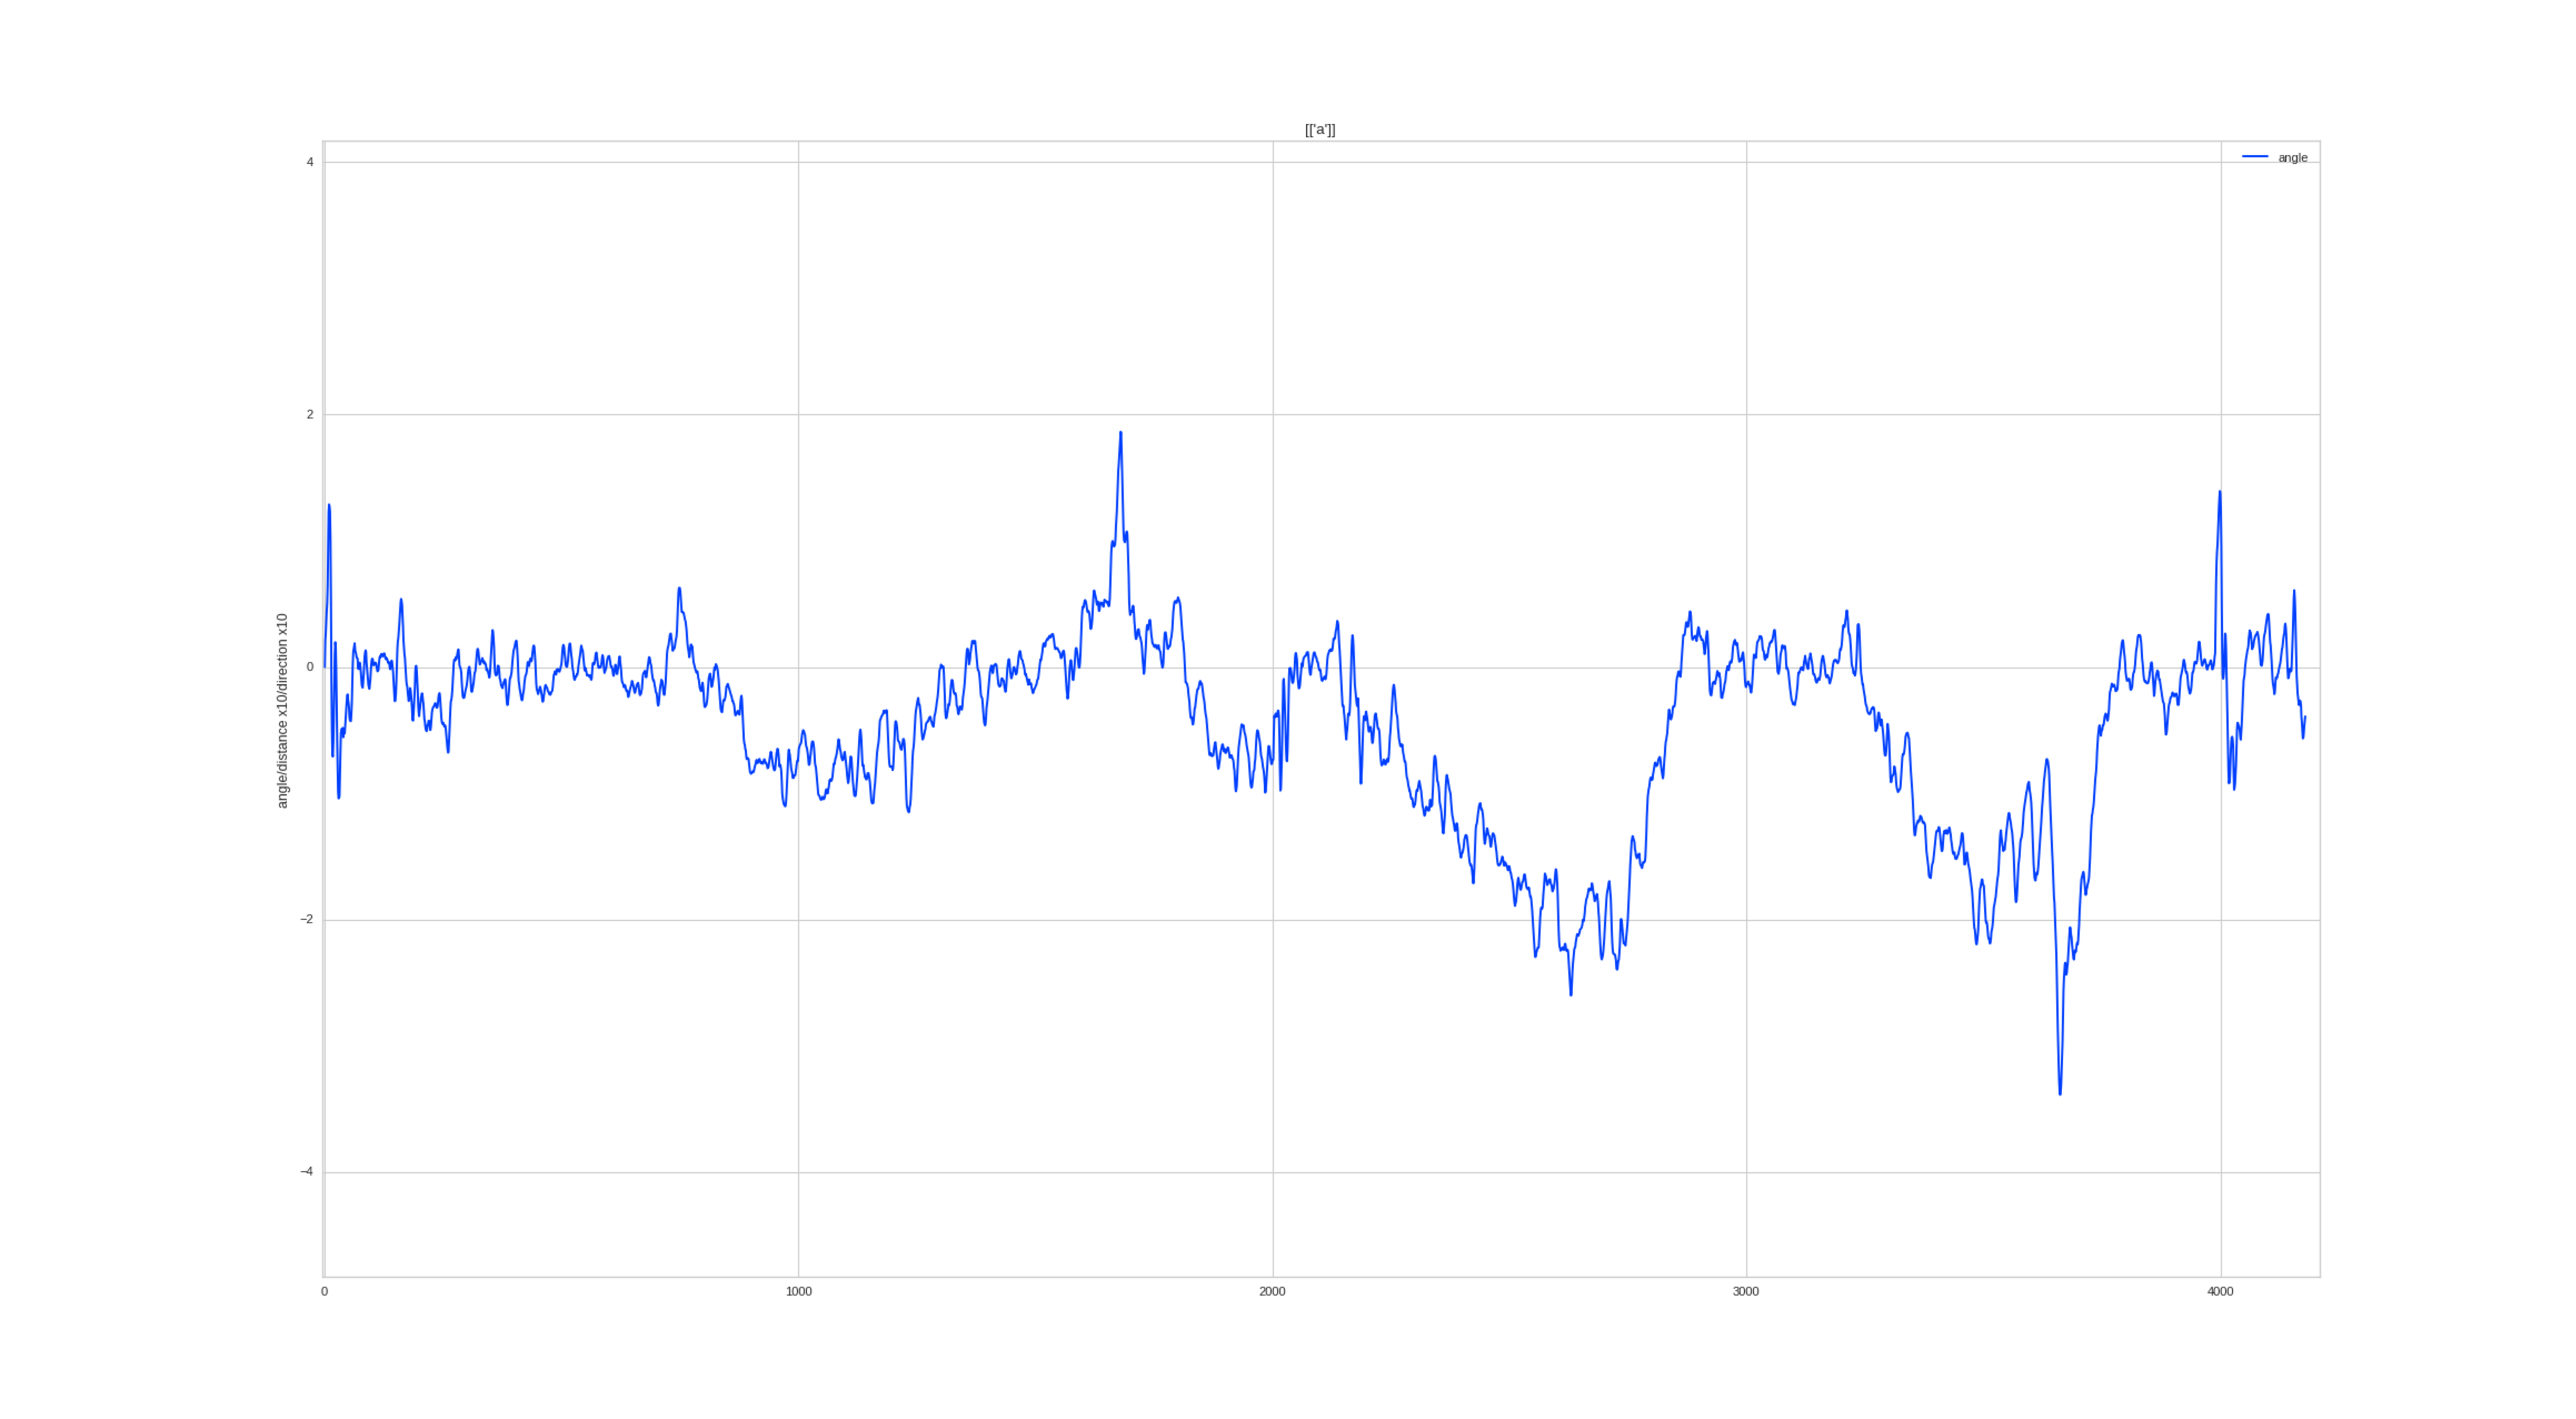
\includegraphics[width=\textwidth]{figures/plots/angleBase1}
  \caption{ Complete plot of the mean angle and distance to the Target }
  \label{fig:angleBase1}
\end{figure}
\begin{figure}[htpb]
  \centering
  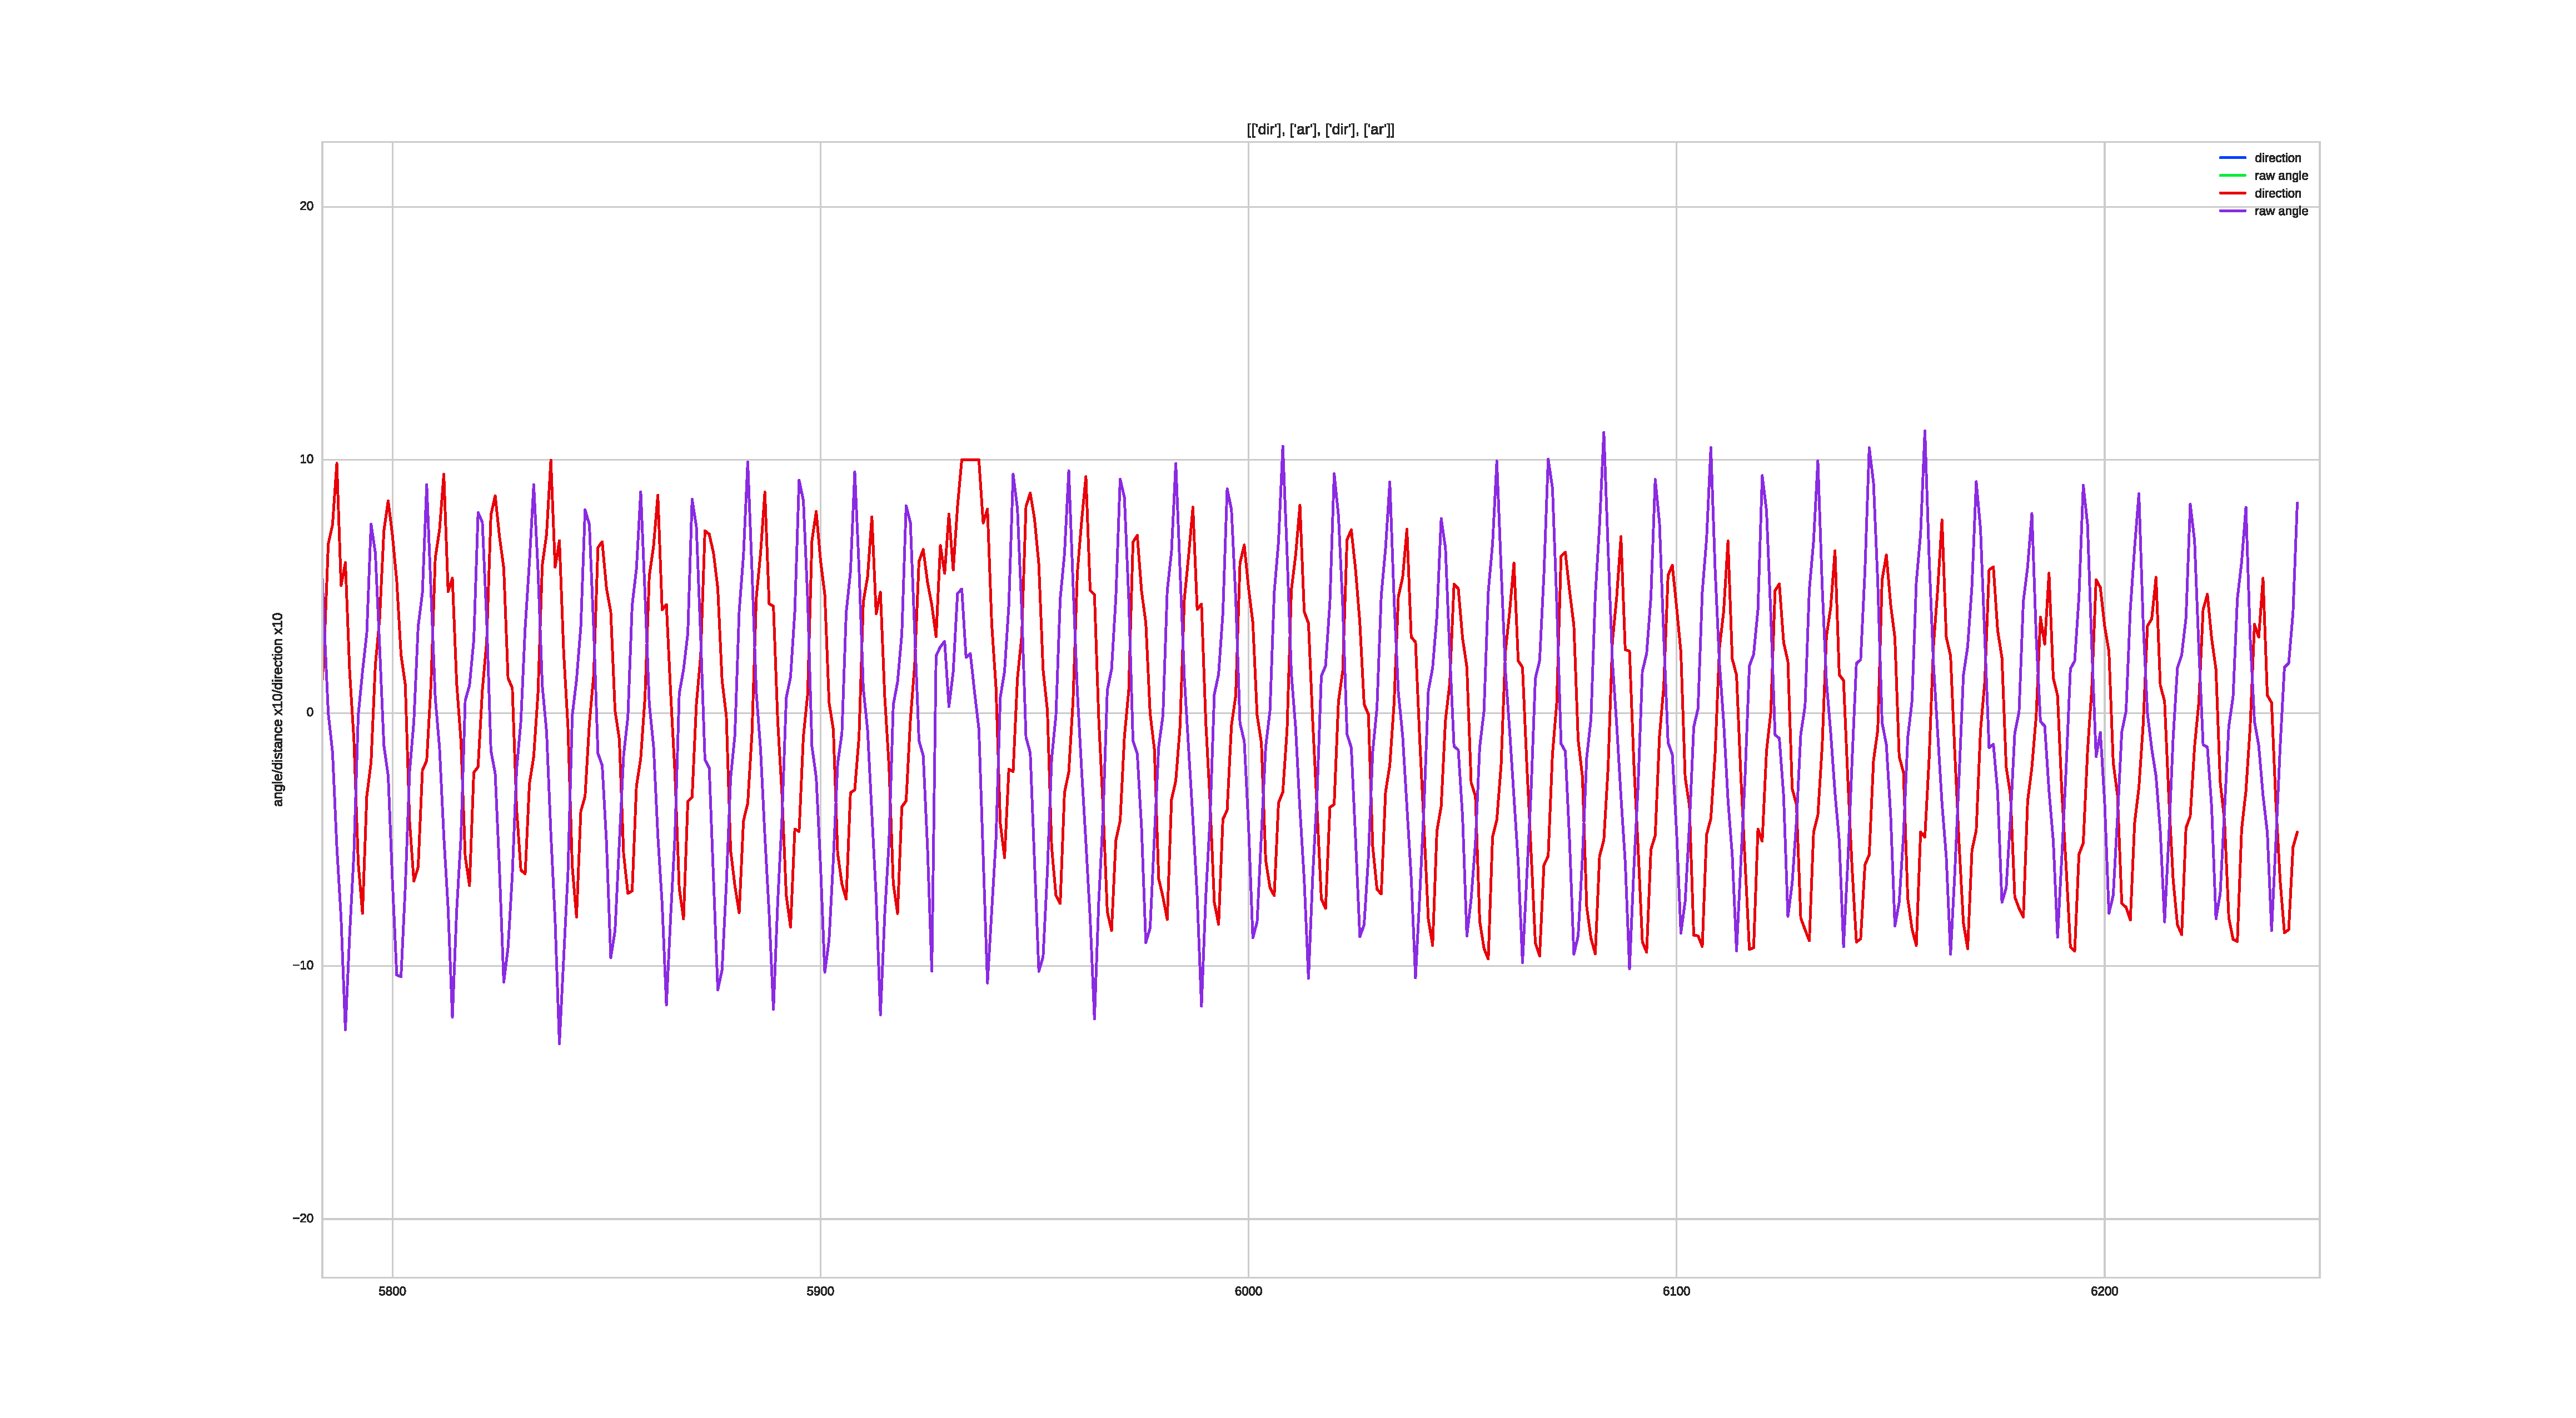
\includegraphics[width=\textwidth]{figures/plots/moveEndBase1}
  \caption{ Plot showing the movement pattern of the Network at the end of the training }
  \label{fig:moveEndBase1}
\end{figure}
\begin{figure}[htpb]
  \centering
  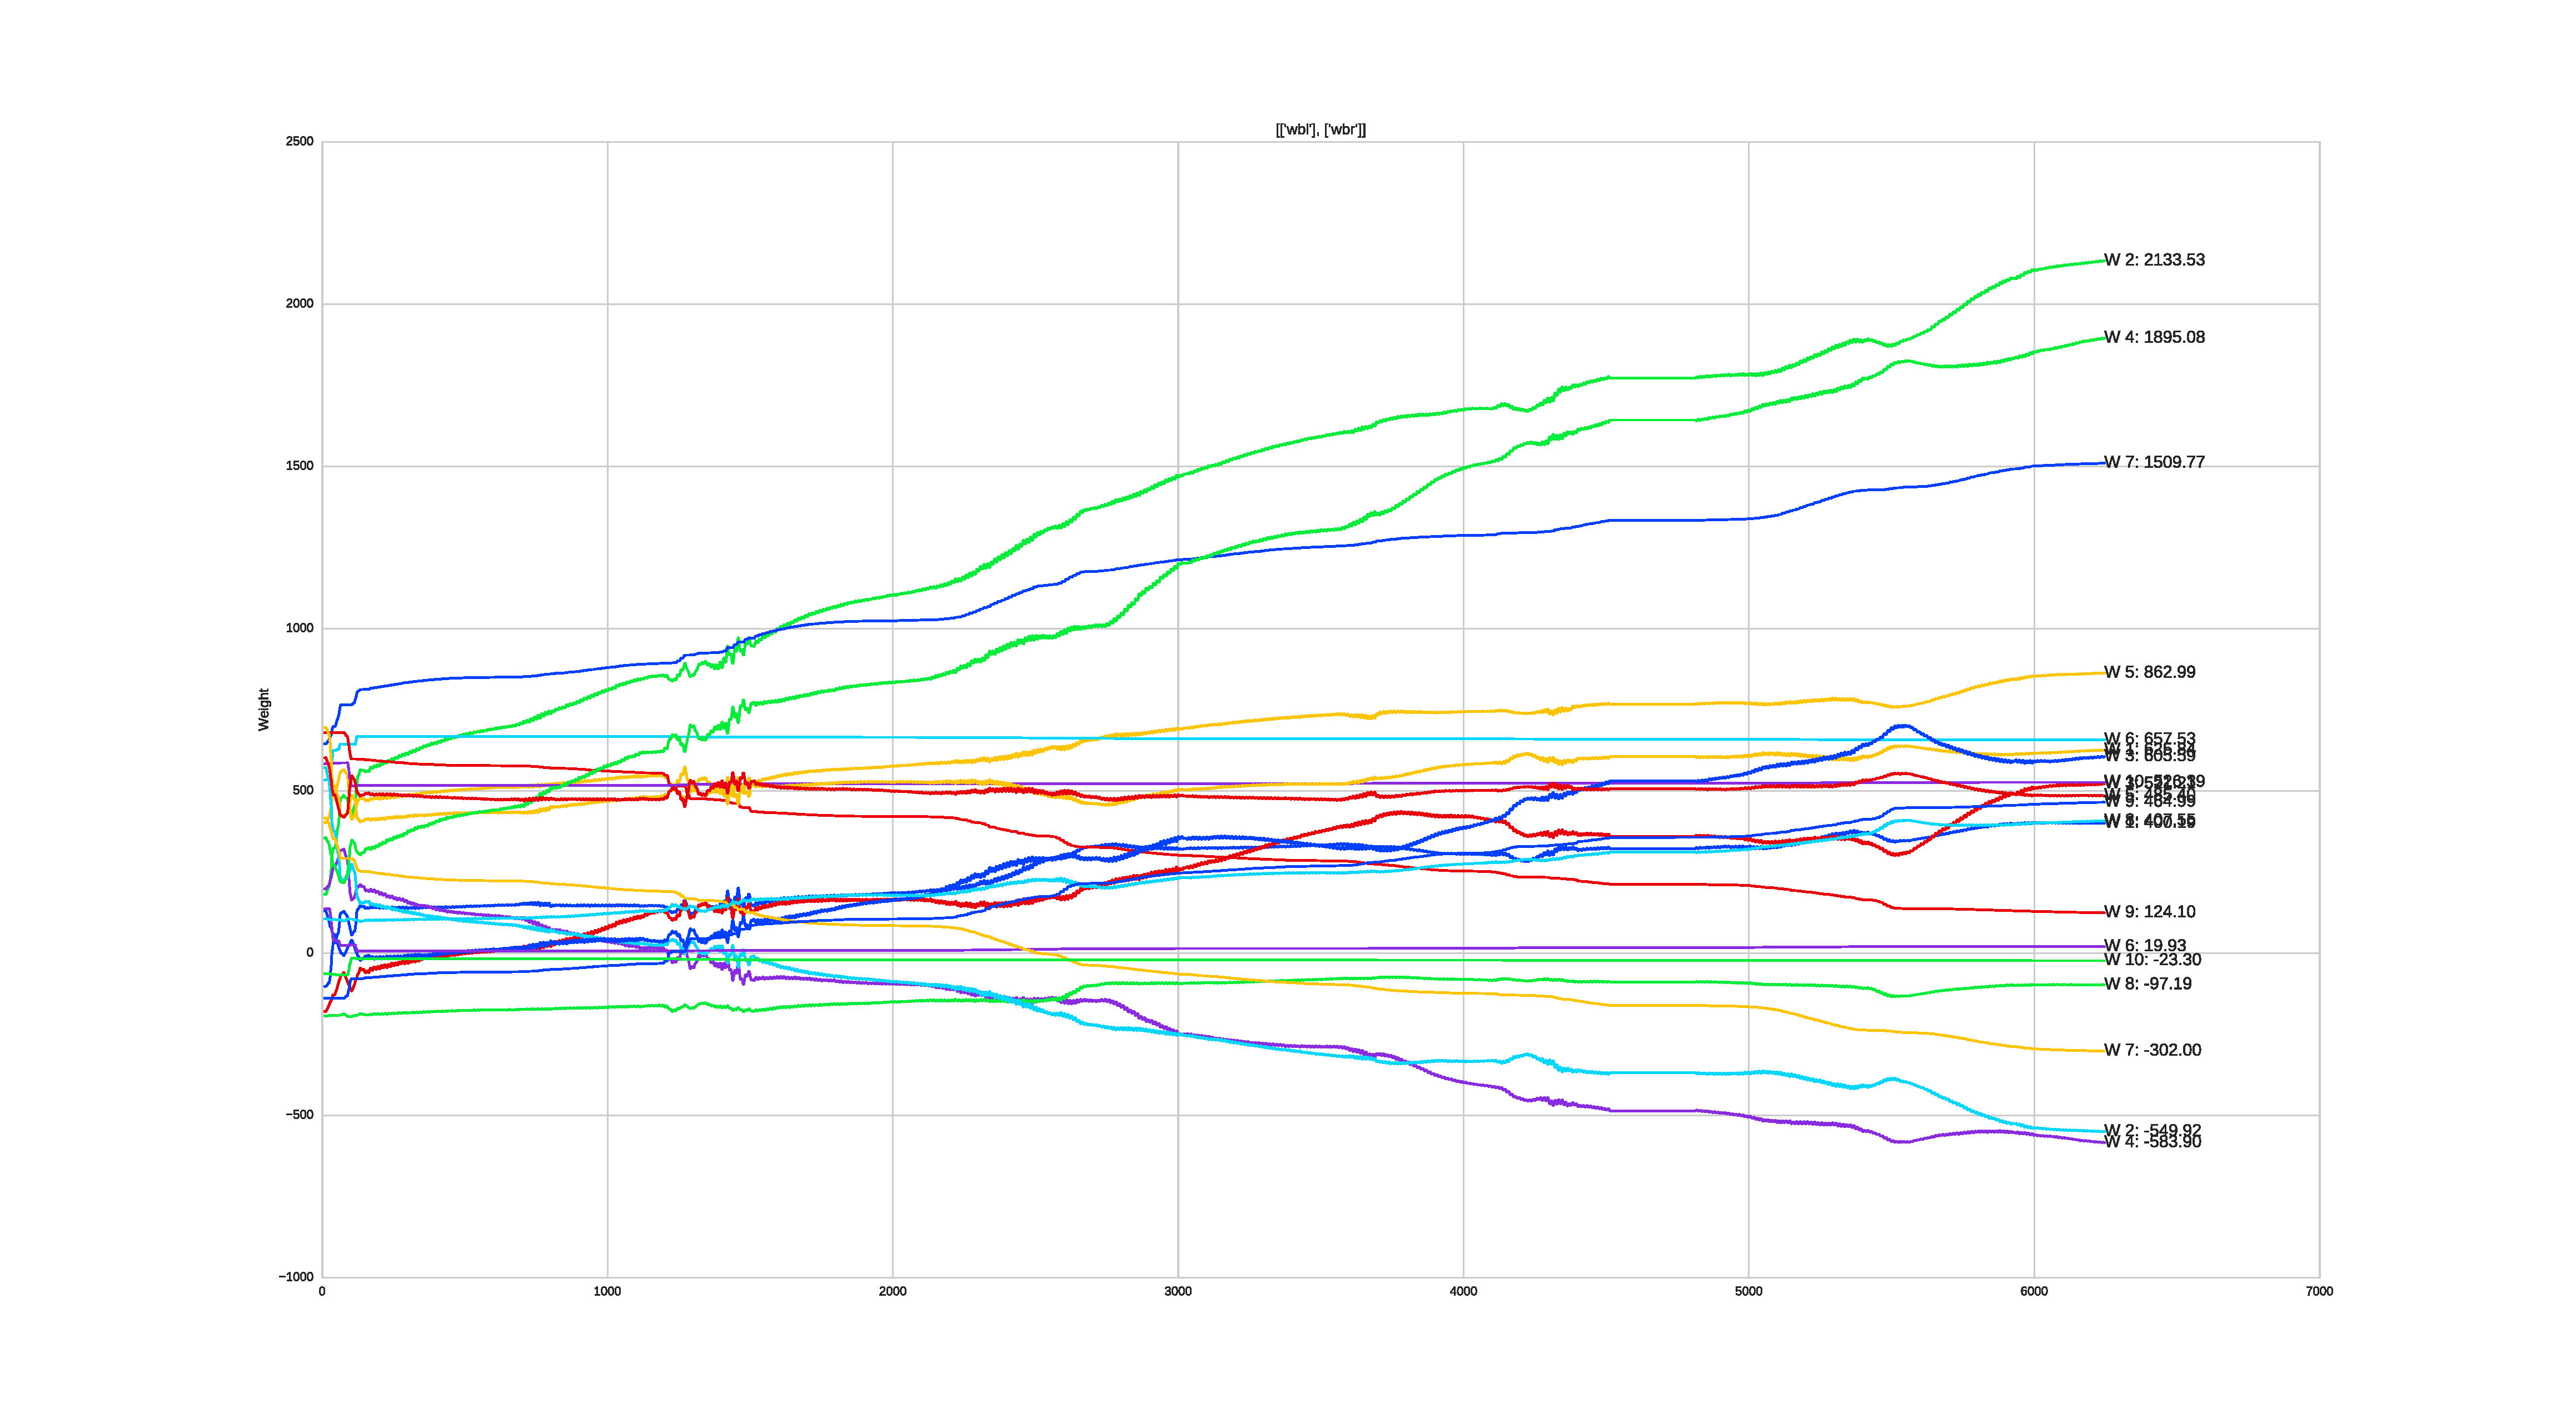
\includegraphics[width=\textwidth]{figures/plots/WBase1}
  \caption{ Complete plot of the weights for the base simulation }
  \label{fig:WBase1}
\end{figure}

\section{Single Layer Network with Head Control}
As follow up task, the network should control the robot direction and additionally the direction the head of the snake is facing. To control the head an additional pair of output neurons is added steering the head in a similar fashion to the other two neurons, described in \autoref{sec:OutputDecoding}. For this setup the factors scaling the impact of the output on the directions in the \autoref{eg:OutputCalc} are set to 0.02 for the head and $0.07$ for the body.
The reward assigned to the neurons controlling the head is as before corresponding to the angle of the head to the target, $a_{head}$, at each timestep. For the body the reward is proportional to the angle of the body to the target $a_{body}$ which is calculated by
\begin{equation} \label{eq:bodyAngle}
a_{body} = a_{head} - d_{head}
\end{equation}
where $d_{head}$ is the direction of the head at that point. This is the angle the snake head would have if it would always face forward.
In this simulation the robot gets reset if the absolute value of either $a_{head}$ is bigger than $40$ degrees or the mean angle of the body is greater than $35$ degrees.
The mean value of the angle is calculated over the past $625$ simulation steps which corresponds to $12.5$ seconds which is the length of one movement period of the snake, meaning in $12.5$ seconds the head will move from one end to the other and back. 
\begin{equation}
A_{mean} = \frac { \sum_{i=0}^{625} a_{t-i} } {625} \text{ ,with $a_{t-i}$ the angle at the $t-i$ timesteps }
\end{equation}
The factor the reward is scaled with $c_{rew}$ is set to $0.0001$ for the body neurons and $0.0004$ for the neurons controlling the head. The other parameters used for the neurons and synapses are shown in \autoref{tab:ParamsBase2N} and \autoref{tab:ParamsBase2S}.

\begin{table}[htpb]
  \centering
  \caption[Parameters 2.Setup]{Parameters of body Neurons in the 2. setup} \label{tab:ParamsBase2N}
  \begin{tabular}{|c| c |l|}
      \toprule
      Parameter & Value & Description \\
      \midrule
      $c_m$   & 20.0  & Capacity of the membrane \\
      $tau_{m}$    & 50.0  & Membrane time constant \\
      $tau_{refrac}$   & 1.  & Duration of refractory period\\
      $v_{thresh}$   & -50.0  & Spike initiation threshold \\
      $v_{reset}$    & -65.0  &  Reset value for $V_m$ after a spike \\
      $v_{rest}$ & -65.0 & Resting voltage for $V_m$ \\
      \bottomrule
    \end{tabular}
    \end{table}
  \begin{table}[htpb]
  \centering
  \caption[Parameters 2.Setup]{Parameters of the body Synapses for the 2. setup} \label{tab:ParamsBase2S}
    \begin{tabular}{|c| c |l|}
        \toprule
        Parameter  & Value & Description \\
        \midrule
        $W_{max}$ & 6000   & Maximum weight of synapse\\   
        $W_{min}$ & -6000  & Minimum weight of synapse\\   
        $A_{+}$   & 0.1    & Constant scaling strength of potentiation\\   
        $A_{-}$   & -0.1   & Constant scaling strength of depression \\   
        $\tau_c$  & 100.0   & Time constant of eligibility trace \\  
        $\tau_n$  & 20.0   & Time constant of reward signal  \\   
        $b$       & 0.0    & Baseline neuromodulator concentration \\    
        \bottomrule
    \end{tabular}
    \end{table}
With the addition of the head control the structure of the network changes only slightly. Previous network is extended by the two new neurons which are as well connected to each input neuron.

\subsection{Dvs input for Body Neurons}
\autoref{fig:perfdvsOnlyB2} shows the performance of the snake, where green is the mean angle of the head, blue the mean angle of the body and read the distance to the ball times ten. It shows that the network performs quite well at the beginning as the reward given to network changes the weights strong enough and the target moves in a straight line away from the snake. Later in the simulation, when the target moves in different angles the network gets more and more unstable as shown in \autoref{fig:wblWbrB2Dvs}. The training was stopped after the robot failing several times shortly after the start of the try. It seems that either the network is not complex enough or the information the network gets is not sufficient to derive the direction the body should take after the input is somewhat stabilised by the head.
\begin{figure}[htpb]
  \centering
  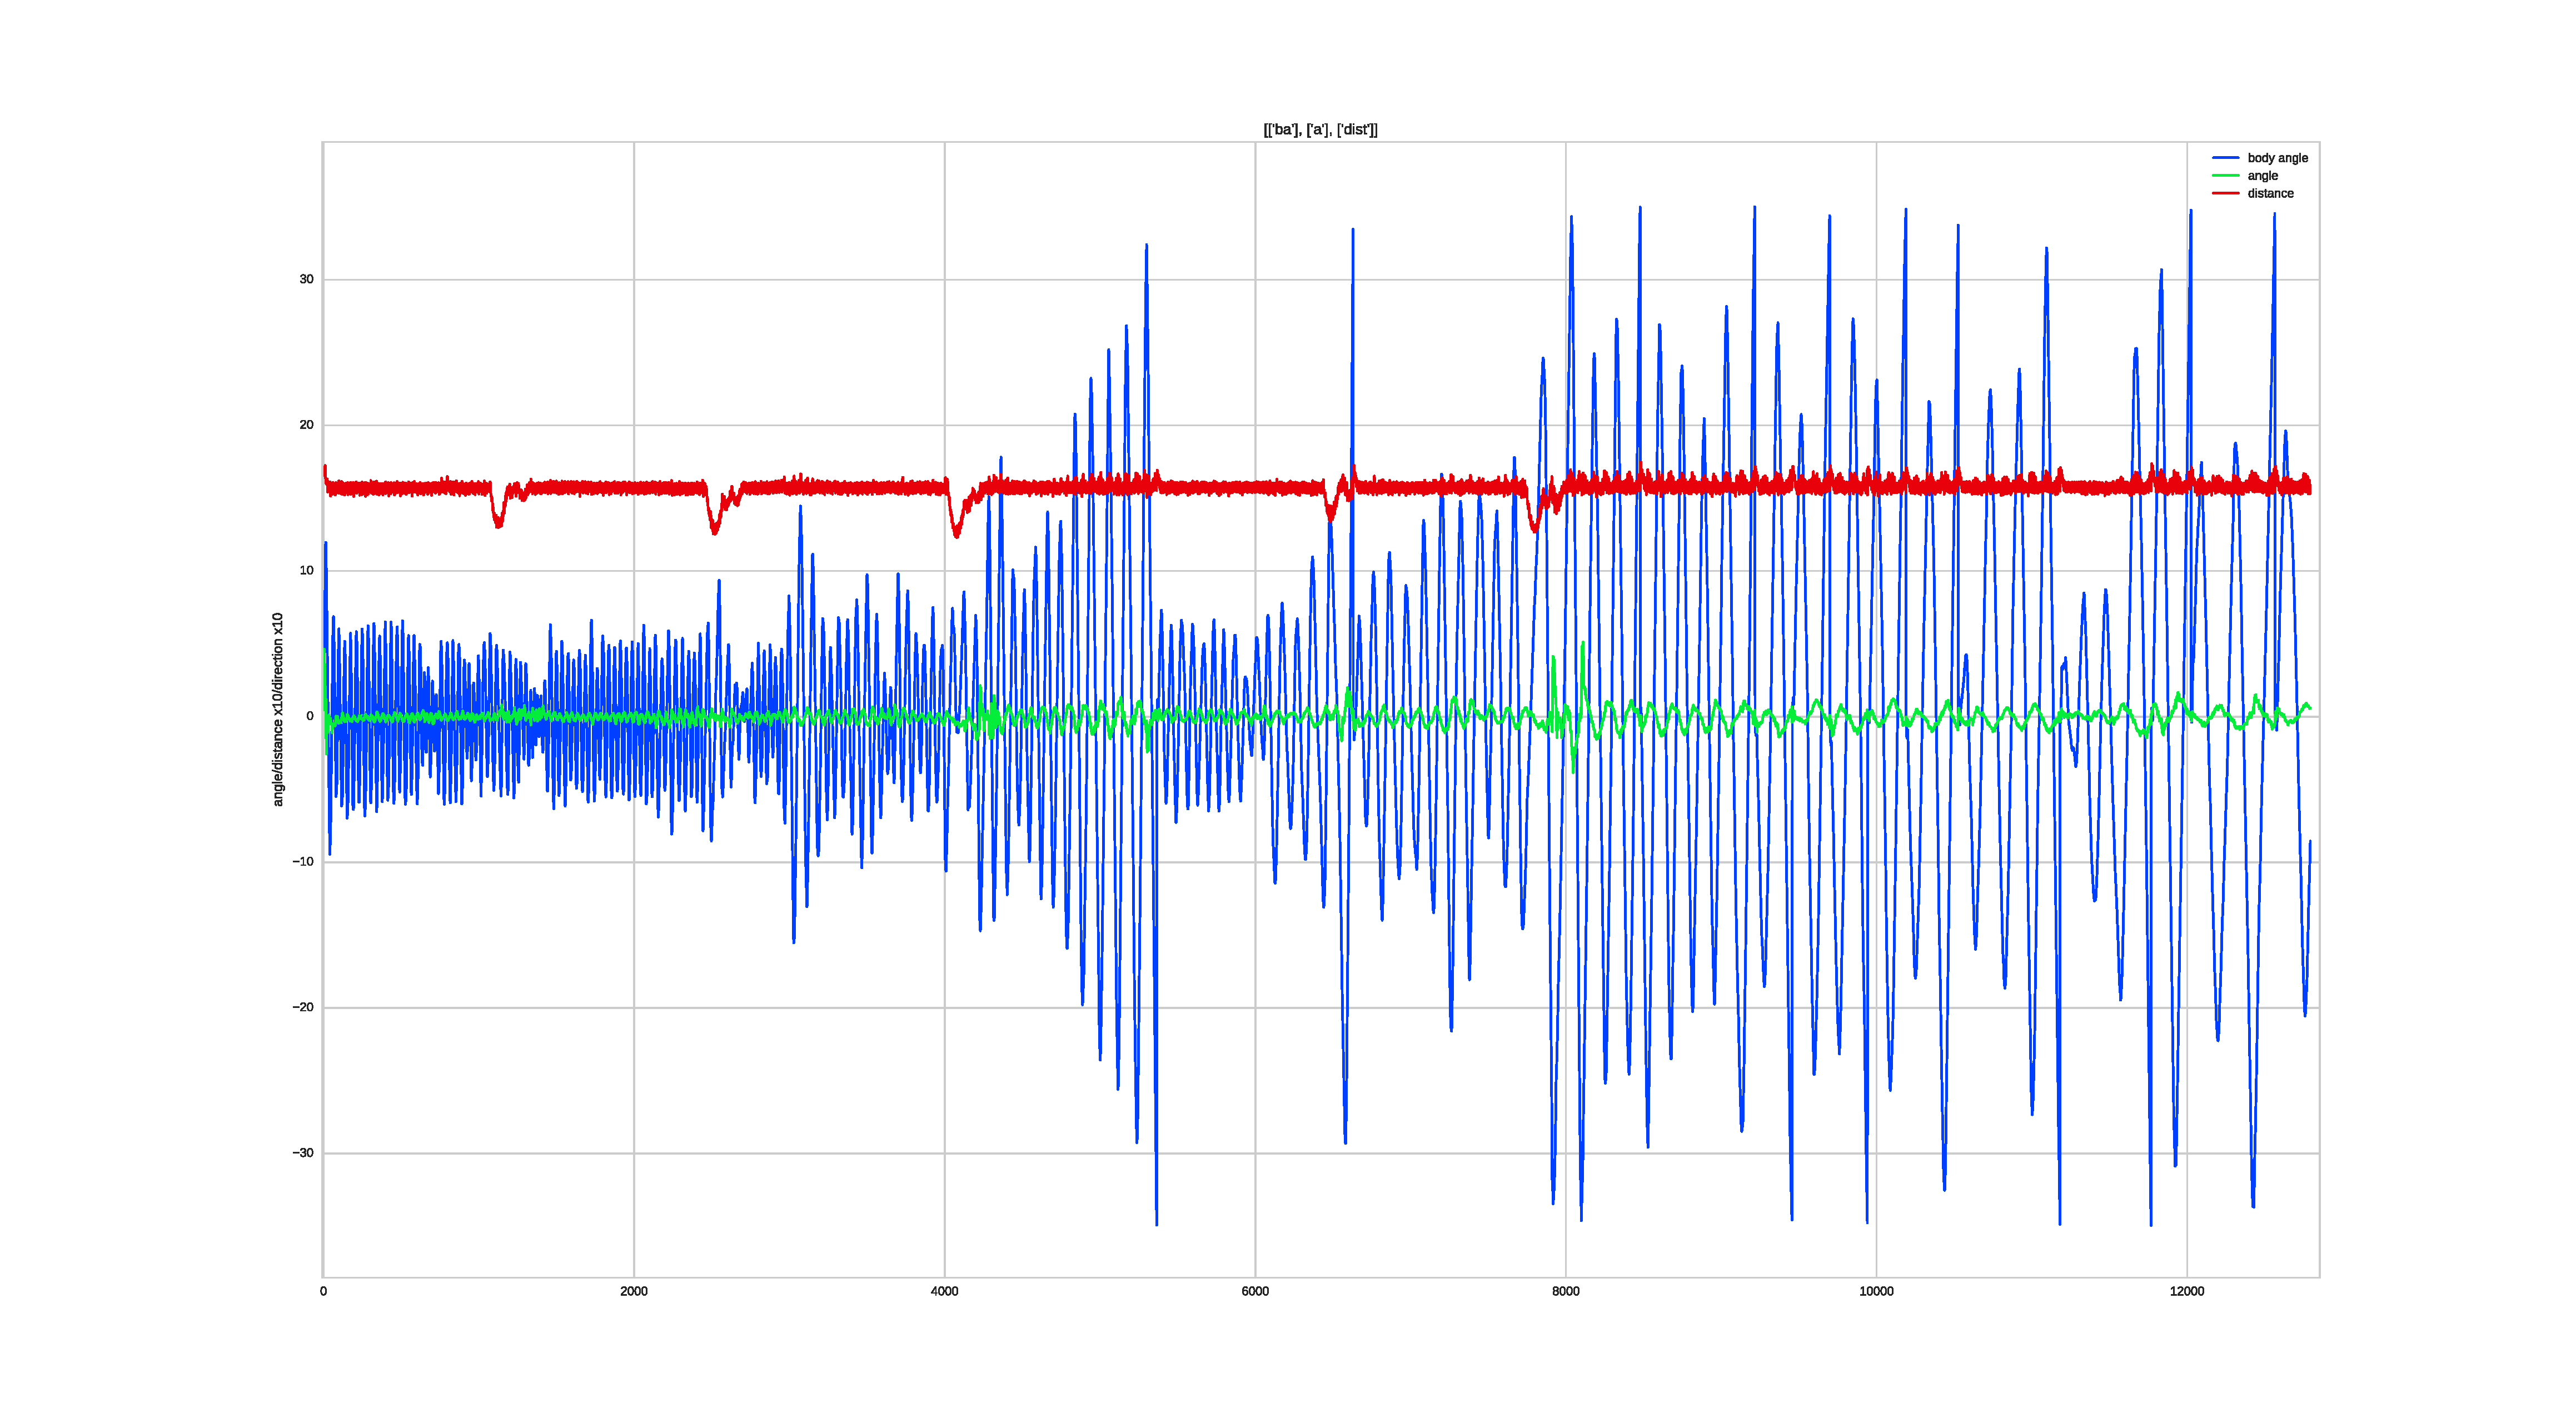
\includegraphics[width=\textwidth]{figures/plots/perfdvsOnlyB2}
  \caption{ Single Layer Network + Head Control: performance in training }
  \label{fig:perfdvsOnlyB2}
\end{figure}
\begin{figure}[htpb]
  \centering
  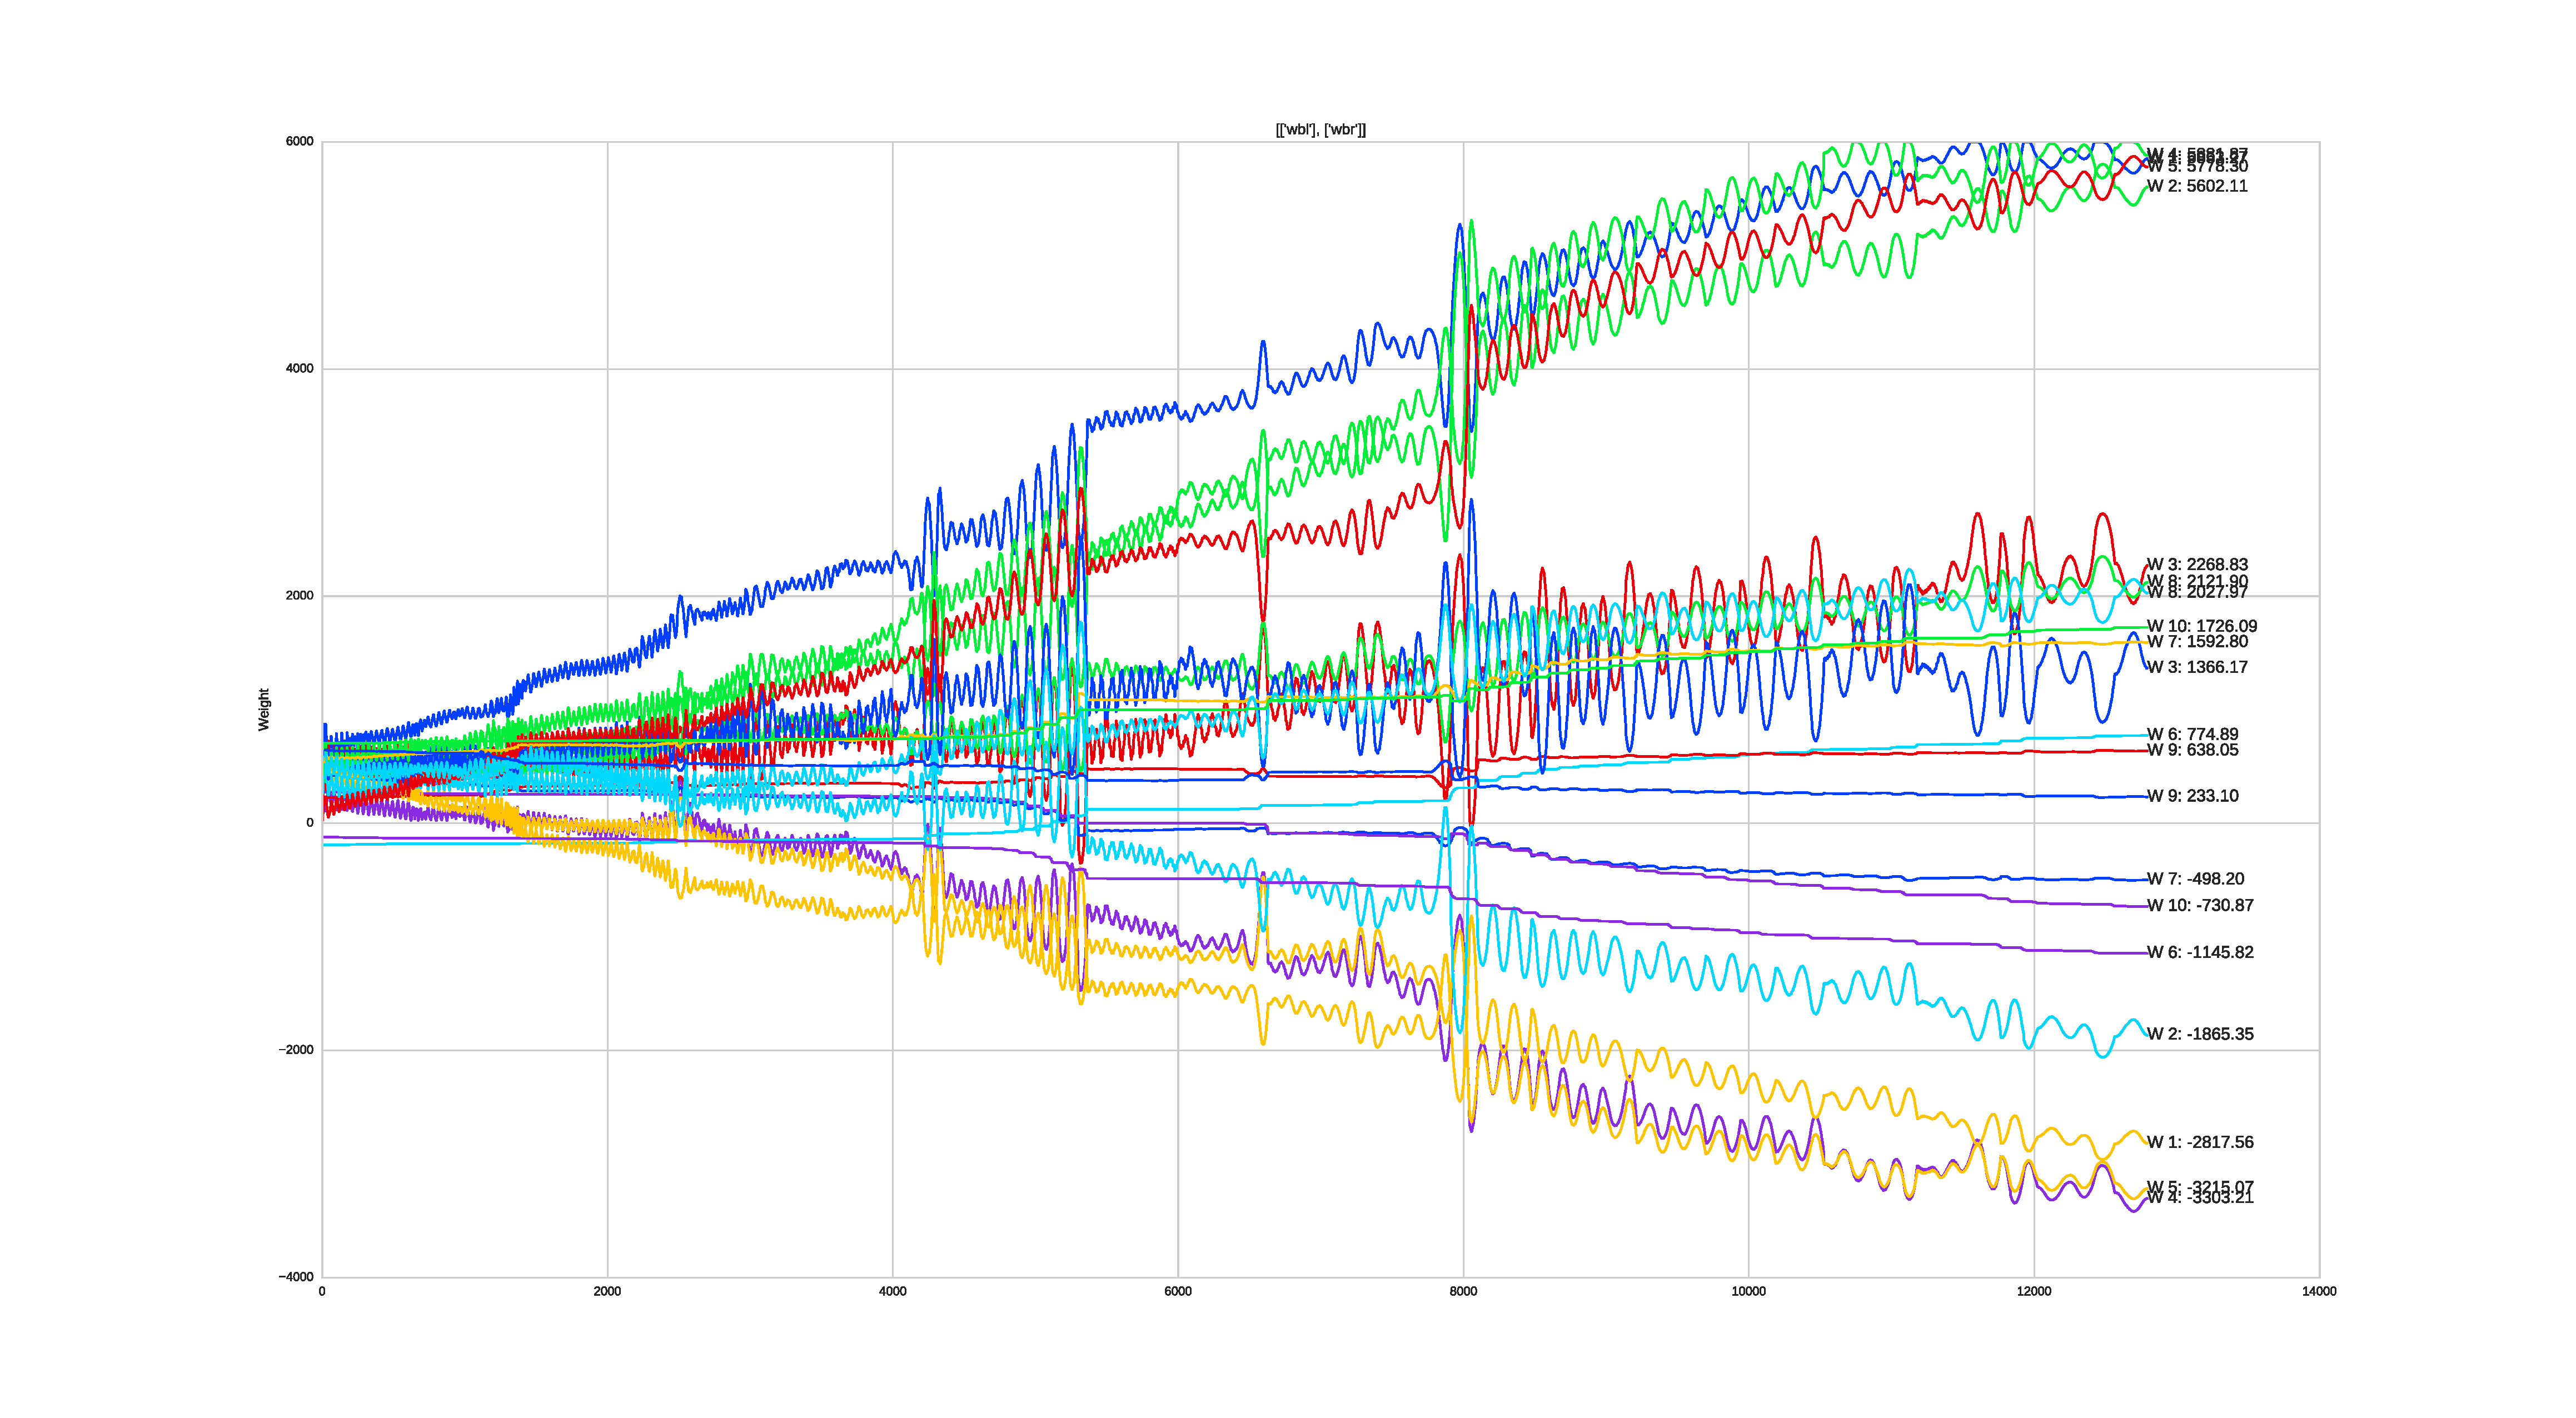
\includegraphics[width=\textwidth]{figures/plots/wblWbrB2Dvs}
  \caption{ Single Layer Network + Head Control: Plot of the weights }
  \label{fig:wblWbrB2Dvs}
\end{figure}
\subsection{Additional Tests}
Having this result additional setups of single layer SNNs with different inputs for the neurons controlling the direction where tested. In the first setup these were connected additionally to the output neurons for head control. In the second setup the input of the body neurons consisted of two neurons each for the first, third and fifth joint of the snake, decoding its angle as described in \autoref{sec:EnOfJoint} and as before the connections to the head output neurons. The other parameters were kept the same.
Both networks showed a similar behavior to the first test case with head control and seem not to be able to solve the task using additional and different inputs. \autoref{fig:baADistB2DvsH} and \autoref{fig:baADistB2JointH} show the mean angles for these two runs and how their performance gets worse over time.

\begin{figure}[htpb]
  \centering
  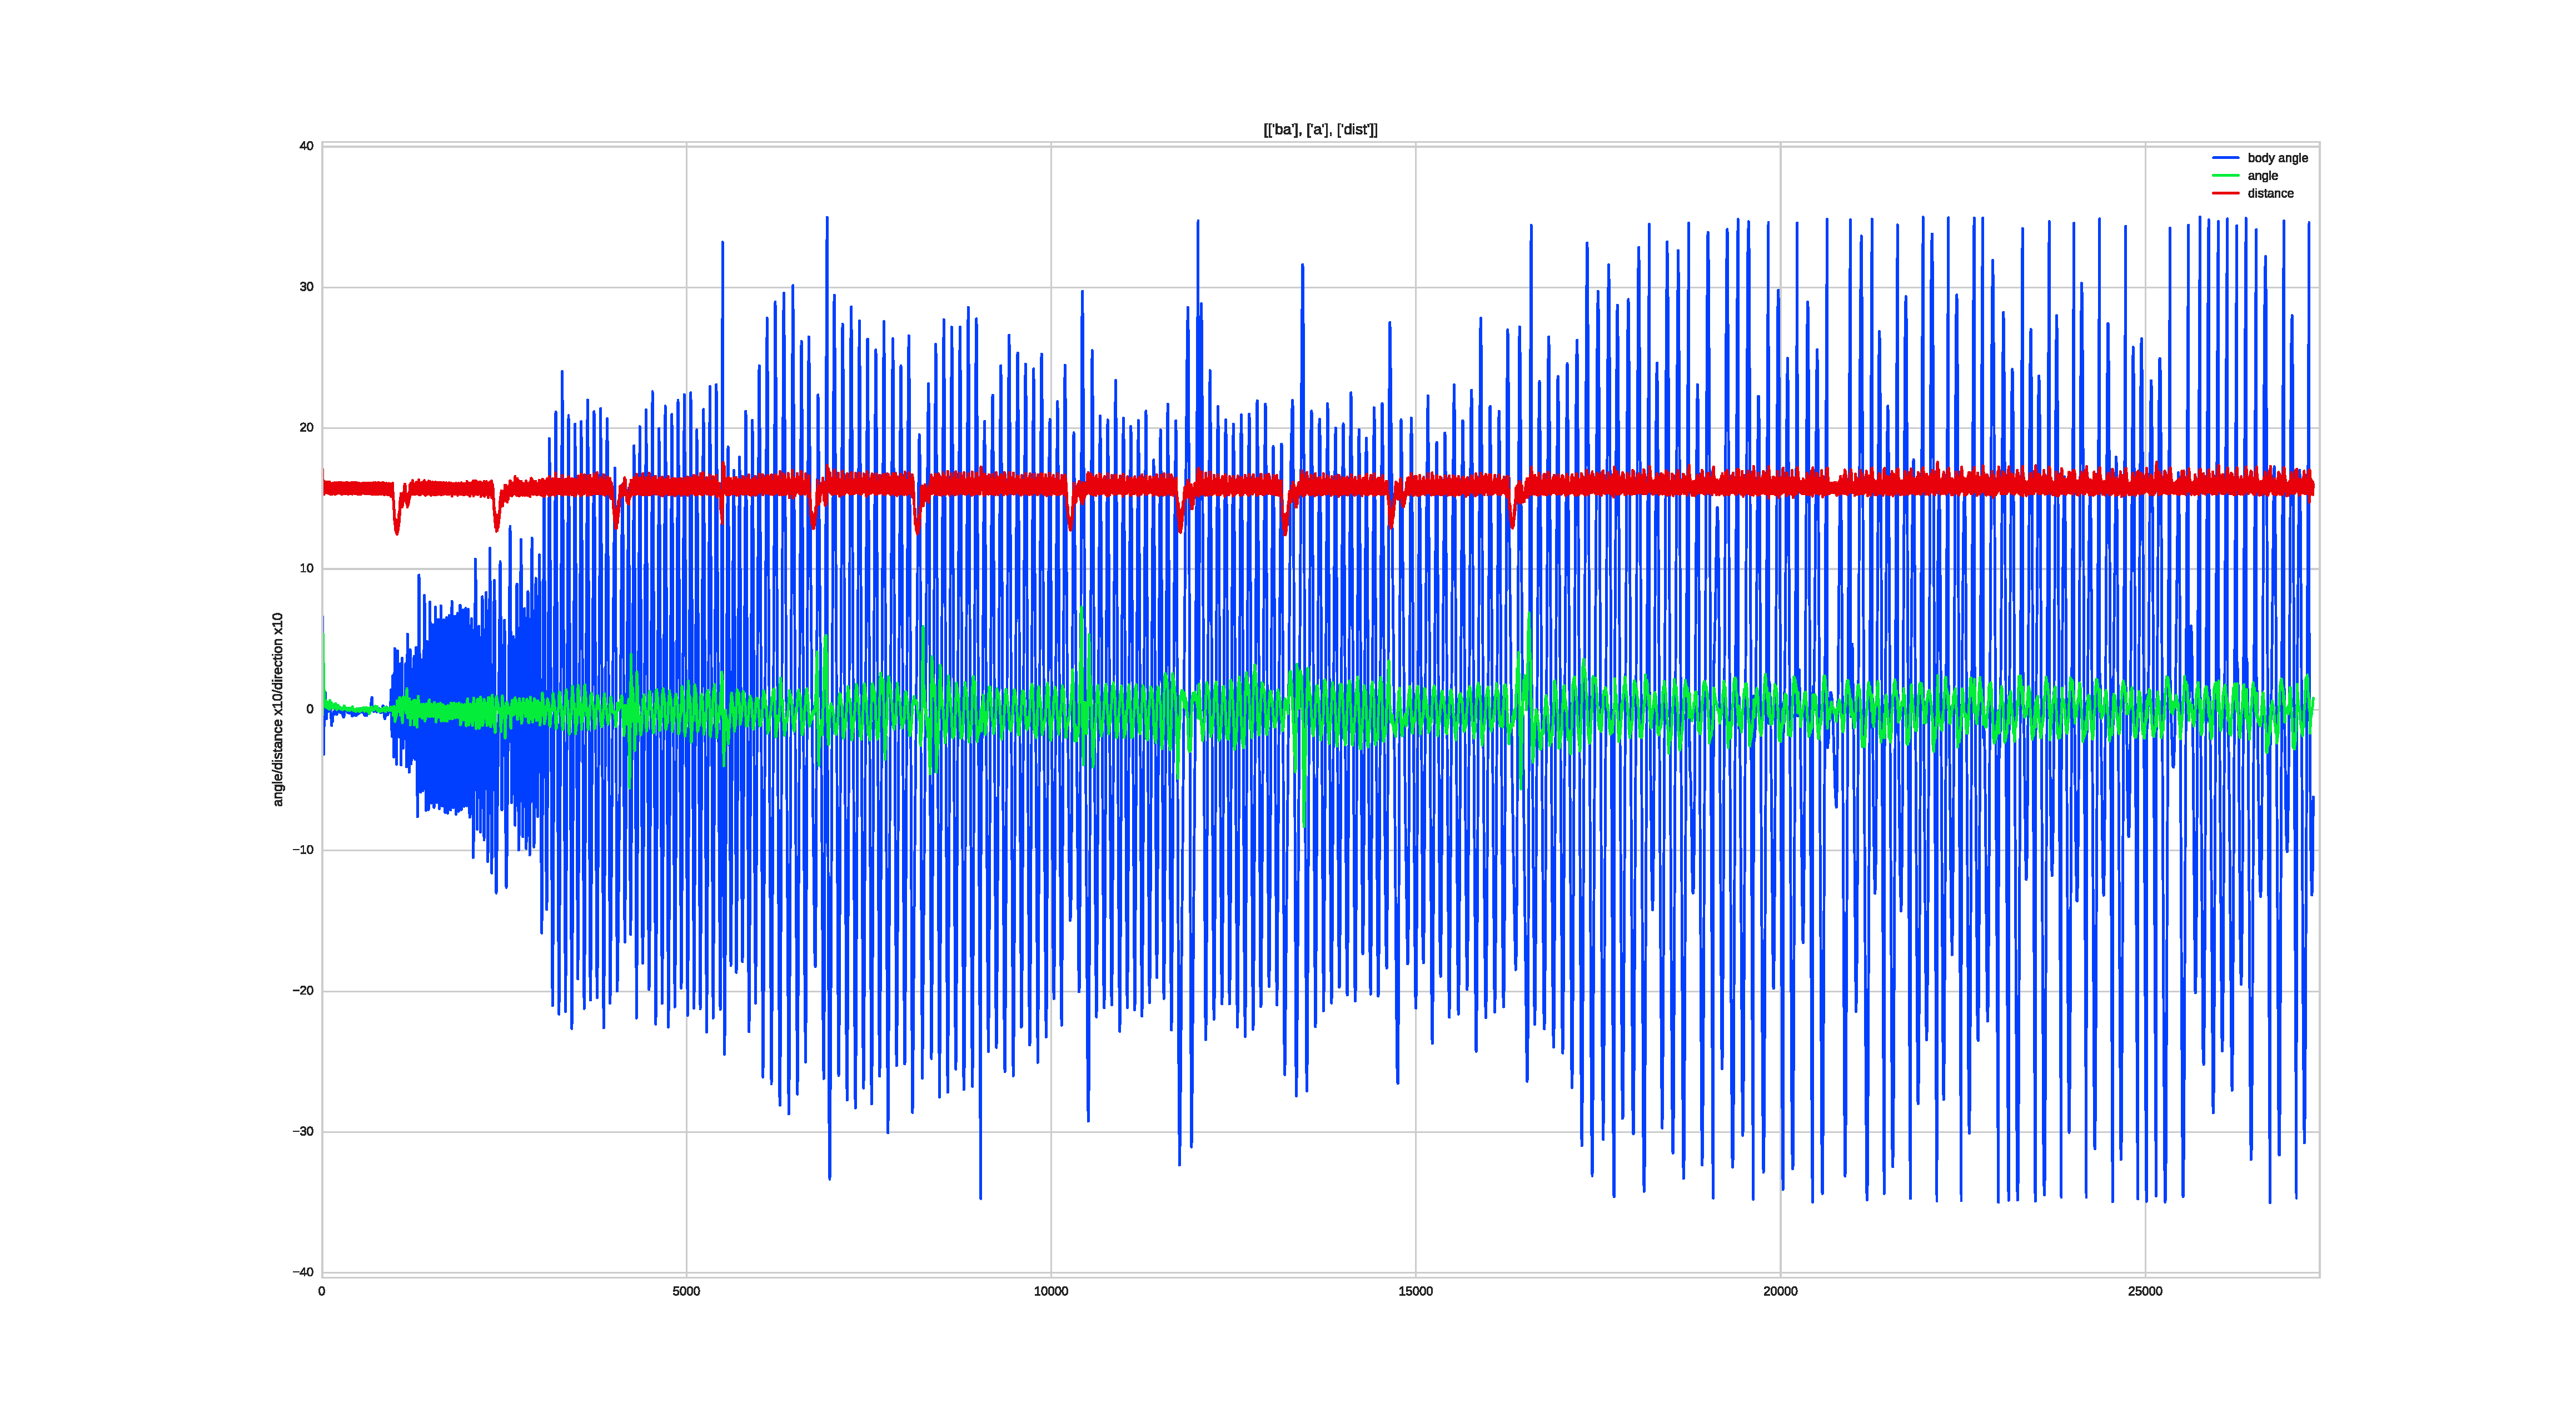
\includegraphics[width=\textwidth]{figures/plots/baADistB2JointH}
  \caption{ Performance of SNN with Joint Angles and Head output as input (training) }
  \label{fig:baADistB2JointH}
\end{figure}
\begin{figure}[htpb]
  \centering
  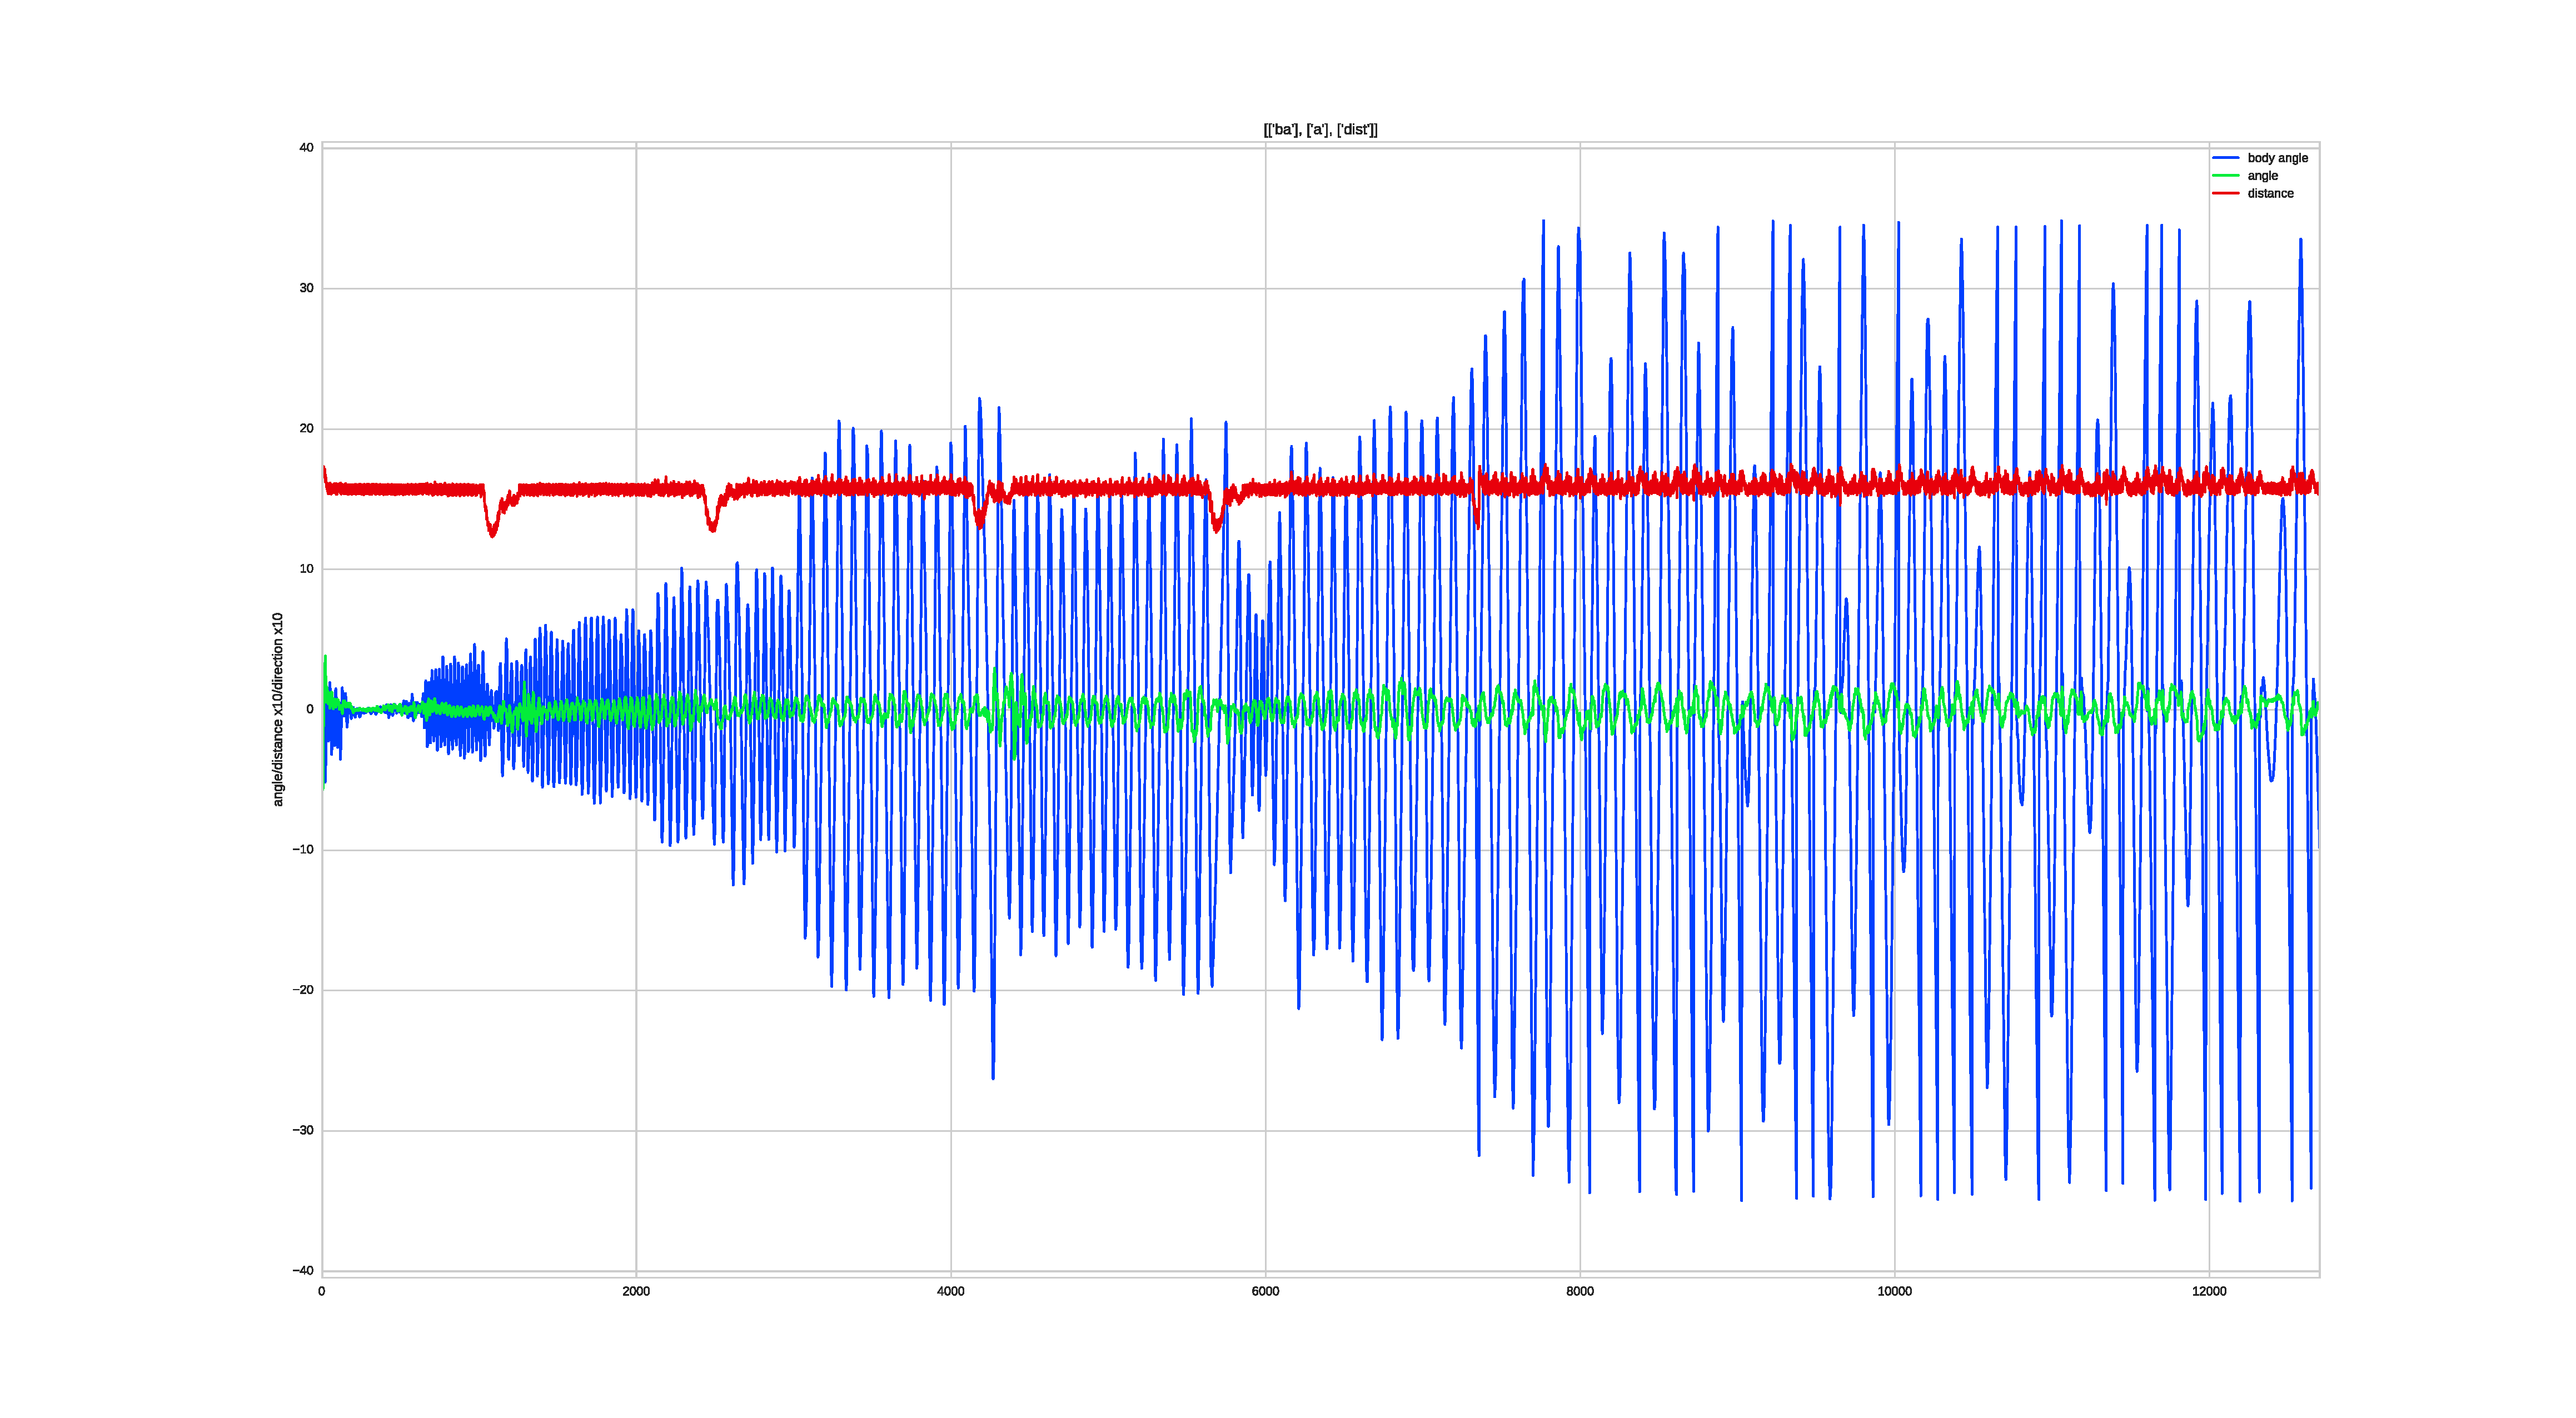
\includegraphics[width=\textwidth]{figures/plots/baADistB2DvsH}
  \caption{ Performance of SNN with DVS and Head output as input (training)  }
  \label{fig:baADistB2DvsH}
\end{figure}

\section{Multi layer Networks}
Previous experiments suggest that a single layered network lacks complexity to solve this task and thus the next experiments will use a second, hidden layer. As the control of the head worked good in the last three examples the head output neurons get still directly connected to only the dvs layer and rewarded as before. Similar to the last experiment six neurons encoding the joint angles and the two output neurons of the head control are used for the input of the hidden layer. The idea behind this is that the output of the head neurons should in some degree encode the information from the DVS input and the angles of the joints but especially the angle of the head joint describe the state of the body. The first, third and fifth joint are chosen as these are the first joints responsible for horizontal movement in the slithering gate of the snake.

\subsection{Single Hidden Layer}
In the first multilayered setup the hidden layer consists of eight neurons, which is the same amount as it has inputs, and the two layers are connected in an ‘all-to-all’ fashion. The parameters for the hidden neurons are shown in \autoref{tab:M1hiddenN} with the main difference in their capacity being higher than previews neurons. For synapses between the input and the hidden layer the parameters shown in \autoref{tab:M1SynH} are used. $tau_{c}$ is set to a higher value compared to previews synapses, with the effect that the eligibility is accumulated over a larger time span and thus the synapse remembers its responsibility for triggering the neuron it connects to for a longer time. This would result in a higher absolute value for the eligibility which would lead to drastic changes of the weights; to counteract this the values for the positive and the negative STDP learning window are scaled down by the same factor $tau_{c}$ is scaled up. For the assignment of the reward to each hidden neuron the backpropagation method described in \autoref{sec:rewardAss} is used and the reward is calculated by \autoref{eq:rewardPSimp}. The parameters used for the connections from the hidden layer to the output for the body are shown in \autoref{tab:M1SynOb}, the topologie of the network is displayed in \autoref{fig:M1netTop}.

\begin{figure}[htpb]
  \centering
  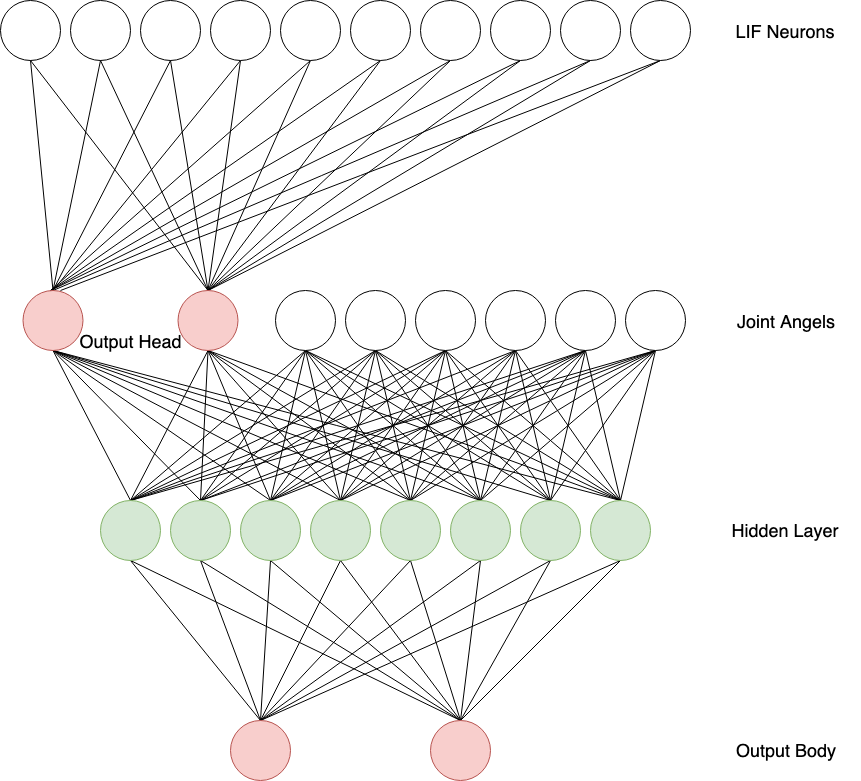
\includegraphics[width=\textwidth]{figures/plots/M1NetworkTop}
  \caption{ Sketch of Network Topology for the Network with one hidden layer  }
  \label{fig:M1netTop}
\end{figure}

% \def\layersep{2.5cm}
% \begin{tikzpicture}[shorten >=1pt,->,draw=black!50, node distance=\layersep]
%   \tikzstyle{every pin edge}=[<-,shorten <=1pt]
%   \tikzstyle{neuron}=[circle,fill=black!25,minimum size=17pt,inner sep=0pt]
%   \tikzstyle{input neuron}=[neuron, fill=green!50];
%   \tikzstyle{output neuron}=[neuron, fill=red!50];
%   \tikzstyle{hidden neuron}=[neuron, fill=blue!50];
%   \tikzstyle{annot} = [text width=4em, text centered]

%   % Draw the input layer nodes
%   \foreach \name / \y in {1,...,16}
%   % This is the same as writing \foreach \name / \y in {1/1,2/2,3/3,4/4}
%       \node[input neuron, pin=left:Input \#\y] (I-\name) at (0,-\y) {};

%   % Draw the hidden layer nodes
%   \foreach \name / \y in {1,...,8}
%       \path[yshift=0.5cm]
%           node[hidden neuron] (H-\name) at (\layersep,-\y cm) {};

%   % Draw the output layer node
%   \foreach \name / \y in {1,...,4}
%     \node[output neuron,pin={[pin edge={->}]right:Output \#\y}, right of=H-3] (\layersep*2,-\y) {};

%   % Connect every node in the input layer with every node in the
%   % hidden layer.
%   \foreach \source in {1,...,10}
%       \foreach \dest in {1,...,2}
%           \path (I-\source) edge (O-\dest);

%   % Connect every node in the hidden layer with the output layer
%   \foreach \source in {1,...,5}
%       \path (H-\source) edge (O);

%   % Annotate the layers
%   \node[annot,above of=H-1, node distance=1cm] (hl) {Hidden layer};
%   \node[annot,left of=hl] {Input layer};
%   \node[annot,right of=hl] {Output layer};
% \end{tikzpicture}


\begin{table}[htpb]
  \centering
  \caption[Parameters Single Hidden Layer]{Parameters of the hidden synapses for the single hidden layer setup} \label{tab:M1SynH}
  \begin{tabular}{|c| c |l|}
      \toprule
      Parameter  & Value & Description \\
      \midrule
      $W_{max}$ & 6000   & Maximum weight of synapse\\   
      $W_{min}$ & -6000  & Minimum weight of synapse\\   
      $A_{+}$   & 0.002    & Constant scaling strength of potentiation\\   
      $A_{-}$   & -0.001   & Constant scaling strength of depression \\   
      $\tau_c$  & 10000.0   & Time constant of eligibility trace \\  
      $\tau_n$  & 20.0   & Time constant of reward signal  \\   
      $b$       & 0.0    & Baseline neuromodulator concentration \\    
      \bottomrule
  \end{tabular}
\end{table}
  
  \begin{table}[htpb]
  \centering
  \caption[Parameters 2.Setup]{Parameters of hidden Neurons for the single hidden layer setup} \label{tab:M1hiddenN}
    \begin{tabular}{|c| c |l|}
      \toprule
      Parameter & Value & Description \\
      \midrule
      $c_m$   & 100.0  & Capacity of the membrane \\
      $tau_{m}$    & 50.0  & Membrane time constant \\
      $tau_{refrac}$   & 1.  & Duration of refractory period\\
      $v_{thresh}$   & -50.0  & Spike initiation threshold \\
      $v_{reset}$    & -65.0  &  Reset value for $V_m$ after a spike \\
      $v_{rest}$ & -65.0 & Resting voltage for $V_m$ \\
      \bottomrule
    \end{tabular}
  \end{table}

  \begin{table}[htpb]
  \centering
  \caption[Parameters Single Hidden Layer]{Parameters of the body output synapses for the single hidden layer setup} \label{tab:M1SynOb}
    \begin{tabular}{|c| c |l|}
        \toprule
        Parameter  & Value & Description \\
        \midrule
        $W_{max}$ & 6000   & Maximum weight of synapse\\   
        $W_{min}$ & -6000  & Minimum weight of synapse\\   
        $A_{+}$   & 0.2    & Constant scaling strength of potentiation\\   
        $A_{-}$   & -0.1   & Constant scaling strength of depression \\   
        $\tau_c$  & 100.0   & Time constant of eligibility trace \\  
        $\tau_n$  & 20.0   & Time constant of reward signal  \\   
        $b$       & 0.0    & Baseline neuromodulator concentration \\    
        \bottomrule
    \end{tabular}
  \end{table}
For this setup the learning phase was much longer compared to the single layer network. At the time the weights for the first setup stabilised the weights in this simulation still were under a lot of change. This can be seen by comparing the graph of the weights for the output layer in \autoref{fig:WBase1}, with \autoref{fig:M1Wb} which shows the weights for this setup.
\begin{figure}[htpb]
  \centering
  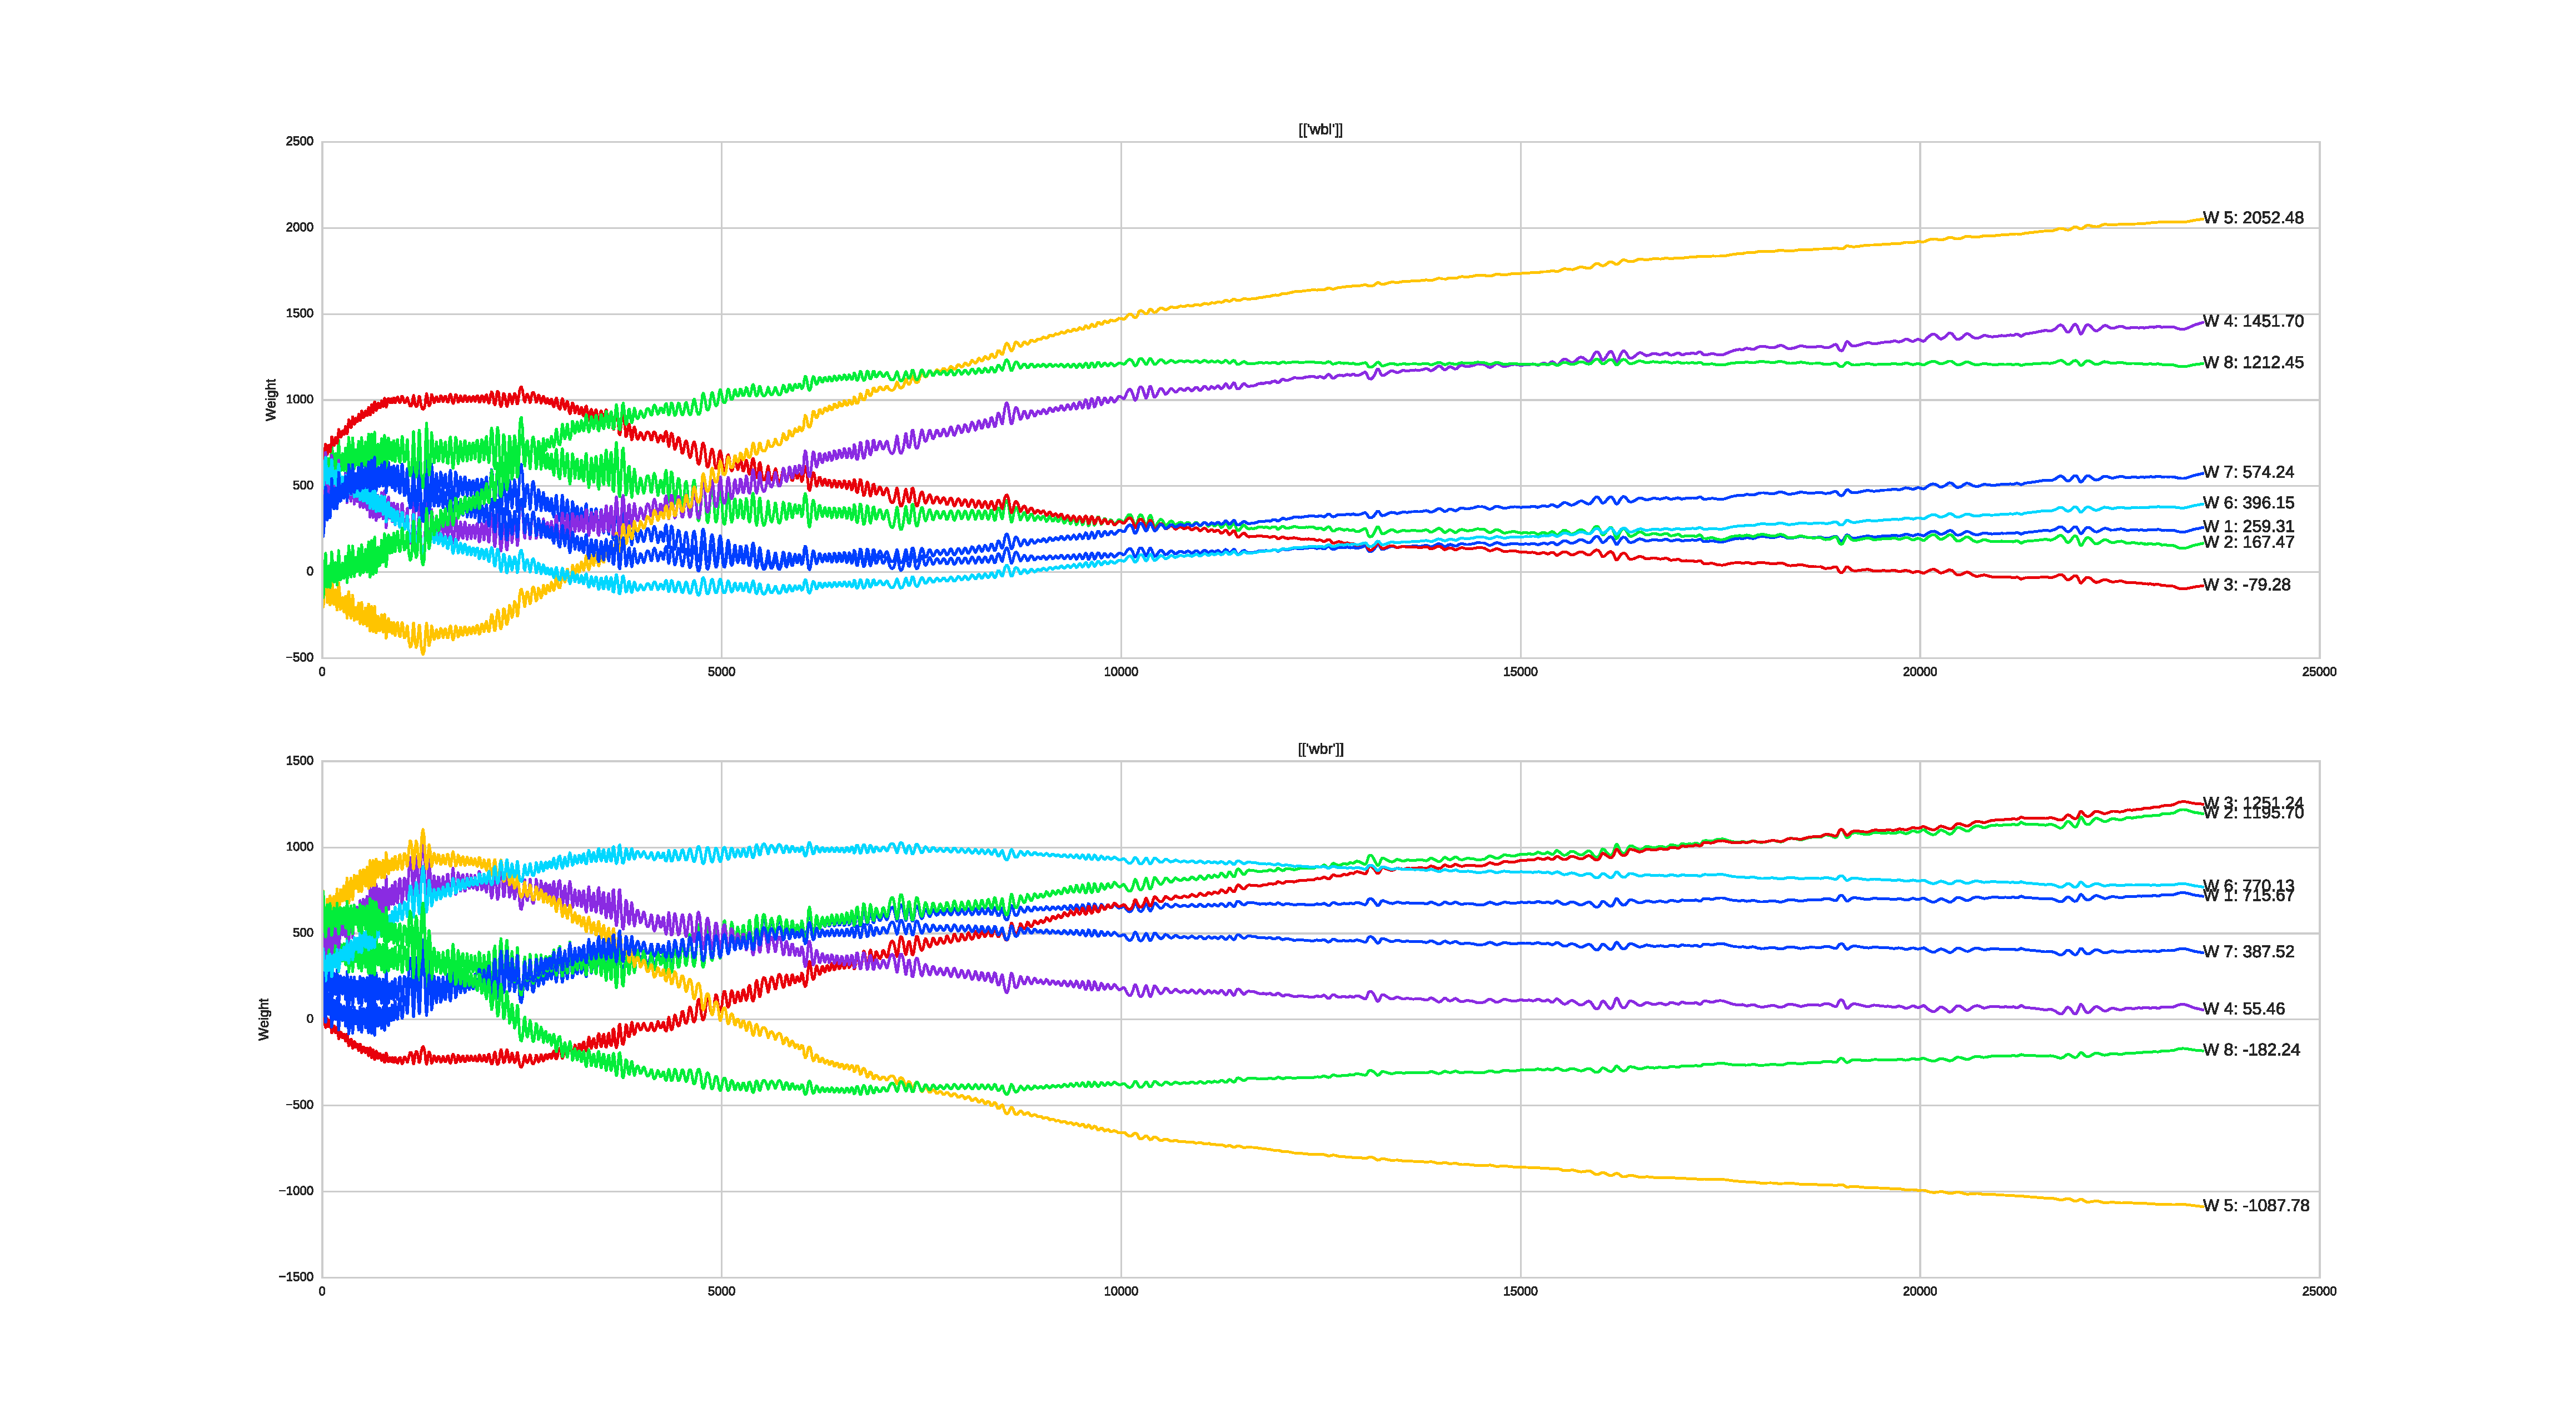
\includegraphics[width=\textwidth]{figures/plots/M1Wb}
  \caption{ Weights connecting the body output of SNN with one hidden Layer (training)  }
  \label{fig:M1Wb}
\end{figure}
While the changes get less over time the network remains able to solve the task with a very good performance of the head and a good result for the mean body angle with peaks of around $25$ degrees towards the end of the training. \autoref{fig:M1baADist} shows the plot of the mean angles as well as the distance to the target for this setup.
\begin{figure}[htpb]
  \centering
  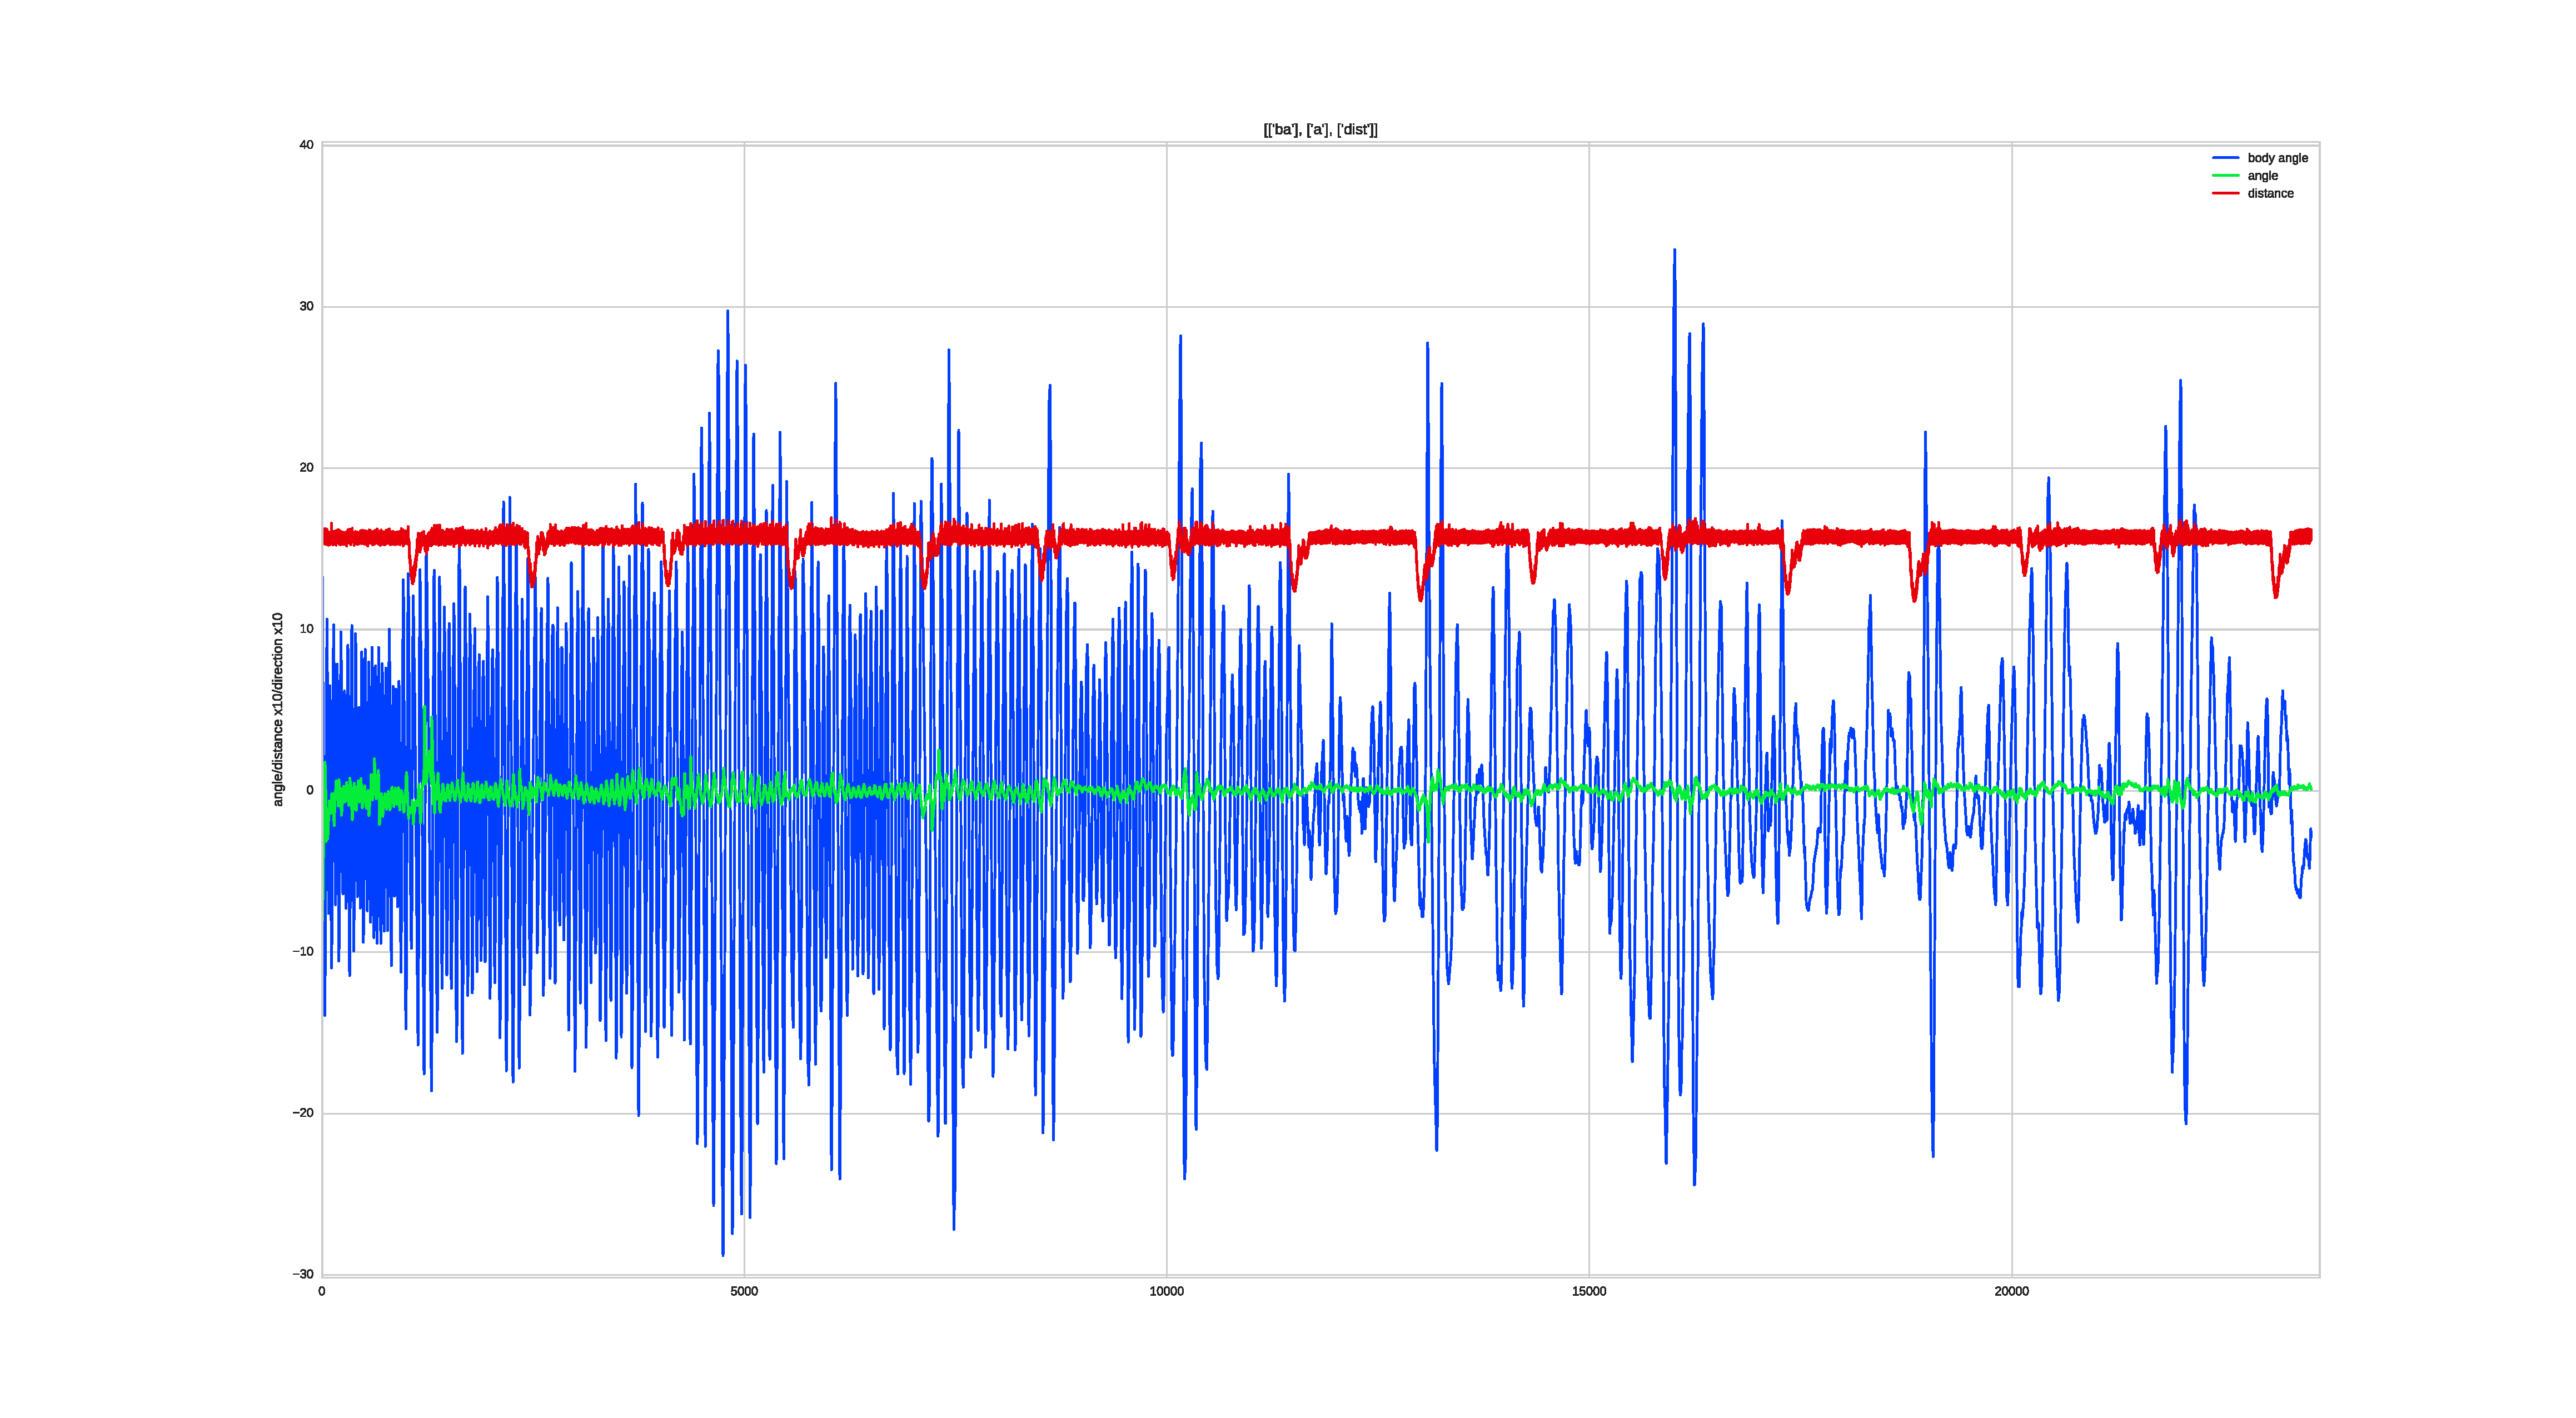
\includegraphics[width=\textwidth]{figures/plots/M1baADist}
  \caption{ Performance of SNN with one hidden Layer (training)  }
  \label{fig:M1baADist}
\end{figure}
\subsection{Split Hidden Layer}
The last network trained is similar to the previous network in all parameters, the only difference lies in the topologie of the network. As shown in \autoref{fig:M2netTop} the hidden layer is split in two pairs of four neurons each and all outgoing connections from a pair go to only one neuron in the output layer. \autoref{eq:rewardPSimp} simplifies for this setup to

\begin{figure}[htpb]
  \centering
  \includegraphics[width=\textwidth]{figures/plots/M2netTop}
  \caption{ Sketch of Network Topology for the Network with split hidden layer  }
  \label{fig:M2netTop}
\end{figure}

\begin{equation}
r_h = r * \frac{w_r} {|w_r|)}
\end{equation}
for the hidden layer connected to the right output and
\begin{equation}
r_h = - r * \frac{w_l} {|w_l|)}
\end{equation}
for the hidden layer connected to the left output. This simplification is the result of hidden neurons influencing only one other neuron. In this equitations $w_l$/$w_r$ are the weights of the connection from a neuron in left/right hidden layer to its output and $r$ is the reward for the output, calculated as before.
Training the network took about as long as for the other multilayered network and the overall performance is comparable but this version had spikes in the mean body angle of around $32$ degrees. The plot of the mean angles for this training is shown in \autoref{fig:baADistMS}.
\begin{figure}[htpb]
  \centering
  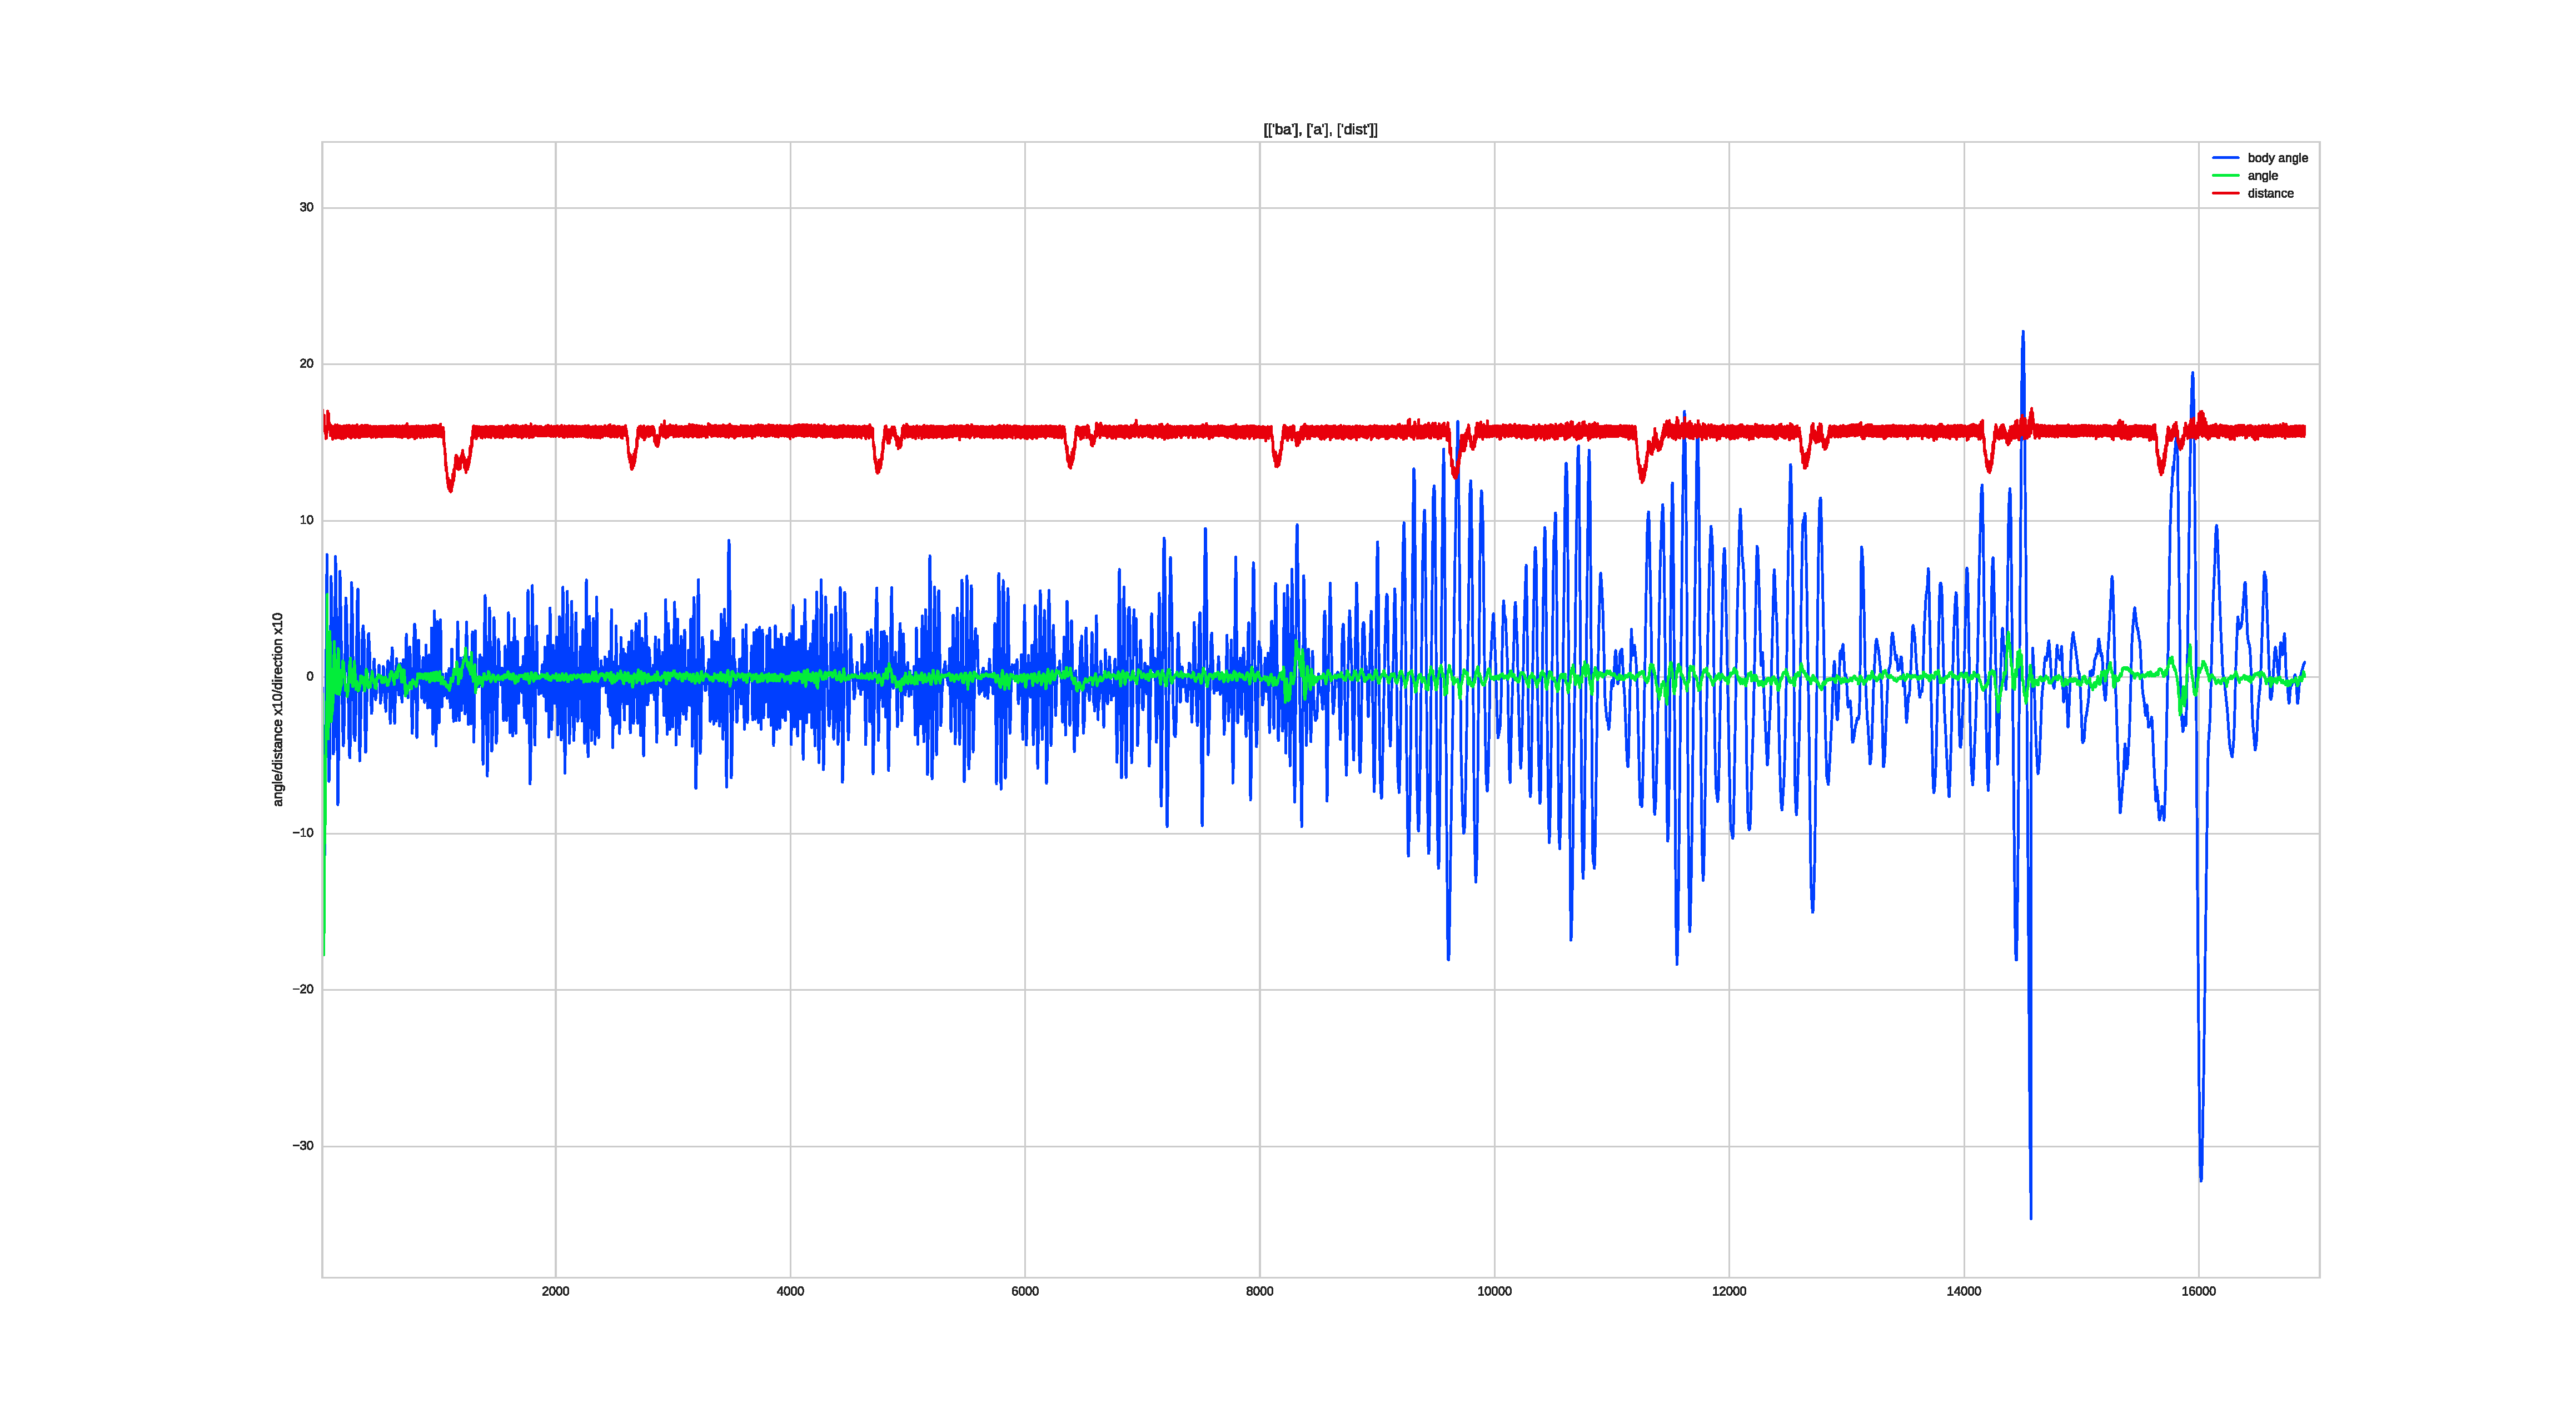
\includegraphics[width=\textwidth]{figures/plots/baADistMS}
  \caption{ Performance of SNN with a split hidden Layer (training)  }
  \label{fig:baADistMS}
\end{figure}

\chapter{Testing}
To test the performance of the trained networks a different path for the target is chosen. The shape of the new path, shown in \autoref{fig:testPath}, has a similar curvature to the training path but a different progression. This way the snake should still be able to finish the test but also faces new situations. 

\section{Test results}
First the basic setup was tested and finished the task two times without any error. In the second run the path was mirrored on the $y$-Axe. As seen in \autoref{fig:B1_A} mean angle to the ball never surpasses an absolute value of $4$ degrees which is quite impressive.
\newline
\begin{figure}[htpb]
  \centering
  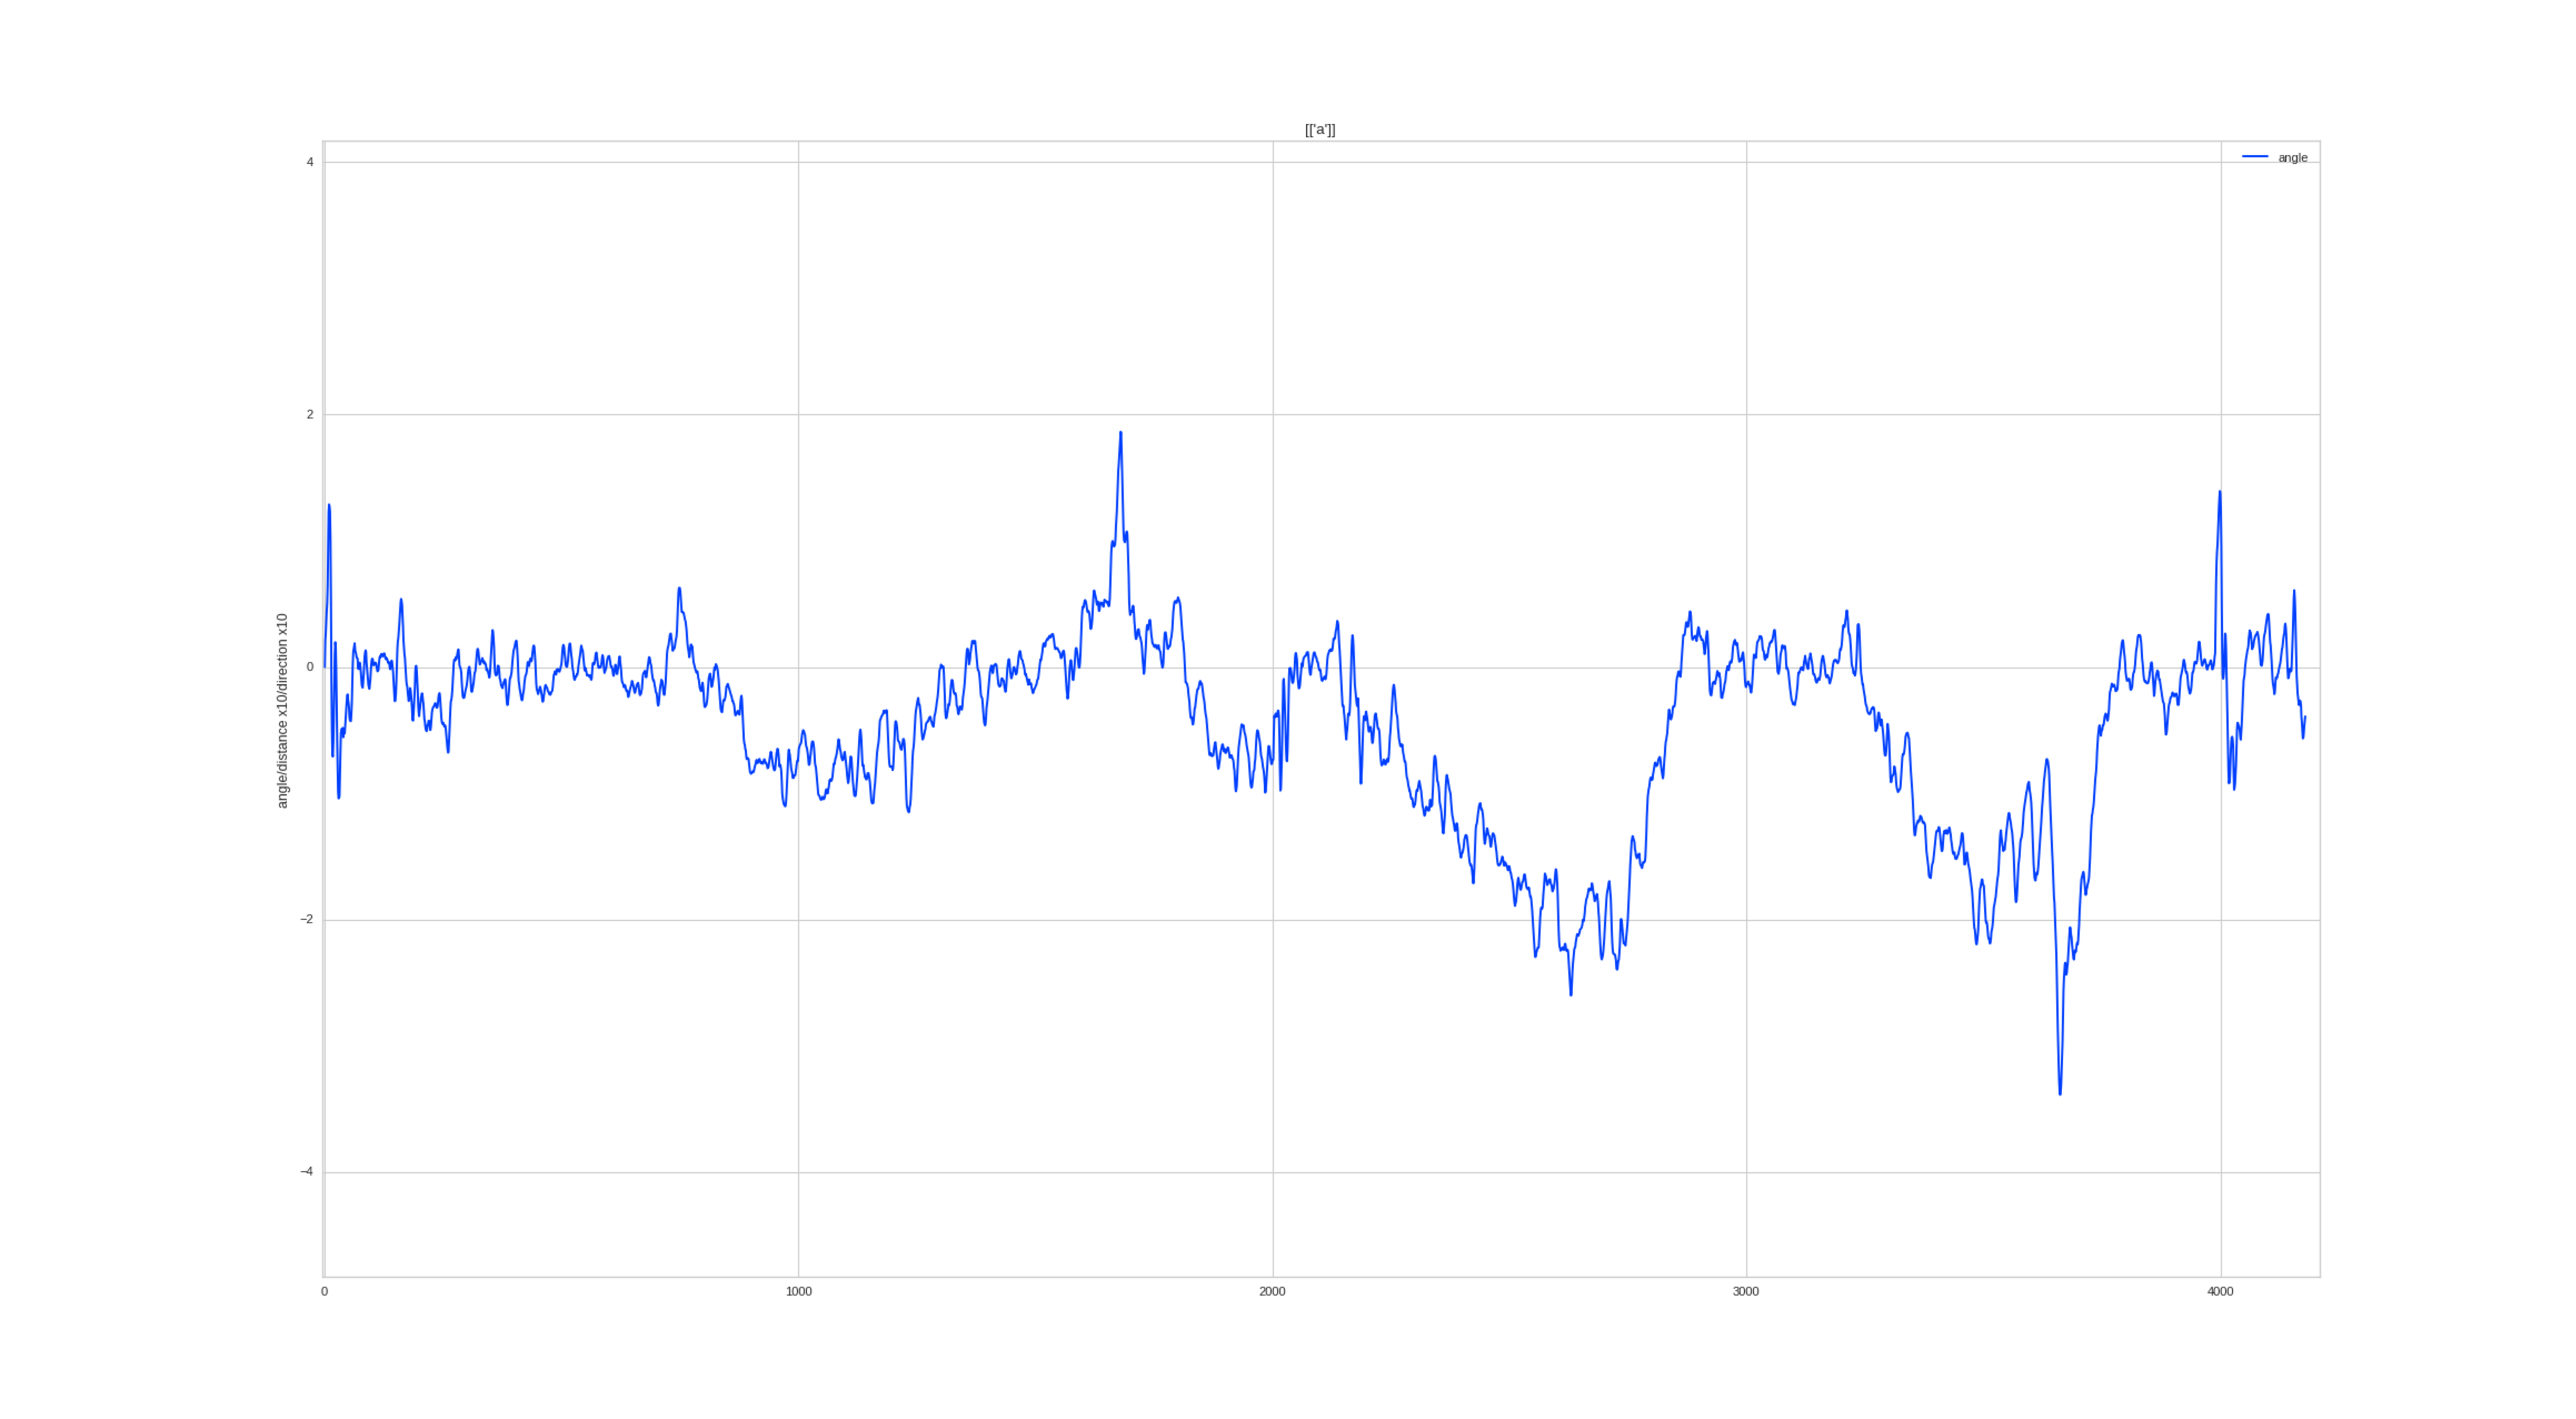
\includegraphics[width=\textwidth]{figures/plots/B1_A}
  \caption{ Performance of the basic network in the test }
  \label{fig:B1_A}
\end{figure}
Next the network with the single hidden layer was tested and even though it seemed as the weights head stabilised at the end of the training simulation, the network was not able to perform at all and never made it to the first turn. \autoref{fig:M1_perf} shows how the network fails as it has a too high affinity to go left.
\begin{figure}[htpb]
  \centering
  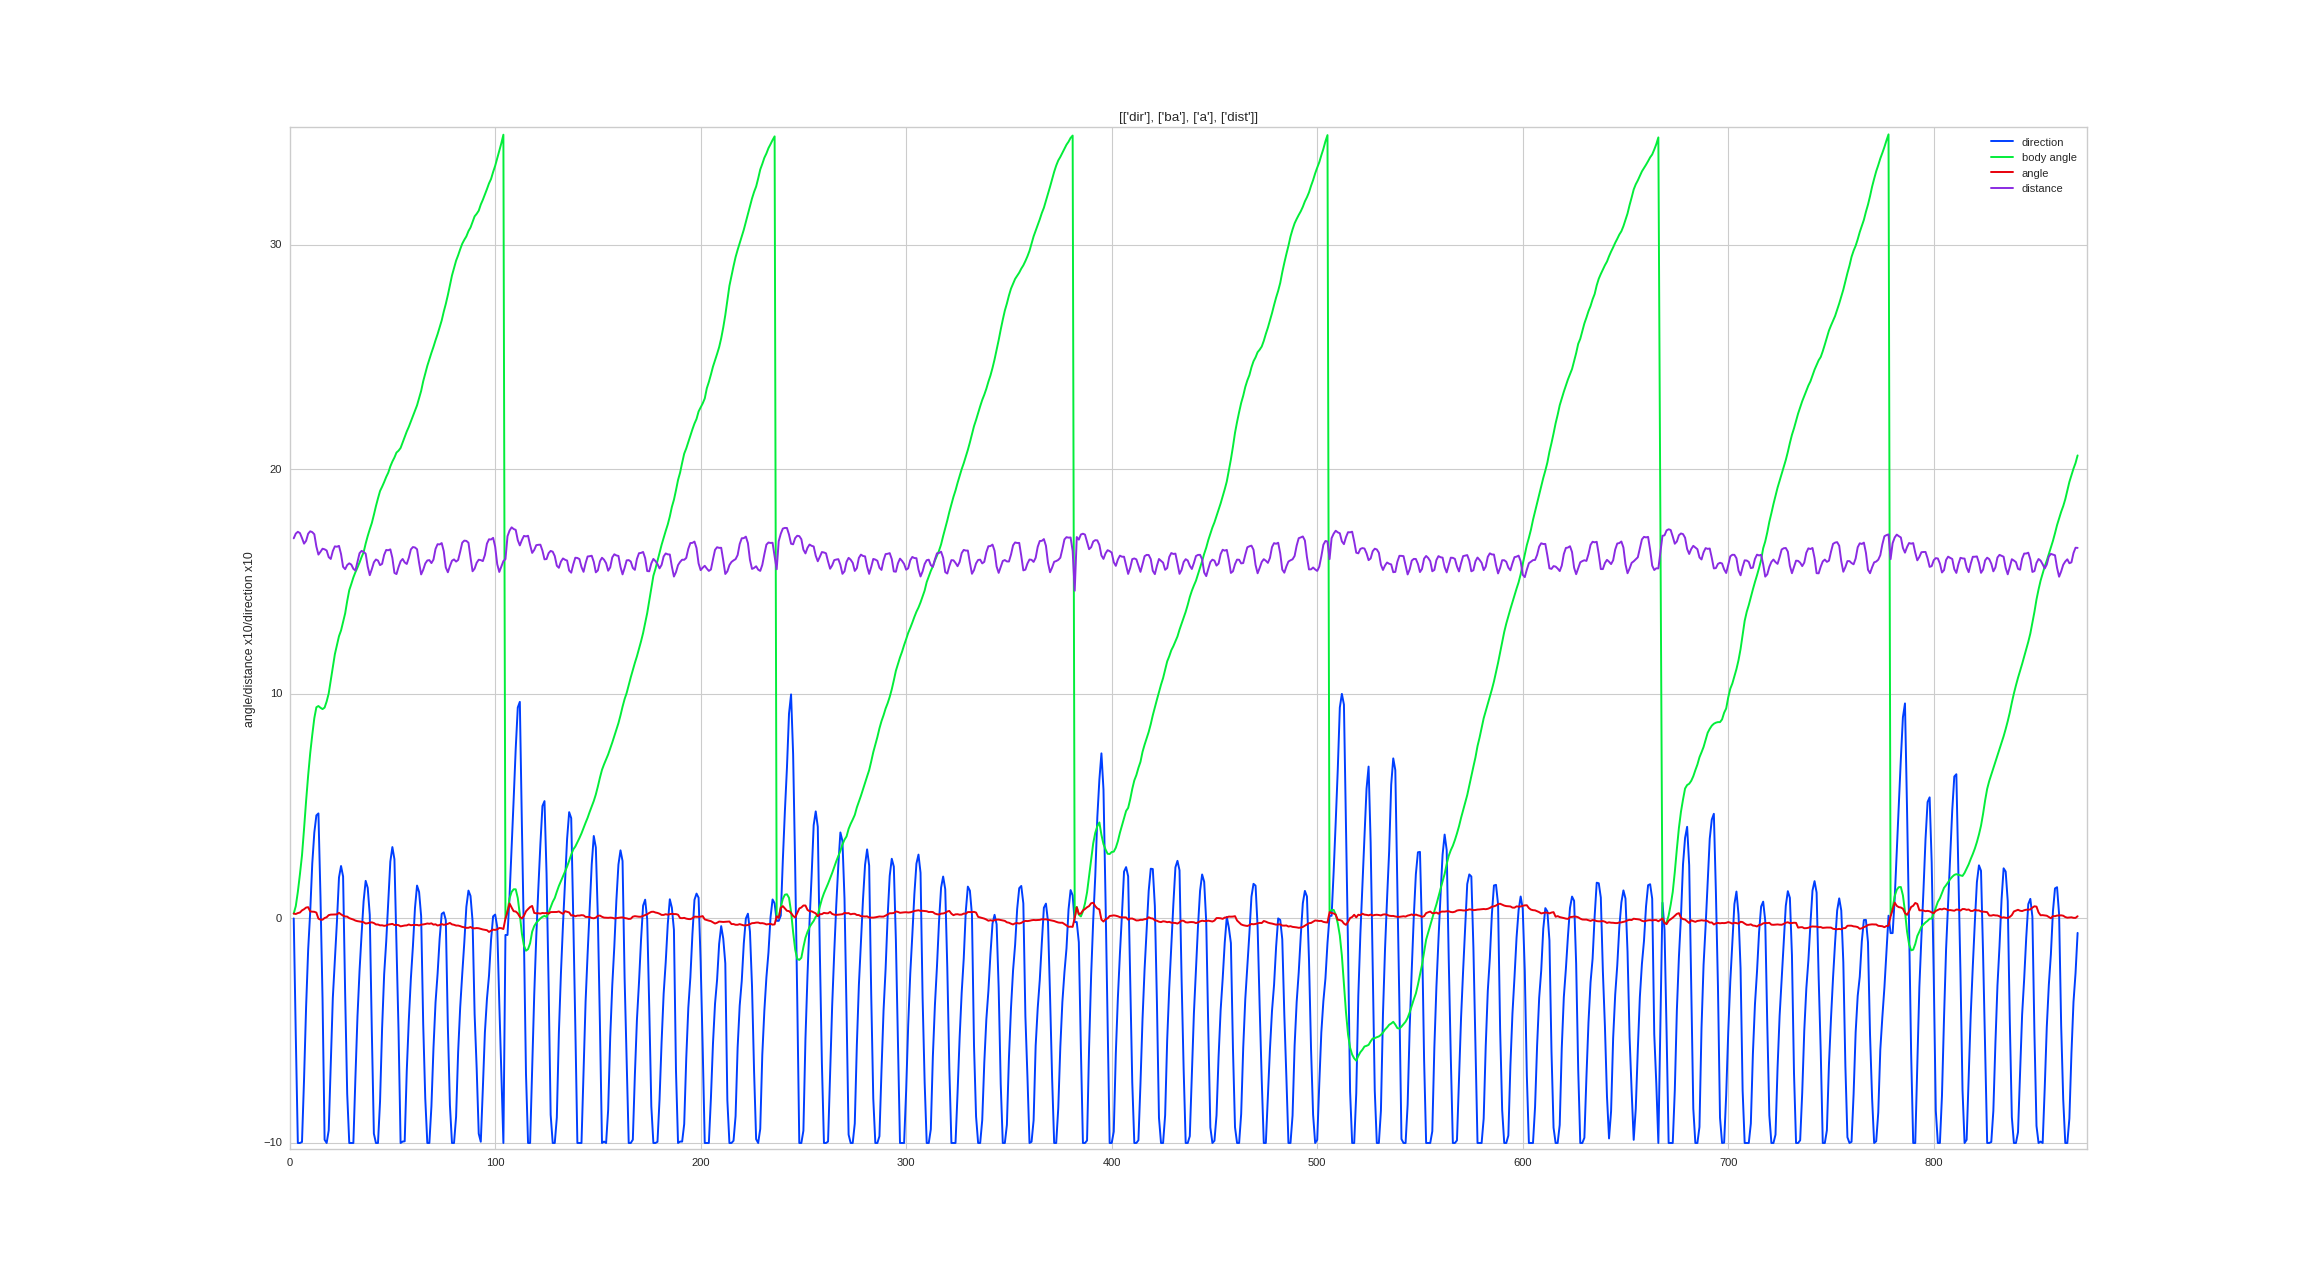
\includegraphics[width=\textwidth]{figures/plots/M1_perf}
  \caption{ Performance of the multilayer network with one hidden layer in the test }
  \label{fig:M1_perf}
\end{figure}
\newline
As last the network with the split hidden layer is tested. It performance well and keeps the mean body angl most time below $5$ degrees while its head angle is moste time lower than $1$ degree, see \autoref{fig:M2-baADist}.
\begin{figure}[htpb]
  \centering
  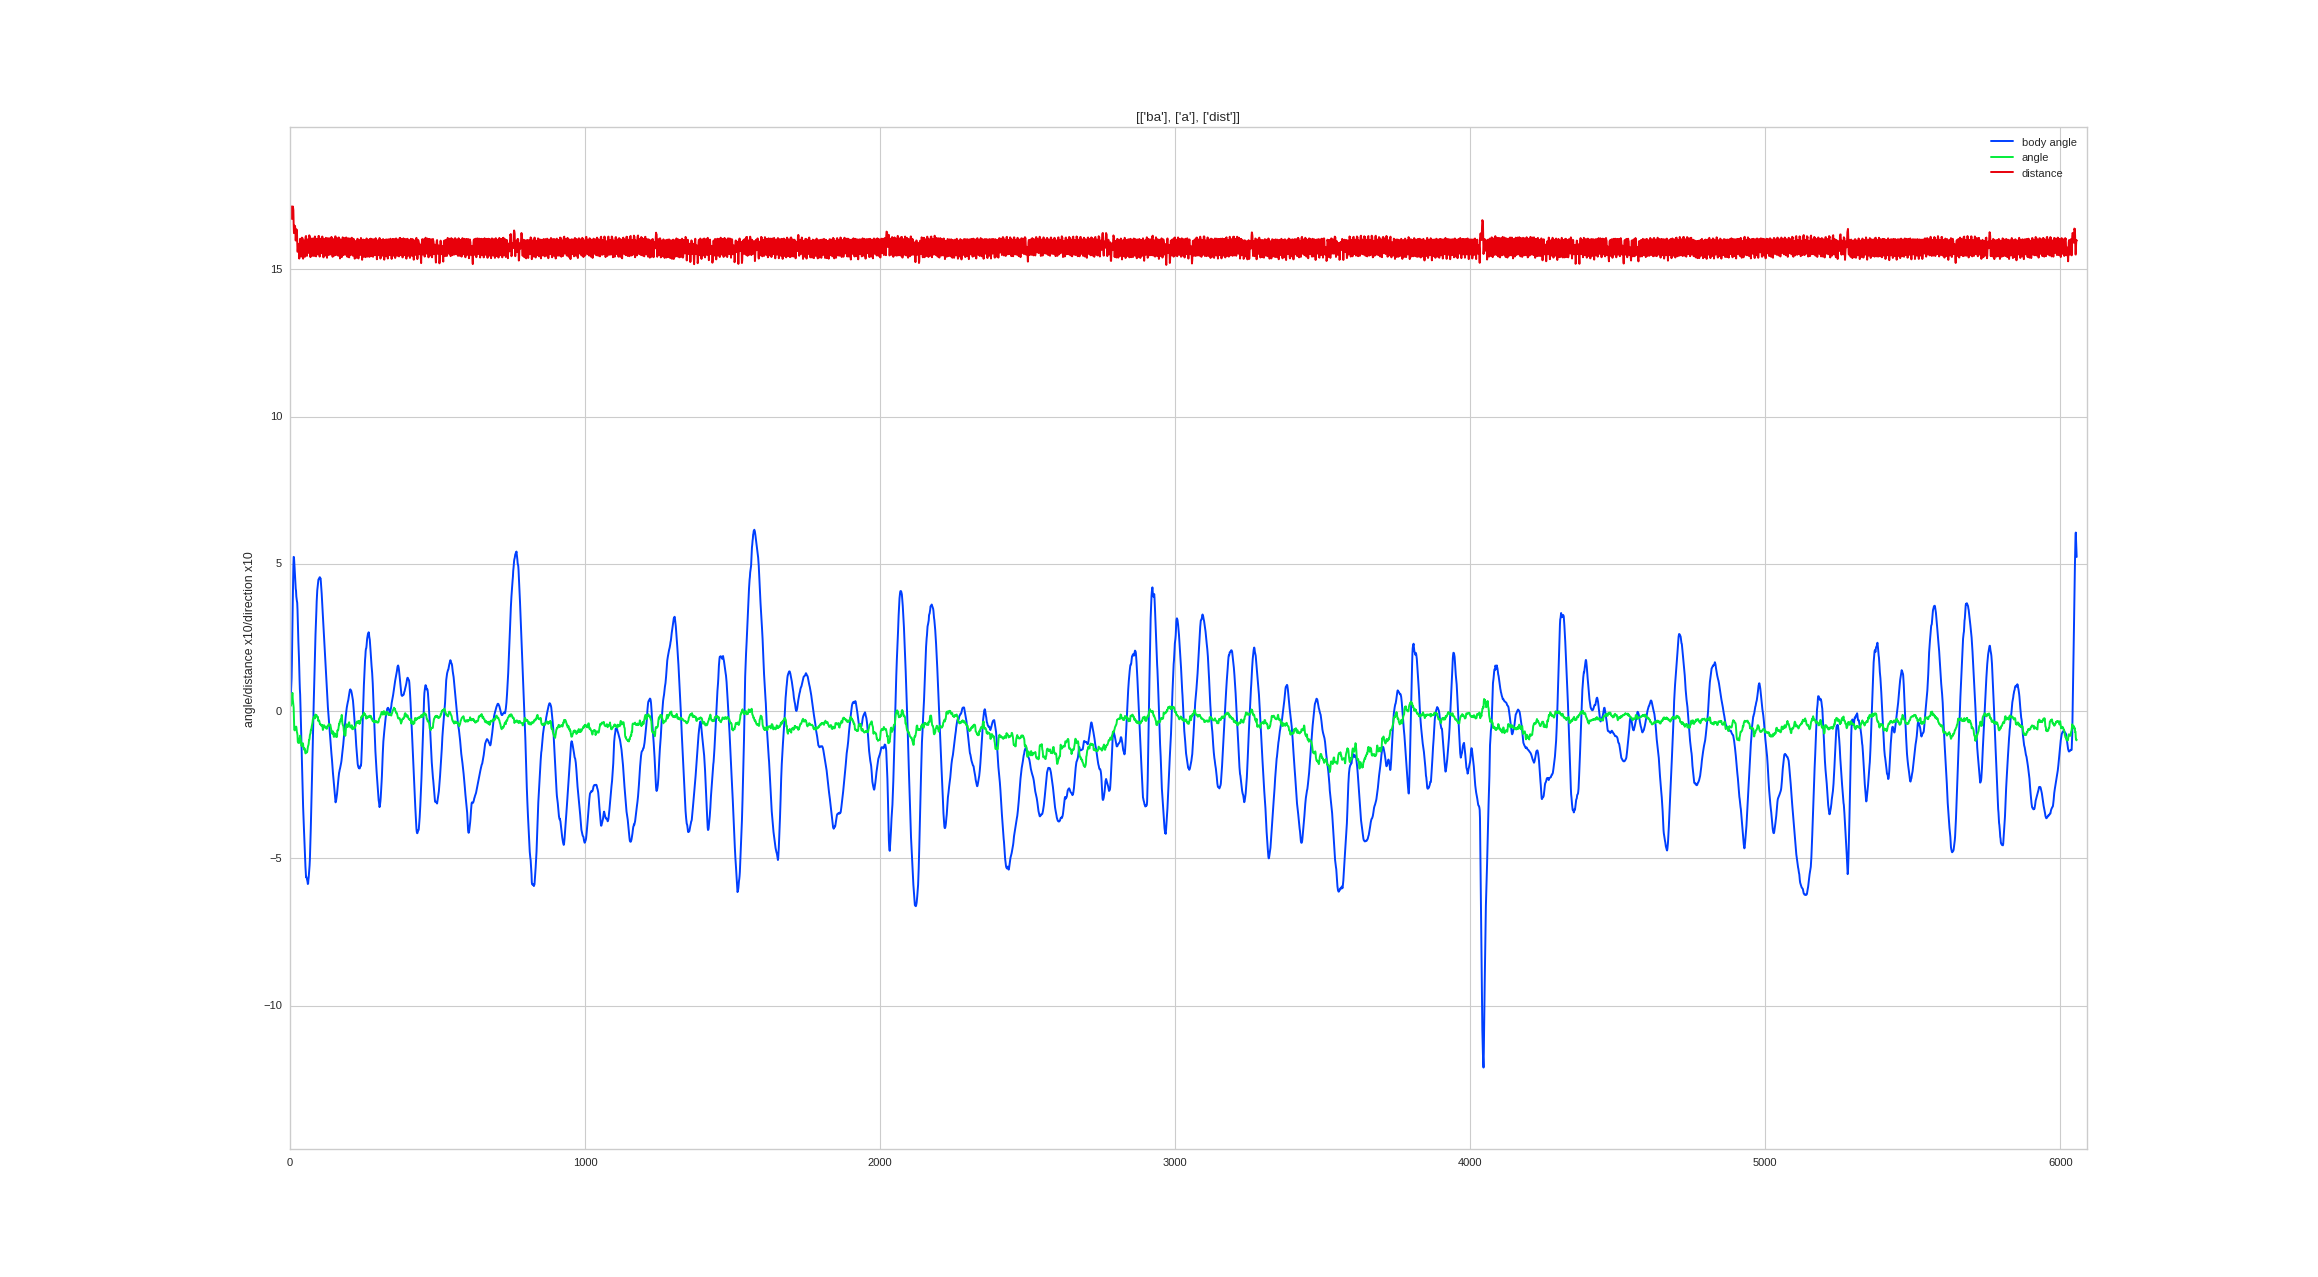
\includegraphics[width=\textwidth]{figures/plots/M2-baADist}
  \caption{ Performance of the multilayer network with the split hidden layer in the test }
  \label{fig:M2-baADist}
\end{figure}



% \begin{table}[htpb]
%   \caption[Parameters 2.Setup]{Parameters of body Neurons in the 2. setup} \label{tab:ParamsBase2N}
%   \begin{tabular}{|c| c |l|}
%       \toprule
%       Parameter & Value & Description \\
%       \midrule
%       $c_m$   & 20.0  & Capacity of the membrane \\
%       $tau_{m}$    & 50.0  & Membrane time constant \\
%       $tau_{refrac}$   & 1.  & Duration of refractory period\\
%       $v_{thresh}$   & -50.0  & Spike initiation threshold \\
%       $v_{reset}$    & -65.0  &  Reset value for $V_m$ after a spike \\
%       $v_{rest}$ & -65.0 & Resting voltage for $V_m$ \\
%       \bottomrule
%     \end{tabular}
%     \end{table}
%   \begin{table}[htpb]
%     \caption[Parameters 2.Setup]{Parameters of the body Synapses for the 2. setup} \label{tab:ParamsBase2S}
%     \begin{tabular}{|c| c |l|}
%         \toprule
%         Parameter  & Value & Description \\
%         \midrule
%         $W_{max}$ & 6000   & Maximum weight of synapse\\   
%         $W_{min}$ & -6000  & Minimum weight of synapse\\   
%         $A_{+}$   & 0.1    & Constant scaling strength of potentiation\\   
%         $A_{-}$   & -0.1   & Constant scaling strength of depression \\   
%         $\tau_c$  & 100.0   & Time constant of eligibility trace \\  
%         $\tau_n$  & 20.0   & Time constant of reward signal  \\   
%         $b$       & 0.0    & Baseline neuromodulator concentration \\    
%         \bottomrule
%     \end{tabular}
%     \end{table}


% \begin{figure}[htpb]
%   \centering
%   % This should probably go into a file in figures/
%   \begin{tikzpicture}[node distance=0.5cm]
%     \node (P0) {};
%     \node (P1) [right of=P0] {};
%     \node (P2) [right of=P1] {};
%     \node (P3) [right of=P2] {};
%     \node (P4) [right of=P3] {};
%     \node (P5) [right of=P4] {};
%     \node (P6) [right of=P5] {};
%     \node (P7) [right of=P6] {};
%     \node (P8) [right of=P7] {};
%     \node (P9) [right of=P8] {};

%     \node (I0) [below of=P0] {};
%     \node (I1) [right of=I0] {};
%     \node (I2) [right of=I1] {};
%     \node (I3) [right of=I2] {};
%     \node (I4) [right of=I3] {};
%     \node (I5) [right of=I4] {};
%     \node (I6) [right of=I5] {};
%     \node (I7) [right of=I6] {};
%     \node (I8) [right of=I7] {};
%     \node (I9) [right of=I8] {};

%     \node (O0) [below of=I0] {};
%     \node (O1) [right of=O0] {};

%     \node (D0) [below of=O0] {};
%     \node (D1) [below of=O1] {};

%     \path[every node]
%       (P0) edge (I0)
%       (P1) edge (I1)
%       (P2) edge (I2)
%       (P3) edge (I3)
%       (P4) edge (I4)
%       (P5) edge (I5)
%       (P6) edge (I6)
%       (P7) edge (I7)
%       (P8) edge (I8)
%       (P9) edge (I9)

%       (I0) edge (O0)
%       (I1) edge (O0)
%       (I2) edge (O0)
%       (I3) edge (O0)
%       (I4) edge (O0)
%       (I5) edge (O0)
%       (I6) edge (O0)
%       (I7) edge (O0)
%       (I8) edge (O0)
%       (I9) edge (O0)
      
%       (I0) edge (O1)
%       (I1) edge (O1)
%       (I2) edge (O1)
%       (I3) edge (O1)
%       (I4) edge (O1)
%       (I5) edge (O1)
%       (I6) edge (O1)
%       (I7) edge (O1)
%       (I8) edge (O1)
%       (I9) edge (O1)

%       (O0) edge (D0)
%       (O1) edge (D1);
%   \end{tikzpicture}
%   \caption[Simple Network]{Simple Network Topology}\label{fig:simpleNetwork}
% \end{figure}

\chapter{Conclusion}


% \begin{table}[htpb]
%   \caption[Parameters 2.Setup]{Parameters of body Neurons in the 2. setup} \label{tab:ParamsBase2N}
%   \begin{tabular}{|c| c |l|}
%       \toprule
%       Parameter & Value & Description \\
%       \midrule
%       $c_m$   & 20.0  & Capacity of the membrane \\
%       $tau_{m}$    & 50.0  & Membrane time constant \\
%       $tau_{refrac}$   & 1.  & Duration of refractory period\\
%       $v_{thresh}$   & -50.0  & Spike initiation threshold \\
%       $v_{reset}$    & -65.0  &  Reset value for $V_m$ after a spike \\
%       $v_{rest}$ & -65.0 & Resting voltage for $V_m$ \\
%       \bottomrule
%     \end{tabular}
%     \end{table}
%   \begin{table}[htpb]
%     \caption[Parameters 2.Setup]{Parameters of the body Synapses for the 2. setup} \label{tab:ParamsBase2S}
%     \begin{tabular}{|c| c |l|}
%         \toprule
%         Parameter  & Value & Description \\
%         \midrule
%         $W_{max}$ & 6000   & Maximum weight of synapse\\   
%         $W_{min}$ & -6000  & Minimum weight of synapse\\   
%         $A_{+}$   & 0.1    & Constant scaling strength of potentiation\\   
%         $A_{-}$   & -0.1   & Constant scaling strength of depression \\   
%         $\tau_c$  & 100.0   & Time constant of eligibility trace \\  
%         $\tau_n$  & 20.0   & Time constant of reward signal  \\   
%         $b$       & 0.0    & Baseline neuromodulator concentration \\    
%         \bottomrule
%     \end{tabular}
%     \end{table}


% \begin{figure}[htpb]
%   \centering
%   % This should probably go into a file in figures/
%   \begin{tikzpicture}[node distance=0.5cm]
%     \node (P0) {};
%     \node (P1) [right of=P0] {};
%     \node (P2) [right of=P1] {};
%     \node (P3) [right of=P2] {};
%     \node (P4) [right of=P3] {};
%     \node (P5) [right of=P4] {};
%     \node (P6) [right of=P5] {};
%     \node (P7) [right of=P6] {};
%     \node (P8) [right of=P7] {};
%     \node (P9) [right of=P8] {};

%     \node (I0) [below of=P0] {};
%     \node (I1) [right of=I0] {};
%     \node (I2) [right of=I1] {};
%     \node (I3) [right of=I2] {};
%     \node (I4) [right of=I3] {};
%     \node (I5) [right of=I4] {};
%     \node (I6) [right of=I5] {};
%     \node (I7) [right of=I6] {};
%     \node (I8) [right of=I7] {};
%     \node (I9) [right of=I8] {};

%     \node (O0) [below of=I0] {};
%     \node (O1) [right of=O0] {};

%     \node (D0) [below of=O0] {};
%     \node (D1) [below of=O1] {};

%     \path[every node]
%       (P0) edge (I0)
%       (P1) edge (I1)
%       (P2) edge (I2)
%       (P3) edge (I3)
%       (P4) edge (I4)
%       (P5) edge (I5)
%       (P6) edge (I6)
%       (P7) edge (I7)
%       (P8) edge (I8)
%       (P9) edge (I9)

%       (I0) edge (O0)
%       (I1) edge (O0)
%       (I2) edge (O0)
%       (I3) edge (O0)
%       (I4) edge (O0)
%       (I5) edge (O0)
%       (I6) edge (O0)
%       (I7) edge (O0)
%       (I8) edge (O0)
%       (I9) edge (O0)
      
%       (I0) edge (O1)
%       (I1) edge (O1)
%       (I2) edge (O1)
%       (I3) edge (O1)
%       (I4) edge (O1)
%       (I5) edge (O1)
%       (I6) edge (O1)
%       (I7) edge (O1)
%       (I8) edge (O1)
%       (I9) edge (O1)

%       (O0) edge (D0)
%       (O1) edge (D1);
%   \end{tikzpicture}
%   \caption[Simple Network]{Simple Network Topology}\label{fig:simpleNetwork}
% \end{figure}

% TODO: add more chapters here

\appendix{}

\microtypesetup{protrusion=false}
\listoffigures{}
\listoftables{}
\microtypesetup{protrusion=true}
\printbibliography{}

\end{document}
